\documentclass[10pt,a4paper,oneside]{scrreprt}
\usepackage{mystyle}

\begin{document}
\begin{titlepage}
  
\enlargethispage{10cm}

\begin{center}
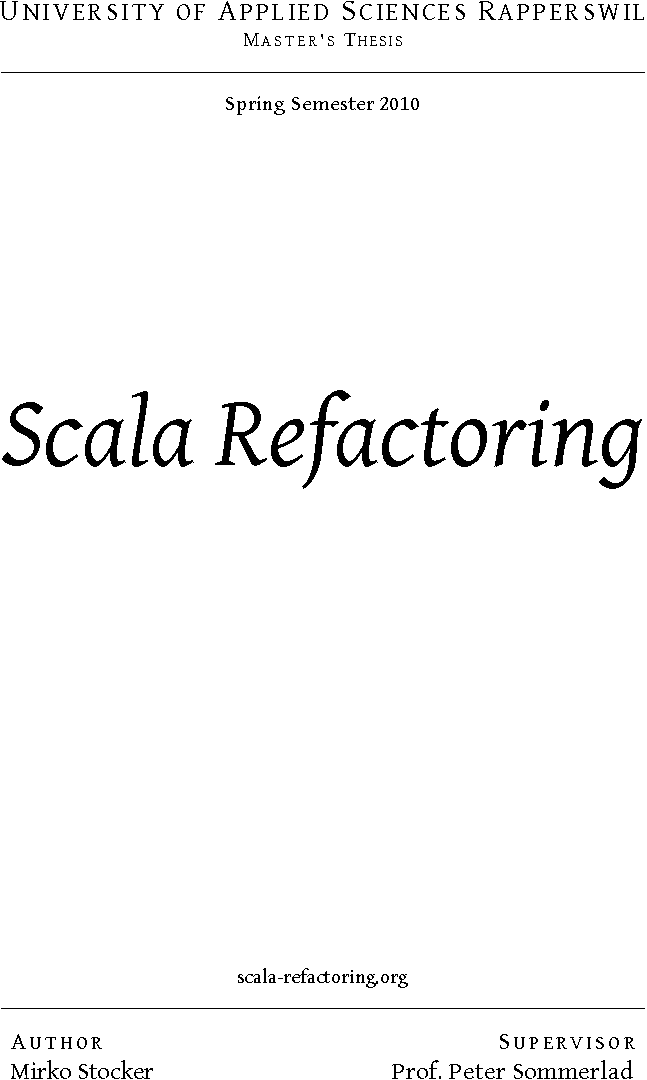
\includegraphics[width=\linewidth]{titlepage.pdf}
\end{center}

\end{titlepage}

\emptypage

\chapter*{Abstract}

\pagenumbering{roman}

Refactoring -- the technique to improve the internal structure of a program -- has become a widely adopted practice among software engineers, but manual refactoring is tedious and error prone. 

The Scala programming language is supported on all major Java development platforms, but most do not yet assist the programmer with automated refactoring tools. 

This project provides an IDE independent library to create automated refactorings for Scala. A refactoring is essentially a transformation of the abstract syntax tree. The library makes writing such transformations as simple as possible: combinators can be used to build complex transformations from basic ones. Deriving the concrete source code changes from these converted trees is handled transparently by the library.

Several refactorings have been implemented on top of the library, along with the integration into the Scala IDE for Eclipse: Rename, Extract Local, Extract Method, Inline Local and Organize Imports.

\chapter*{Management Summary}

In this thesis, we describe the development of a refactoring tool for the Scala programming language, conducted at the Institute for Software at the University of Applied Sciences Rapperswil. This master's thesis is a continuation of a previous term project by the same author.

\section*{Motivation}

Refactoring means to improve the internal structure of a program while keeping its external behavior. Improving a program's internal structure can be achieved in various ways: the names that are used internally can be changed to better reflect their functionality, or the code can be reorganized to make the program easier to extend, read, comprehend, and test. 

Refactoring does not have to be done with a specific tool, nor is it limited to a certain language or technology. Most integrated development environments support the developer with automated refactorings. Having such support reduces the time and therefore the hurdle to apply a refactoring; automation is also less error-prone than doing the same operations manually.

Scala is a modern programming language developed by Martin Odersky and his team at EPFL. Scala combines various aspects from object oriented and functional programming models. While it supports the developers with many powerful features, it is still fully compatible with code written in Java, allowing projects to mix Scala and Java.

Scala is an impressive language, but if it wants to become widely used in enterprises, it also needs to provide tools, including integrated development environments (IDEs). There already exist several Scala IDEs, but their refactoring support is still very limited.

\section*{Goals}

The primary goal of this thesis is to support Scala IDEs with automated refactoring tools. The refactoring functionality is offered in the form of a library, so it can be integrated into and shared among different IDEs and other tools that want to refactor Scala code. To demonstrate the implemented refactorings, the library has to be integrated into the Eclipse based Scala IDE. 

A second goal is to make the creation of new automated refactorings as simple as possible, to enable interested developers to implement their own refactorings. 

\section*{Results}

We have developed a library that builds on the Scala compiler and contains everything that is needed to create automated refactorings for Scala. The following refactorings have been implemented: 

\begin{description}
  \item[Rename] for all the names that are used in the source code.
  \item[Extract Method] to extract a selection of statements into a new method.
  \item[Extract Local] to introduce a new local variable for an existing expression.
  \item[Inline Local] to replace references to a local variable with its right hand side.
  \item[Organize Imports] to clean up the imported dependencies of a source file.
 \end{description}

These refactorings are all fully integrated into the Scala IDE for Eclipse, along with an online help that explains the usage of each refactoring.

To help new refactoring implementors getting started, this report documents not only the internals of the library but also the detailed implementation of the refactorings as well as how-tos and guides on how new refactorings can be written and integrated into IDEs or other tools.

The implemented refactorings are already part of the current development builds of the Scala IDE for Eclipse and have been presented at the first Scala conference -- Scala Days 2010 \cite{ScalaDaysRefactoring}.

\newpage

\chapter*{Declaration Of Authorship}

I, Mirko Stocker, declare that this thesis and the work presented in it is my own, original work. All the sources I consulted and cited are clearly attributed. I have acknowledged all main sources of help.

\vspace{3cm}

\noindent Location, Date: \hspace{1cm} \ldots\ldots\ldots\ldots\ldots\ldots\ldots\ldots\ldots\ldots\ldots\ldots\ldots\ldots\ldots\ldots\ldots\ldots \\

\vspace{1.5cm}

\noindent Signature: \hspace{1.77cm} \ldots\ldots\ldots\ldots\ldots\ldots\ldots\ldots\ldots\ldots\ldots\ldots\ldots\ldots\ldots\ldots\ldots\ldots

\newpage

\setcounter{tocdepth}{2}

\tableofcontents

\newpage

\pagenumbering{arabic}

\chapter{Introduction} \label{chapter:introduction}

The goal of this project is to provide Scala developers with automated refactoring tools. This master's thesis is a continuation of a foregoing term project (see \cite{ScalaRefactoring}) at the University of Applied Sciences Rapperswil, Switzerland. 

In this chapter, we will briefly introduce the Refactoring technique and the Scala programming language, as well as explain the goals and motivation of this thesis.

\section{Refactoring}

Refactoring of programs is a well established practice among professional software developers. In his 1992 PhD thesis \cite{OpdykeThesis}, William Opdyke defined refactoring as 

\begin{quotation}
a set of program restructuring operations (refactorings) that support the design, evolution and reuse of object-oriented application frameworks.
\end{quotation}

The breakthrough in industry started in 1999, when Martin Fowler and his colleagues published their popular book \textit{Refactoring: Improving the Design of Existing Code} \cite{FowlerRefactoring}, where refactoring is defined as 

\begin{quotation}
the process of changing a software system in such a way that it does not alter the external behavior of the code yet improves its internal structure.
\end{quotation} 

Today, refactoring has been absorbed by the programming mainstream, and is usually well integrated into the developer's work-flow and development environment. Developers use refactoring tools to keep their code maintainable by applying refactorings such as Rename to quickly change identifiers. In agile environments, where software is rapidly adapted to handle new requirements, performing refactorings regularly is essential to get reusable code and to keep up with the pace of change.

Refactoring as a technique does not mandate a tool nor depend on a specific programming language.

\section{Scala}

The Scala programming language \cite{ProgrammingScala}, developed by Martin Odersky and his team at EPFL, is a statically typed, compiled language that runs on the Java Virtual Machine (or on .NET alternatively \cite{ScalacNet}) and excels with its unique combination of object-oriented and functional programming concepts. Odersky also calls Scala a postfunctional language because it has been designed ``to make functional constructs, imperative constructs, and objects all play well together'' \cite{ScalaPostFunctional}. 

One of Scala's strengths is its seamless interoperability with Java on the class level: Scala classes can extend Java classes and vice-versa. Scala also does not ship with a huge standard library but uses existing Java classes where it is sensible.

Scala provides all of Java's object-oriented features but does away with the not really object oriented ones like primitive data types and static class members. Scala also provides code reuse via traits; a kind of interface that may contain implementations.

From functional programming, Scala has absorbed functions as first class values and embraces the idea of immutability with various language constructs. Scala even supports lazy evaluation through by-name parameters and the \src{lazy} modifier for values. A combination from both object-oriented and functional worlds can be seen in Scala's ability to use pattern matching to deconstruct objects while still preserving encapsulation.

These were just a few examples of how Scala differs from other languages such as Java. One last feature worth mentioning is that in Scala, building your own abstractions and control structures is easy, which is the reason why it has been named the ``scalable language''. For a short introduction and a tutorial, see \cite{ScalaTutorial} and \cite{ScalaByExample}.

\section{Integrated Development Environments}

Many programmers, particularly of mainstream languages such as Java and C\#, use integrated development environments (IDE) to create their software. Notably the IDEs for the Java programming language excel with automated refactoring support; the screen-shots in \figref{figure:ide_refactorings} show two examples. If Scala wants to cater to those programmers and become a viable alternative in enterprises, it needs to offer IDE support that is as comfortable to use and as mature as the existing Java tooling is.

Scala is supported on the three main Java development platforms Eclipse \cite{EclipseScalaIDE}, IntelliJ IDEA \cite{IntelliJScalaIDE}, and NetBeans \cite{NetBeansJScalaIDE}, but with the exception of IntelliJ IDEA -- which offers a few refactorings -- support for automated refactoring does not yet exist. Although a study by Emerson~Murphy-Hill et al. among developers using Eclipse \cite{RefactoringStudy} indicates that many refactorings are not performed with the tool support but by hand, other automated refactorings like Rename, Move and Extract Method are used frequently.

\begin{figure}
 \centering
 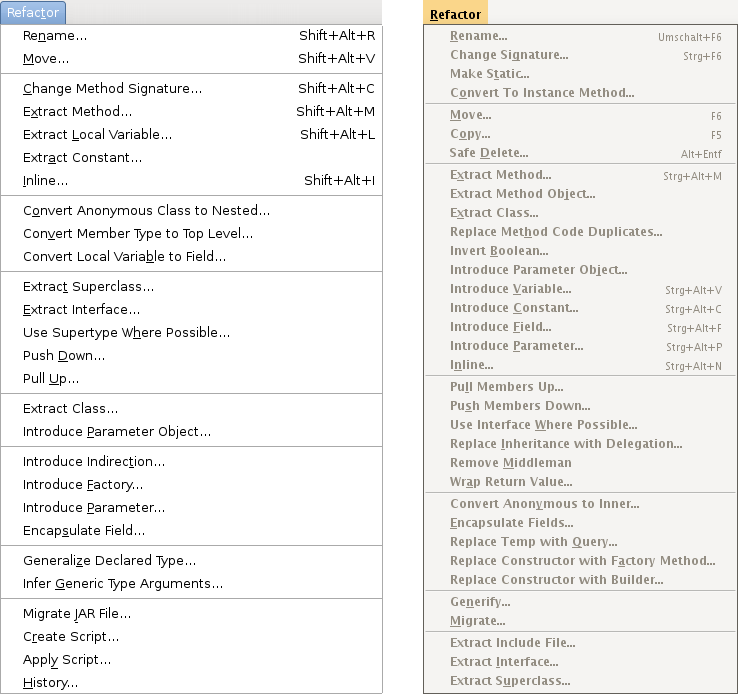
\includegraphics[width=0.7\linewidth]{ide_refactorings.png}
 \caption{Automated refactoring in Java IDEs}
 \label{figure:ide_refactorings}
\end{figure}

\section{Thesis Goals}

The goal of this thesis is to support Scala IDEs with automated refactoring tools. It aims to provide a comprehensive catalog of refactorings and the necessary infrastructure to create new refactorings. To maximize the number of IDEs and other tools that can profit from the project, it will provide an IDE independent refactoring library that only depends on the Scala compiler. IDEs can then seamlessly integrate this library by providing the user interface and interaction.

As most IDEs today are written in Java, integrating a Scala library is no problem. Also, because the majority of Scala IDEs are completely open source (NetBeans, Eclipse), having a single refactoring library allows their developers to cooperate on an implementation, not fragmenting the already scarce resources any further. As a showcase, this project provides the integration into the Eclipse based Scala IDE \cite{EclipseScalaIDE}.

Writing an automated refactoring is no trivial task, several things have to be taken care of: one has to analyze the source code, create an appropriate representation (e.g. abstract or concrete syntax tree) of the program, transform it and turn it back into plain source code. 

The heart of a refactoring is the transformation or manipulation of the program representation; but often -- from our experience with refactoring tools for languages like Ruby \cite{RubyRefactoring}, C++ \cite{CdtOopsla}, and Groovy \cite{GroovyOopsla} -- the developer also has to provide the instructions how these manipulations affect the source code, or how the changes made to the AST are to be translated back into source code changes. This makes creating new refactorings unjustifiably more complex and is a high entry barrier for contributors. The Scala refactoring library tries to make creating new refactorings as simple as possible: code generation from the abstract syntax tree is completely transparent and needs almost no guidance from the refactoring writer.

Transformations of the program are based on the Scala compiler's own AST, and are written in a functional programming style that makes it possible to assemble complex transformations from simple ones using combinators.

To summarize, the Scala Refactoring project develops an IDE independent refactoring library that makes creating new refactorings as simple as possible.

\section{Contents of This Report}

This document is organized as follows: Chapter~\vref{chapter:refactoring-library} explains the concepts and implementation of the refactoring library. The details of the implemented refactorings are described in Chapter~\vref{chapter:implemented-refactorings}. How these refactorings can be integrated into an IDE or other tool is the topic of Chapter~\vref{chapter:tool-integration}. How the implemented refactorings are tested is explained in Chapter~\vref{chapter:testing}. Chapter~\vref{chapter:outlook} concludes this thesis with a review of the achievements and an outlook on further work.

The project environment is briefly explained in Appendix~\vref{chapter:project-environment}. The appendices also contain a user guide to the refactorings in Eclipse (Appendix~\vref{chapter:user-guide}), and a how-to introduction for developers that explains how a new refactoring can be created in Appendix~\vref{chapter:developer-how-to}. Developers that work with Scala's AST might also be interested in Appendix~\vref{chapter:scala-ast}, where the specific trees of the AST are described. Appendix~\vref{chapter:advanced-scala-features} contains explanations of more advanced Scala features and is referenced where needed in this document. The source code of this thesis is released under the Scala license, which is printed in Appendix~ \vref{chapter:scala-license}

\section{Target Audience}

We assume that the reader knows the basic Scala concepts (if not, Scala by Example \cite{ScalaByExample} is a good starting point) and is able to read Scala source code. Whenever more advanced or possibly confusing concepts are used, a reference to Appendix~\ref{chapter:advanced-scala-features} will be provided.

Developers who want to use the library to transform Scala source code should read Chapter~\vref{chapter:refactoring-library} on the library internals and Appendix~\vref{chapter:scala-ast} to learn more about Scala's AST. 

To integrate the existing refactorings in a new tool, Chapter~\vref{chapter:tool-integration} shows how this can be done with a made up editor and how the integration into the Scala IDE for Eclipse looks like.

For those wishing to implement new refactorings, the how-to in Appendix~\vref{chapter:developer-how-to} and Chapter~\vref{chapter:implemented-refactorings} on the implemented refactorings can serve as a starting point. How the new refactoring can be tested is explained in Chapter~\vref{chapter:testing}.

Users who wish to provide accurate bug reports should take a look at Chapter~\vref{chapter:testing} on testing to learn how a new test that points out a failure can be implemented.

\chapter{Refactoring Library} \label{chapter:refactoring-library}

\chapter{Refactoring Library} \label{chapter:refactoring-library}

The refactoring library is the heart of the Scala Refactoring project. It contains the means to analyze a Scala program, to transform it and to turn it back into source code. When writing a refactoring, one usually has to implement the following steps:

\begin{itemize}
 \item provide a user interface so that a specific refactoring can be discovered and invoked from the IDE.
 \item analyze the program under refactoring to find out whether the refactoring is applicable and further to determine the parameters and constraints for the refactoring.
 \item transform the program tree from its original form into a new -- refactored -- form according to the refactoring's configuration.
 \item turn this new form back into source code, keeping as much of the original formatting in place as possible and to generate code for new parts of the program.
 \item present the result of the refactoring to the user -- typically in the form of a patch --  and apply it to the source code.
\end{itemize}

From all these steps, the first and the last one are IDE-platform dependent and usually well supported (see Chapter XXX). For the other three, the refactoring library contains the necessary infrastructure to make these steps as simple as possible.

The essence of a refactoring is a transformation that takes a program in some abstract form and changes its structure. To know what to transform, one has to analyze the program first. That we also have to turn a refactored program back into source code is a consequence of storing programs as plain text files, but is not an essential part of a refactoring. Therefore, one of the design goals was to provide a generic implementation that can handle all kinds of changes without any help from the transformation phase.

In the remainder of this chapter, we shall first take a look at the architecture of the library and then describe each of the three main components in detail.

\section{Overview}

% Muss ich den AST erkl�ren? Warum es den braucht und so?

Refactorings typically do not work on the source code directly but -- just as the Scala compiler -- do most of the work on the abstract syntax tree (AST) of the program. We also do not create our own AST but reuse the Scala compiler's (as explained in Chapter XXX, we also do not invoke the compiler ourselves but just take an AST from the IDE). This not only saves time but also makes it easier to implement a new refactoring if one is already familiar with the Scala compiler's AST.

The Scala's AST is explained in more detail in Appendix \vref{chapter:scala-ast}. A general knowledge on what an AST is should suffice to follow the explanations in this chapter. Useful to know is that all trees have a position information: either indicating a location from where the tree origins or a \src{NoPosition}, which denotes trees that do not have a corresponding source code location. This information is later used by the transformation and code generation.%: trees with a \src{NoPosition} are pretty printed and the trees with a specific source location are reused (this is needed to preserve the formatting of the source code).

A typical refactoring first takes the current file's AST and the user's selection or caret position and first checks if the chosen refactoring is applicable. The AST is then transformed into its new form and handed over to the source generator to turn the AST back into source code (see \figref{figure:refactoring-flow} for a visualization of this workflow). As motivated above, generating the source code is already implemented generically and needs no further instructions from the refactoring implementor.

\begin{figure}
  \centering
  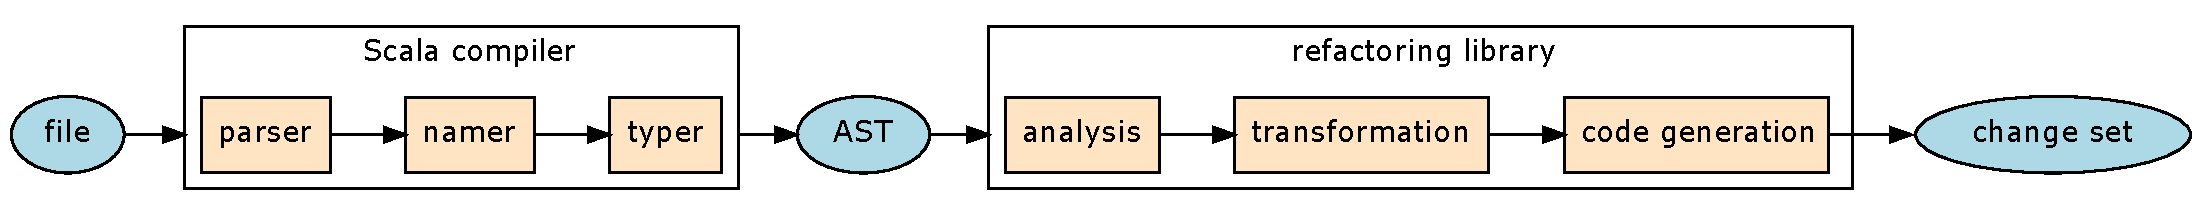
\includegraphics[width=\linewidth]{refactoring-flow.pdf}
  \caption{The work-flow of the refactoring. The IDE uses the compiler to parse the source file and passes the resulting syntax tree to the refactoring tool. The result of a refactoring is a set of changes, viz. a patch, that the IDE has to apply to the source files (adapted from \cite{ScalaRefactoring}).}
  \label{figure:refactoring-flow}
\end{figure}

The architecture (see \figref{figure:refactoring-architecture}) and also the source code layout follow these three steps:

\begin{description}
 \item[Analysis] in package \src{analysis} contains the means to analyze the program and to build an index for the identifiers in the program. This will be explained further in Section \vref{section:analysis}.
 \item[Transformation] in package \src{transformation} provides a framework to write, combine and apply transformations on trees, as well as some factory methods to create new trees. How these work is described in Section \vref{section:transformation}.
 \item[Source Generation] in package \src{sourcegen} mainly contains the \src{SourceGenerator} that turns an AST back into change objects (i.e. patches) for the source code as explained in Section \vref{section:source-generation}.
\end{description}

\begin{figure}
  \centering
  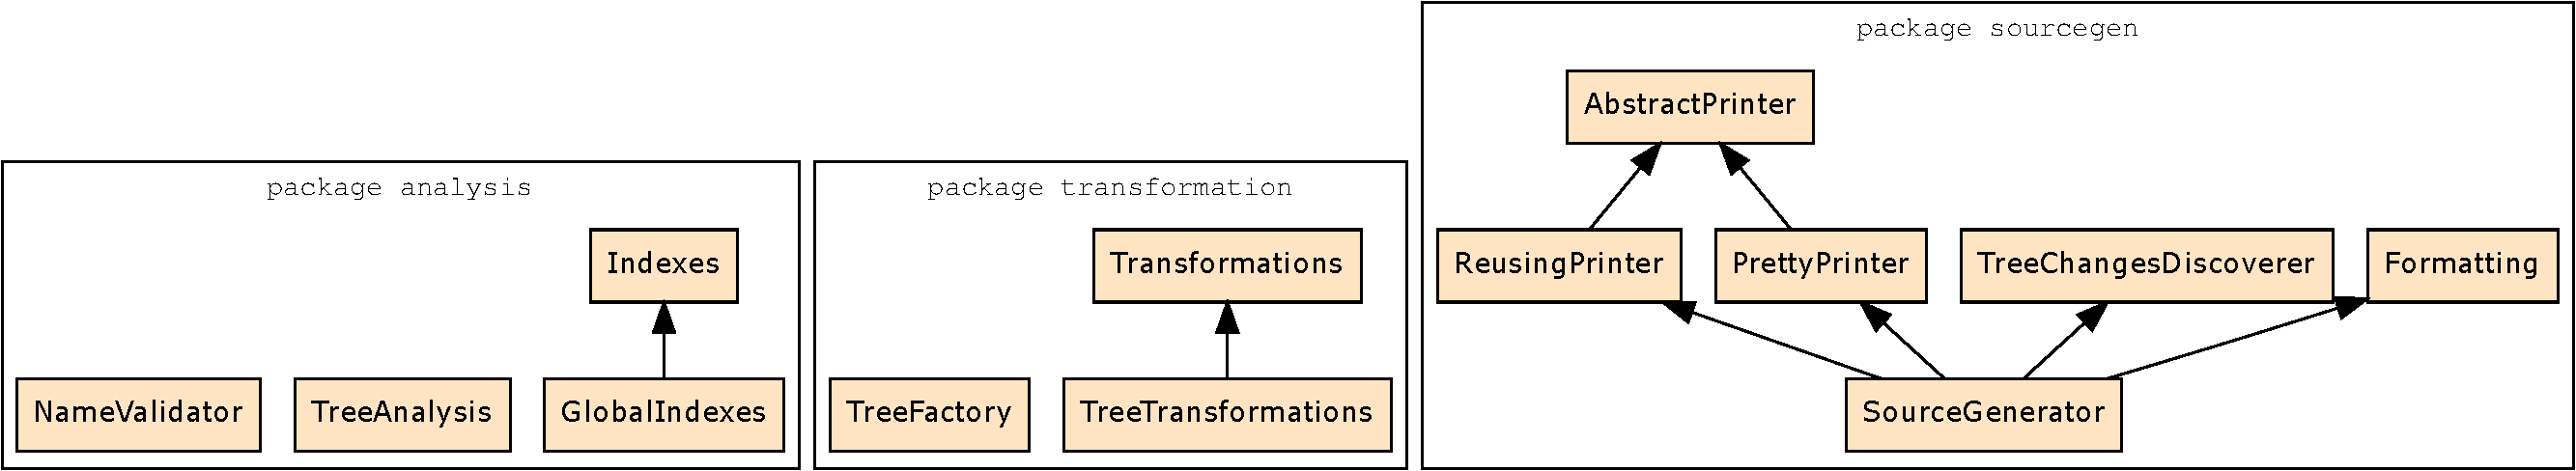
\includegraphics[width=\linewidth]{refactoring-architecture.pdf}
  \caption{An overview of the refactoring library architecture: the three main packages \src{analysis}, \src{transformation}, and \src{sourcegen}. Note that there exist more traits and classes in these packages -- but for the sake of clarity, only the major ones are shown.}
  \label{figure:refactoring-architecture}
\end{figure}

% path dependent type, global?

In the remainder of this chapter, the three library components will be explained in more detail. Keep in mind that the shown functionality is not meant to be feature complete but can and will be extended as seen fit. %geh�rt das hier hin?

\section{Analysis} \label{section:analysis}

An import step in each refactoring is to analyze the current program that is being refactored. For example, when doing a Rename refactoring, we need to resolve all references to the renamed name. A more complex example is Extract Method, where we need to perform data-flow analysis to determine the parameters and return values of the extracted method.

Our IDEs also analyze the program code in a similar way to make the life of the programmer easier: finding the declaration of a variable or listing all subtypes of a class are common operations.

Our analyses heavily depend on the Scala compiler's AST and all the information it provides through the program's symbols. For example, each symbol has an owner that can be used to navigate the logical structure of the program. There are also almost one hundred \src{isXY} methods defined on the \src{Symbol} class that can be used to query information:

\begin{lstlisting}
abstract class Symbol {
  %\ldots%
  def isAnonymousClass: Boolean
  def isConstructor: Boolean
  def isGetter: Boolean
  def isLocal: Boolean
  def isSubClass(that: Symbol): Boolean
  %\ldots%
}
\end{lstlisting}

All the trees that inherit from the \src{SymTree} trait provide a symbol instance, where \src{DefTrees} usually introduce a new symbol and \src{RefTrees} reference a symbol from a \src{DefTree}. The following illustration shows how symbols are related (not all symbols are colored, for example, the built in types have a symbol as well):

\begin{lstlisting}
trait %\bluebox{SuperClass}% {
  def %\greenbox{strlen}%(%\redbox{str}%: String) = %\redbox{str}%.length
  def %\lgreenbox{abstractMethod}%: Int
}

class %\yellowbox{SubClass}% extends %\bluebox{SuperClass}% {
  def %\greybox{abstractMethod}% = 1 + %\greenbox{strlen}%("1")
}
\end{lstlisting}

Note that the two \src{abstractMethod} symbols are not the same, but there are other means to find overriden and implemented methods in subclasses, as we shall see later.

While the trees can have a reference to a symbol, the converse is not true: symbols do not know about the trees they are related to. But for refactoring, this information is crucial. This is why the refactoring library contains the means to build an index that relates symbols and corresponding trees.

\subsection{Refactoring Index Interface}

Building an index over a whole project can be expensive, so ideally, the IDE would maintain the index and pass it to the refactoring library when need, in the same way that the library does not compile the source files itself but gets the ASTs directly from the IDE.

The interface that needs to be implemented and is used by the refactorings to query the index looks as follows (note that \src{global} is an instance of the compiler that is provided by an outer trait so the trees can be used as path dependent types (see Appendix \vref{section:path-dependent-types})):

\begin{lstlisting}
trait IndexLookup {
  /**
    * Returns all defined symbols, i.e. symbols of DefTrees.
    * */
  def allDefinedSymbols(): List[global.Symbol]
  
  /**
    * Returns all symbols that are part of the index, either referenced or defined.
    * */
  def allSymbols(): List[global.Symbol]    
  
  /**
    * For a given Symbol, tries to find the tree that declares it.
    * */
  def declaration(s: global.Symbol): Option[global.DefTree]
  /**
    * For a given Symbol, returns all trees that contain a reference to it.
    * */
  def references(s: global.Symbol): List[global.Tree]
  
  /**
    * For a given Symbol, returns all trees that reference or declare the Symbol.
    * */
  def occurences(s: global.Symbol): List[global.Tree]

  /**
    * For the given Symbol - which can be a class or object - returns a list of all sub- 
    * and super classes, in no particular order.
    */
  def completeClassHierarchy(s: global.Symbol): List[global.Symbol] =
    (s :: (allDefinedSymbols filter (_.ancestors contains s) flatMap (s => s :: s.ancestors)) 
      filter (_.pos != global.NoPosition) distinct)

}
\end{lstlisting}

The library also contains a default implementation that can be used if the IDE does not already maintain an index itself, as described in the following section.

\subsection{Default Index Implementation}

Building an index can be expensive: whenever a compilation unit in the program changes, references to the symbols from other compilation units can change, and also the other way around. Because of this, it is expensive to maintain one monolithic index that needs to be recreated on every change in the program. The provided implementation avoids this by maintaining a data structure for each compilation unit and combining these for queries. The implementation comprises these parts:

\begin{description}
 \item[CompilationUnitIndex] One index per compilation unit that holds the references and declarations of just this part of the program.. This structure can be rebuilt everytime a compilation unit changes. Rebuilding it traverses the whole tree once and stores mappings from symbols to \src{RefTrees} and \src{DefTrees}.
 \item[GlobalIndex] An implementation of the \src{IndexLokup} trait that ties together any number of these per compilation unit indices, but is completely stateless itself.
\end{description}

Whenever a compilation unit changes, just a single \src{CompilationUnitIndex} needs to be rebuilt and combined with the already existing ones into a new \src{GlobalIndex}.

\subsection{Resolving References}

Resolving the declaration tree of a symbol is an inexpensive lookup, but the reverse -- finding all references -- causes more work. In \src{GlobalIndex}, the process of finding all references is done in multiple steps: first, the symbol is \textit{expanded} and second all references to these expanded symbols are collected. What do we mean by expanding a symbol? Consider the example of the colored symbols we mentioned at the beginning of Section \ref{section:analysis}. The implementing method defines a different symbol than the abstract declared method. But when we want to find references, we need all references to both symbols. The same is true for getters and setters: renaming a class parameter also needs to rename all usages of getters and setters. To do this, the index implementation uses so called \src{SymbolExpanders}:

\begin{lstlisting}
trait SymbolExpander {
  def expand(s: Symbol): List[Symbol] = List(s)
}
\end{lstlisting}

The \src{SymbolExpander} is used as a stackable trait (see Appendix \vref{section:stackable-traits}) and is at the time of this writing implemented in the following variations:

\begin{description}
 \item[ExpandGetterSetters] connects getters, setters and the underlying field as well as constructor parameters. This can be done with the symbol alone and 
 \item[SuperConstructorParameters] resolves class parameters that are passed to a superconstructor.
 \item[Companion] to find the companion objects or class for a symbol.
 \item[OverridesInClassHierarchy] searches for a symbol in all sub- and superclasses. that might override or implement it.
\end{description}

The \src{GlobalIndex} uses all these traits, but it would also be possible for an implementation of the index to use only a subset of these to improve the performance. So when for example all references to a method need to be found, the initial symbol is run through all the expanders until a fix point is reached.

The following graphic illustrates the process with an example; circles represent symbols and squares trees. We start with a single symbol on the left -- e.g. a class field -- and in the first step, it is expanded to two symbols -- for example because the class field has a getter method. We do another round of expansion and find yet another related symbol (the getter might be overridden in a subclass). The third expansion yields no new symbols, thus the fourth step concludes by collecting all references and declarations to these symbols.

\begin{center}
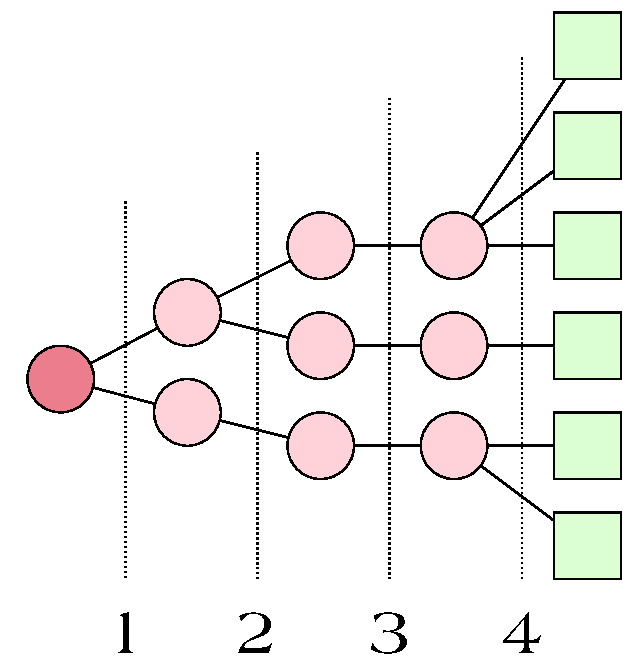
\includegraphics[width=0.5\linewidth]{expanding_symbols.pdf}
\end{center}

\subsection{Tree Analysis}

Besides the index to lookup references and declarations, some refactorings need more sophisticated analysis of the program. This section introduces the \src{TreeAnalysis} trait which contains these functionality.

\subsubsection{Local Dependencies}

The Extract Method refactoring extracts a selection of expressions into a new method. To do this, it needs to calculate all dependencies the selected expressions have to their enclosing scopes. Variables and functions that are not accessible from the new method location need to be passed as arguments, and program elements that are declared inside the extracted method and used outside of the selection need to be passed back.

In the following listing, the user wants to extract the selected expressions:

\begin{lstlisting}
def calculate {
  val sumList: Seq[Int] => Int = _ reduceLeft (_+_)
  val prodList: Seq[Int] => Int = _ reduceLeft (_*_)
  val values = 1 to 10 toList
  %\bluebox{val     sum = sumList(values)}%
  %\bluebox{val product = prodList(values)}%

  println("The sum from 1 to 10 is "+ sum +".")
}
\end{lstlisting}

The refactoring has to create a method that takes the \src{values} and the \src{sumList} and \src{prodList} functions as arguments. Also, because the \src{sum} value is used in the originating method -- but not \src{product} -- it has to be returned from the new method.

The calculation of these inbound and outbound dependencies is done as follows:

\paragraph{Inbound:} Find all symbols that are declared in the current scope (e.g. the method we extract from) and remove all declarations that are defined inside the selection. This gives us all the inbound parameters.

\paragraph{Outbound:} For each symbol that is definde inside the selection, check if it is used anywhere outside the selection.

\subsection{Name Validation}

When doing refactoring, one often has to introduce new names into the program, that can potentially conflict with an already existing name that is currently in scope. The \src{NameValidation} trait offers the functionality to check whether a name is a valid identifier -- based on the Scala compiler -- and checking if a name will collide with an already existing name:

\begin{lstlisting}

\end{lstlisting}



\section{Transformation} \label{section:transformation}

At the heart of every refactoring lies a \textit{transformation} that takes the current program in its abstract syntax tree form and transforms it into its refactored form. Such a transformation can be as simple as changing names -- think of the Rename refactoring -- or restructure large parts of the AST as in an Extract or Move refactoring. 

Often, a larger refactoring comprises many smaller transformations. An illustrative example is the Extract Method refactoring, which can be assembled from three basic transformations:

\begin{description}
 \item[Create Method] to introduce a new (empty) method.
 \item[Copy Statements] to copy the selected statements into the newly created method.
 \item[Replace Statements] to replace the original statements that have been copied to the new method with a call to it.
\end{description}

The \textit{replace} transformation itself is again a combination of two even more fundamental transformations: \textit{insert} and \textit{delete}. Once we have our Extract Method transformation, it can then again be combined with other transformations -- for example into an Extract Class refactoring. It should be clear from this that the key to a reusable refactoring library lies in the composability of its transformations. 

Conceptually, chaining simple transformations to build more powerful ones follows the Unix pipes philosophy. The design of this implementation was inspired by the Stratego program transformation tool-set (referenz) and the Kiama language processing library (referenz). Functional programming also uses the term \textit{combinator} to denote functions that can be combined and yield new functions of the same kind. An example of this are parser combinators (referenz), which are part of the Scala standard library.

In contrast to unix pipes that operate on their input line by line, performing transformations on a tree datastructure adds an additional dimension. When transforming trees, we are also concerned with questions on how we want to traverse the tree -- i.e. pre-order or post-order -- and to which children a transformation should be applied. The presented implementation handles all these concerns in a uniform way.

In the remainder of this section, we will develop the basics of the Scala refactoring's transformation combinators and show examples of their usage.

\subsection{Transformations}

A refactoring transformation is essentially a function that transforms a tree into an other tree. But because most transformations do not apply to all kinds of possible trees, we model a transformation as a function of type $Tree\Rightarrow Option[Tree]$, making use of Scala's \src{Option} monad to indicate the potential inability to transform. In the actual implementation, the transformations are implemented generically as a \src{Transformation[A,~B]} that extend \src{A~$\Rightarrow$~Option[B]}:

\begin{lstlisting}
abstract class Transformation[A, B] extends (A %$\Rightarrow$% Option[B]) {
  self %$\Rightarrow$%

  def apply(in: A): Option[B]
%\ldots%
}
\end{lstlisting}

The explicit self type annotation (see Appendix \vref{section:self-type-annotation}) will be used later in the implementation of the combinators. Note that all transformations are implemented polymorphic, but to make the explanations more clear, we will assume that they are used to transform trees.

Transformations can be created from partial functions using the \src{transformation} convenience function. As an example, we create a transformation that reverses the order of a class, trait, or object's member definitions and apply it to a given template instance.

\begin{lstlisting}
def transformation[A, B](f: PartialFunction[A, B]) = new Transformation[A, B] {
  def apply(t: A): Option[B] = f lift t
}

val reverseTemplateMembers = transformation[Tree, Tree] {
  case t: Template %$\Rightarrow$% t copy (body = t.body.reverse)
}

val result: Option[Tree] = reverseTemplateMembers(template)
\end{lstlisting}

Now that we have a way to create single transformations, we need to be able to combine them. To do this in various ways, we introduce several combinators. We use a notational shortcut to denote transformations: $A \overset{t}{_\rightarrow} [B]$ is a \src{Transformation [A, B]}.

There also exist two basic transformations, one that always succeeds, returning its input unchanged, and one that always fails, independent of its input. Depending on the context, the alias \src{id} for \src{succeed} might be a better fit and is provided as well.

\begin{lstlisting}
def succeed[A] = new Transformation[A, A] {
  def apply(a: A): Option[A] = Some(a)
}

def id[A] = success[A]

def fail[A] = new Transformation[A, A] {
  def apply(a: A): Option[A] = None
}
\end{lstlisting}

\subsection{Combinators}

There are several existing combinators already implemented in the library. On the right side of each paragraph, the symbolic or alphanumeric name and type of the transformation is shown.

\paragraph{Sequence} \hfill \lstinline{&>: } $(A \overset{t}{\rightarrow} [B]) \Rightarrow (B \overset{t}{\rightarrow} [C]) \Rightarrow (A \overset{t}{\rightarrow} [C])$

\vspace{7pt} Combines two transformations so that the second one is only applied when the first one succeeded. The result of the first transformation is passed into the second one. This is implemented as the \src{andThen} method -- or alternatively with the \src{\&>} operator -- on \src{Transformation}, which takes the second transformation as a by-name parameter:

\begin{lstlisting}
abstract class Transformation[A, B] extends (A %$\Rightarrow$% Option[B]) {
  self %$\Rightarrow$%

  def apply(in: A): Option[B]

  def andThen[C](t: %$\Rightarrow$% Transformation[B, C]) = new Transformation[A, C] {
    def apply(a: A): Option[C] = {
      self(a) flatMap t
    }
  }
  def &>[C](t: %$\Rightarrow$% Transformation[B, C]) = andThen(t)
%\ldots%
\end{lstlisting}


\paragraph{Alternative} \hfill \lstinline{|>: } $(A \overset{t}{\rightarrow} [B]) \Rightarrow (A \overset{t}{\rightarrow} [B]) \Rightarrow (A \overset{t}{\rightarrow} [B])$

\vspace{7pt} Combines two transformations so that the second one is only applied in case the first one fails. The implementation is directly based on the underlying \src{Option} type in the \src{orElse} method on \src{Transformation} and also has an operator alias:

\begin{lstlisting}
abstract class Transformation[A, B] extends (A %$\Rightarrow$% Option[B]) {
  self %$\Rightarrow$%

  def apply(in: A): Option[B]

  def orElse(t: %$\Rightarrow$% Transformation[A, B]) = new Transformation[A, B] {
    def apply(a: A): Option[B] = {
      self(a) orElse t(a)
    }
  }
  def |>(t: %$\Rightarrow$% Transformation[A, B]) = orElse(t)
%\ldots%
\end{lstlisting}

With these two combinators, we are already able to represent conditional transformations. For example, given a transformation \src{isClass} that acts as a predicate, and two transformations \src{a} and \src{b} that represent the two possible branches the transformation can take, we can combine them into a new transformation \src{isClass \&> a |> b} that executes the \src{a} transformation if the \src{isClass} transformation succeeds or \src{b} if either \src{isClass} or \src{a} fails.

Note that due to Scala's precedence rules, the \src{|>} combinator has a lower precedence than \src{\&>}.

\paragraph{Predicate} \hfill \lstinline{predicate: } $(A \overset{?}{\rightarrow} Boolean) \Rightarrow (A \overset{t}{\rightarrow} [A])$

\vspace{7pt} As we have seen, transformations can be used as predicates. We often want to construct a predicate from a function that returns a boolean value. This can be done with the \src{predicate} function which create a transformation from a partial function.

\begin{lstlisting}
def predicate[A](f: %$\Rightarrow$% PartialFunction[A, Boolean]) = new Transformation[A, A] {
  def apply(a: A): Option[A] = if (f.isDefinedAt(a) && f(a)) Some(a) else None
}
\end{lstlisting}

\paragraph{Not} \hfill \lstinline{!: } $(A \overset{t}{\rightarrow} [A]) \Rightarrow (A \overset{t}{\rightarrow} [A])$

\vspace{7pt} A combinator that inverts a transformation. Given a transformation that succeeds, then \src{not} will fail. Should the given transformation fail, then \src{not} returns the original input unchanged. This behavior is useful for transformations that act as predicates; \src{not} can be implemented using the \src{fail} and \src{id} transformations as follows.

\begin{lstlisting}
def not[A](t: %$\Rightarrow$% Transformation[A, A]) = t &> fail |> succeed
\end{lstlisting}

Now that we have several means to specify and combine our transformations, we also need a way to apply them to a whole AST, instead of just single tree nodes. For this, there exist several traversal strategies.

\subsection{Traversal}

Applying a transformation to a single tree element is not difficult, but once we want to traverse the whole AST, we need a way to apply a transformation to all children of a tree node and to construct a new tree from the result of the transformation operation. Note that traversal strategies are also just transformations that can again be combined.

\paragraph{All Children} \hfill  $allChildren: (A \overset{t}{\rightarrow} [B]) \Rightarrow (A \overset{t}{\rightarrow} [B])$

\vspace{7pt} Takes a transformation and creates a new one that applies the given transformation to all children, returning a single tree. Because there is no generic way to get all children and construct a new tree, we constrain the type parameter \src{A} to be convertible to $(A \Rightarrow B) \Rightarrow B$. This means that the user of the generic transformation has to pass us its children and create a new tree. When a child cannot be transformed, \src{allChildren} immediately aborts and returns \src{None}.

\begin{lstlisting}
def allChildren[A <%\%% (A %$\Rightarrow$% B) %$\Rightarrow$% B, B](t: %$\Rightarrow$% Transformation[A, B]) = new Transformation[A, B] {
  def apply(a: A): Option[B] = {
    Some(a(child %$\Rightarrow$% t(child) getOrElse (return None)))
  }
}
\end{lstlisting}

\src{X <\% Y} is called a \textit{view bound} and demands that there exists an implicit conversion from type \src{X} to \src{Y} (see Appendix \vref{section:implicit-conversions}). This is less constrictive than \src{X <: Y}, where \src{X} has to be a subtype of \src{Y}. In our case, we can then treat \src{a} as if it were of type \src{(A $\Rightarrow$ B) $\Rightarrow$ B}. This allows us to apply the transformation to the children of \src{a}.

\paragraph{Matching Children} \hfill $matchingChildren: (A \overset{t}{\rightarrow} [A]) \Rightarrow (A \overset{t}{\rightarrow} [A])$

\vspace{7pt} The \src{allChildren} traversal only succeeds when the transformation can be applied to all children. If children that cannot be transformed should simply be kept and passed to the new tree unchanged, we can use the \src{matchingChildren} transformation.

\begin{lstlisting}
def matchingChildren[A <%\%% (A %$\Rightarrow$% A) %$\Rightarrow$% A](t: Transformation[A, A]) = allChildren(t |> id[A])
\end{lstlisting}

Using the \src{id} transformation, we retain the original tree should the transformation not be applicable. A consequence of this is that the transformation needs to be done between the same types.

%\paragraph{Once} \hfill \lstinline{once: } $(A \overset{t}{\rightarrow} [A]) \Rightarrow (A \overset{t}{\rightarrow} [A])$

%\vspace{7pt} Applies a transformation and stops on the first successful application... not yet implemented.

The next step after being able to apply a transformation to a tree or all of its children is to expand this to the AST as a whole. We can distinguish between two fundamental ways of transforming a tree: either in a pre-order or post-order fashion.

\paragraph{Pre-Order} \hfill $\downarrow: (A \overset{t}{\rightarrow} [A]) \Rightarrow (A \overset{t}{\rightarrow} [A])$

\vspace{7pt} Pre-order application of a transformation applies the transformation to the parent first and then descends into its children. The consequence is that at the time a tree gets transformed, its children are still in their original, untransformed state.

\begin{lstlisting}
  def %$\downarrow$ \hspace{19pt} %      [A <%\%% (A %$\Rightarrow$% A) %$\Rightarrow$% A](t: Transformation[A, A]) = t &> allChildren(%$\downarrow$%(t))
  def preorder[A <%\%% (A %$\Rightarrow$% A) %$\Rightarrow$% A](t: Transformation[A, A]) = %$\downarrow$%(t)
\end{lstlisting}

Using a pre-order transformation has the benefit that trees are always in their original state when they are transformed, this can be used when the trees need to be compared for equality. A disadvantage is that a transformation can diverge when it modifies a tree so that it again applies to one of its new children. For example, applying the following transformation to a tree results in a stack overflow when applied with pre-order traversal:

\begin{lstlisting}
transformation[Tree, Tree] {
  case block @ Block(stats, _) => block copy (stats = block :: stats)
}
\end{lstlisting}

This will not happen when the transformation is applied using post-order traversal.

\paragraph{Post-Order} \hfill $\uparrow: (A \overset{t}{\rightarrow} [A]) \Rightarrow (A \overset{t}{\rightarrow} [A])$

\vspace{7pt} Bottom-up application first descends into the children of a tree and processes the parent after the children. Thus once a tree gets transformed, its children have already been transformed.

\begin{lstlisting}
  def %$\uparrow$ \hspace{27pt} %      [A <%\%% (A %$\Rightarrow$% A) %$\Rightarrow$% A](t: Transformation[A, A]) = allChildren(%$\uparrow$%(t)) &> t
  def postorder [A <%\%% (A %$\Rightarrow$% A) %$\Rightarrow$% A](t: Transformation[A, A]) = %$\uparrow$%(t)
\end{lstlisting}

Combining all these transformations with combinators and traversal strategies allows us to describe transformations in a very concise way.

\figref{figure:traversal_mode} illustrates the difference between the two traversal modes.

\begin{figure}
 \centering
 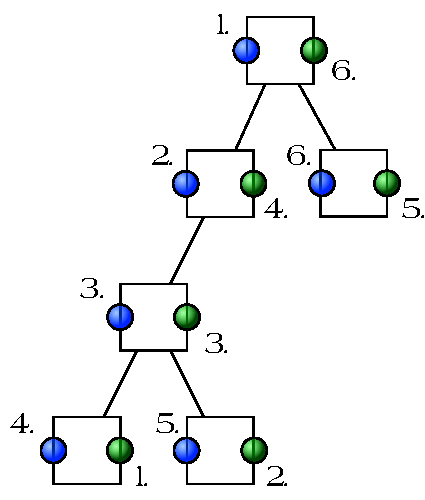
\includegraphics[width=0.4\linewidth]{traversal_mode.pdf}
 \caption{An illustration of the pre- and post-order traversal strategies: the blue points show the order in which the tree gets transformed in pre-order traversal, and the green ones illustrate the post-order traversal. Instead of pre- and post-order, we can also think of the transformations being applied top-down or bottom-up, hence the $\downarrow$ and $\uparrow$ aliases.}
 \label{figure:traversal_mode}
\end{figure}

As a first example, let us write and use a transformation that replaces all trees in the AST which do not have a range position with the \src{EmptyTree}.

\begin{lstlisting}
val tree: Tree = %\ldots%

val emptyTree = transformation[Tree, Tree] {
  case t if t.pos.isRange => t
  case _ => EmptyTree
}

preorder(allChildren(emptyTree)) apply tree
\end{lstlisting}

Preorder traversal already applies the transformation to all children, so we can simplify this to:

\begin{lstlisting}
preorder(emptyTree) apply tree
\end{lstlisting}

Of course, this is not the only way to achieve this, here is a variation that separates the testing for the range position into a predicate and uses a simple transformation to replace the tree. If the tree has a range position, it is not transformed (remember that the \src{id} transformation simply returns its argument unchanged). In case the predicate fails, the tree is replaced.

\begin{lstlisting}
val hasRangePosition = predicate((t: Tree) => t.pos.isRange)

val emptyTree = transformation[Tree, Tree] {
  case _ => EmptyTree
}

preorder(hasRangePosition &> id[Tree] |> emptyTree) apply tree
\end{lstlisting}

Using the \src{not} combinator, we can swap the two actions:

\begin{lstlisting}
preorder(not(hasRangePosition) &> emptyTree |> id[Tree]) apply tree
\end{lstlisting}

To get rid of the \src{id} transformation, we can use a different traversal strategy for the children:

\begin{lstlisting}
preorder(matchingChildren(not(hasRangePosition) &> emptyTree)) apply tree
\end{lstlisting}

More examples can be found in Section \vref{subsection:tree-transformations}.

\subsection{Creating Trees}

Most refactorings do not just reuse existing trees but also have to create new ones. The Scala compiler already contains several facilities to create new trees: the trait \src{scala.tools.nsc.ast.Trees} contains many methods that create AST trees and there's even a DSL in \src{scala.tools.nsc.ast.TreeDSL} whose ``goal is that the code generating code should look a lot like the code it generates'' \cite{TreeDSL}.

An example from \src{Trees} shows how many methods there are to create method definitions (this code has obviously been written before Scala had default arguments):

\begin{lstlisting}
def DefDef(sym: Symbol, mods: Modifiers, vparamss: List[List[ValDef]], rhs: Tree): DefDef

def DefDef(sym: Symbol, vparamss: List[List[ValDef]], rhs: Tree): DefDef
  
def DefDef(sym: Symbol, mods: Modifiers, rhs: Tree): DefDef

def DefDef(sym: Symbol, rhs: Tree): DefDef

def DefDef(sym: Symbol, rhs: List[List[Symbol]] => Tree): DefDef
\end{lstlisting}

Using the TreeDSL allows one to write very concise code. The following listing creates the AST for the code that checks whether \src{tree} is null.

\begin{lstlisting}
IF (tree MEMBER_== NULL) THEN %\ldots% ELSE %\ldots%
\end{lstlisting}

Unfortunately, all these tree construction helpers are problematic for us: they can change the position of the trees, which we have to avoid when we want to retain the source code layout. For this reason, the refactorings do not make use of these facilities but simply create the trees from scratch. There are some helper methods in \src{transformation.TreeFactory} which take care of constructing trees that are needed by the currently implemented refactorings:

\begin{lstlisting}
def mkRenamedSymTree(t: SymTree, name: String): SymTree

def mkReturn(s: List[Symbol]): Tree

def mkValDef(name: String, rhs: Tree): ValDef

def mkCallDefDef(name: String, arguments: List[List[Symbol]], 
  returns: List[Symbol]): Tree

def mkDefDef(mods: Modifiers, name: String, 
  parameters: List[List[Symbol]], body: List[Tree]): DefDef

def mkBlock(trees: List[Tree]): Block
\end{lstlisting}

Now that we have seen how trees can be transformed and how new trees can be generated, we are ready for a larger example.

\subsection{Tree Transformations}\label{subsection:tree-transformations}

For the usage in the refactoring, the \src{TreeTransformations} trait implements the traversal for Scala's AST and provides some definitions that make writing transformations more concise:

\begin{lstlisting}
def transform(f: PartialFunction[Tree, Tree]) = transformation(f)
  
def filter(f: %$\Rightarrow$% PartialFunction[Tree, Boolean]) = predicate(f)
\end{lstlisting}

Let us now take a look at a larger example: Extract Method. At the beginning of this section, we looked at the different transformations that occur during the refactoring: Insert a new method with the extracted statements and replace them with a call to this new method. This can be achieved with the following transformations:

\begin{lstlisting}
val replaceBlockOfStatements = transform {
  case block @ BlockExtractor(stats) => {
    mkBlock(stats.replaceSequence(selectedTrees, callExtractedMethod))
  }
}

val replaceSingleExpression = transform {
    case t if t == selectedTree => callExtractedMethod
}

val replace = topdown {
  matchingChildren {
    if(extractSingleTree)
      replaceSingleExpression
    else
      replaceBlockOfStatements
  }
}

val insertExtractedMethod = transform {
  case tpl @ Template(_, _, body) => 
    tpl copy (body = body ::: extractedMethod :: Nil) setPos tpl.pos
}
\end{lstlisting}

A remark on the call to \src{setPos tpl.pos} in \src{insertExtractedMethod}: Because the structure of a tree is immutable, we cannot change a tree in-place, even though we often want to do this. The source regeneration uses the position information of the trees to determine whether a tree's existing source code can be reused. So if we want a tree to appear modified in-place, we simply assign it the position of the original tree. Note that this does only work if the two trees are of the same type.

Next we need two filters that find the enclosing class' template and the method we extract from:

\begin{lstlisting}
val findTemplate = filter {
  case Template(_, _, body) => body exists (_ == selectedMethod)
}

val findMethod = filter {
  case d: DefDef => d == selectedMethod
}
\end{lstlisting}

Now we can combine these to assemble a new transformation that performs the following steps:

\begin{enumerate}
 \item Traverse the tree until the selected template is found, the one that contains \src{selectedMethod}.
 \item Once we found the template, start the following two transformations:
  \begin{enumerate}
        \item Find the method we extract from and apply the \src{replace} transformation on it.
        \item Insert the new method in the class template.
       \end{enumerate}
\end{enumerate}

%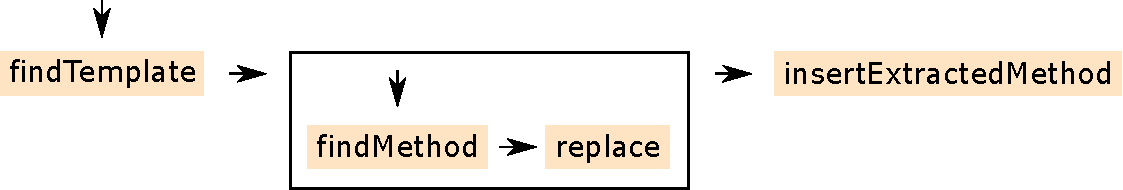
\includegraphics[width=\linewidth]{extract_method_transformation.pdf}

All these steps can be expressed with a simple transformation:

\begin{lstlisting}
val extractMethod = topdown {
  matchingChildren {
    findTemplate &> 
    topdown {
      matchingChildren {
	findMethod &> replace
      }
    } &> 
    insertExtractedMethod
  }
}
\end{lstlisting}

\section{Source Generation}\label{section:source-generation}

Once our abstract syntax tree has been refactored, we need to convert it back into its textual source code representation. This process comprises two main steps: the \textit{detection of modifications} to minimize the amount of code that is regenerated and the actual \textit{source generation}.

The first step is necessary because we -- in contrast to many other refactoring implementations -- do not keep track of modifications to the AST while they are happening but reconstruct this information afterwards. This allows us to keep the transformations simpler but consequently makes the code generation more complex. This tradeoff is worthwile because we intend the library to be reused and the transformations to be implemented by third parties.

The AST after the refactoring may contain several kinds of modifications. Trees can be moved around, deleted and new trees can be introduced. From the transformations we know that trees that are moved around keep their original position information, and newly created trees have a \src{NoPosition} attribute per default. This allows us to detect changes and can later be used during source generation to preserve the layout of already existing trees. 

\subsection{Modification Detection}

The primary goal of a fine-grained modification detection is to reduce the amount of trees that are regenerated. The source generation is invoked with a list of trees from various files that all can have an arbitrary number of changed children:

\begin{lstlisting}
def createChanges(ts: List[Tree]): Iterable[Change]
\end{lstlisting}

Modification detection performs the following three steps on the input trees:

\begin{enumerate}
 \item Group all changed trees by their file.
 \item Find the top-level changed trees for each file.
 \item Detect the change-set per top-level tree.
\end{enumerate}

Top-level trees are trees that are ancestors of other changed trees. For example, the following graph shows an AST with some changed trees in green and blue:

\begin{center}
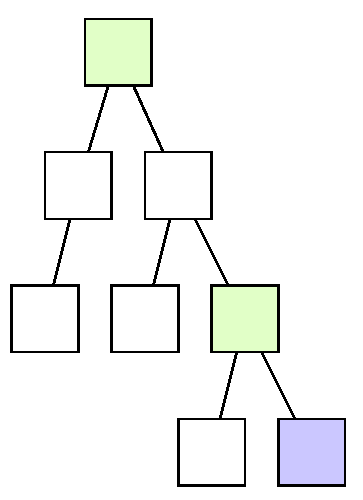
\includegraphics[width=0.2\linewidth]{ast_with_changes.pdf}
\end{center}

The \src{createChanges} method is invoked with the two green trees, but the blue tree has also been modified by a transformation.

Now if we were to generate two changes from the two green trees, we would get a problem when applying the changes because they overlap each other. The two changes would either overwrite each other or, in the case of Eclipse's Language Toolkit, yield an error. Therefore the second step of the modification detection is to find those trees that contain other changed trees. In the AST above, this would be the root node.

The third step then traverses these top-level trees and finds all changes as well as the trees that lie between changed trees, here marked in blue:

\begin{center}
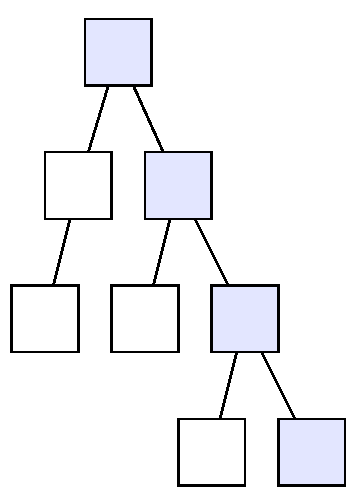
\includegraphics[width=0.2\linewidth]{ast_with_changeset.pdf}
\end{center}

This set of trees is the minimal number of trees that need to be regenerated. Trees that are not contained in the set can be kept as they are to improve the performance. \figref{figure:ast_with_changes_large} shows a larger example of the process.

\begin{figure}
 \centering
 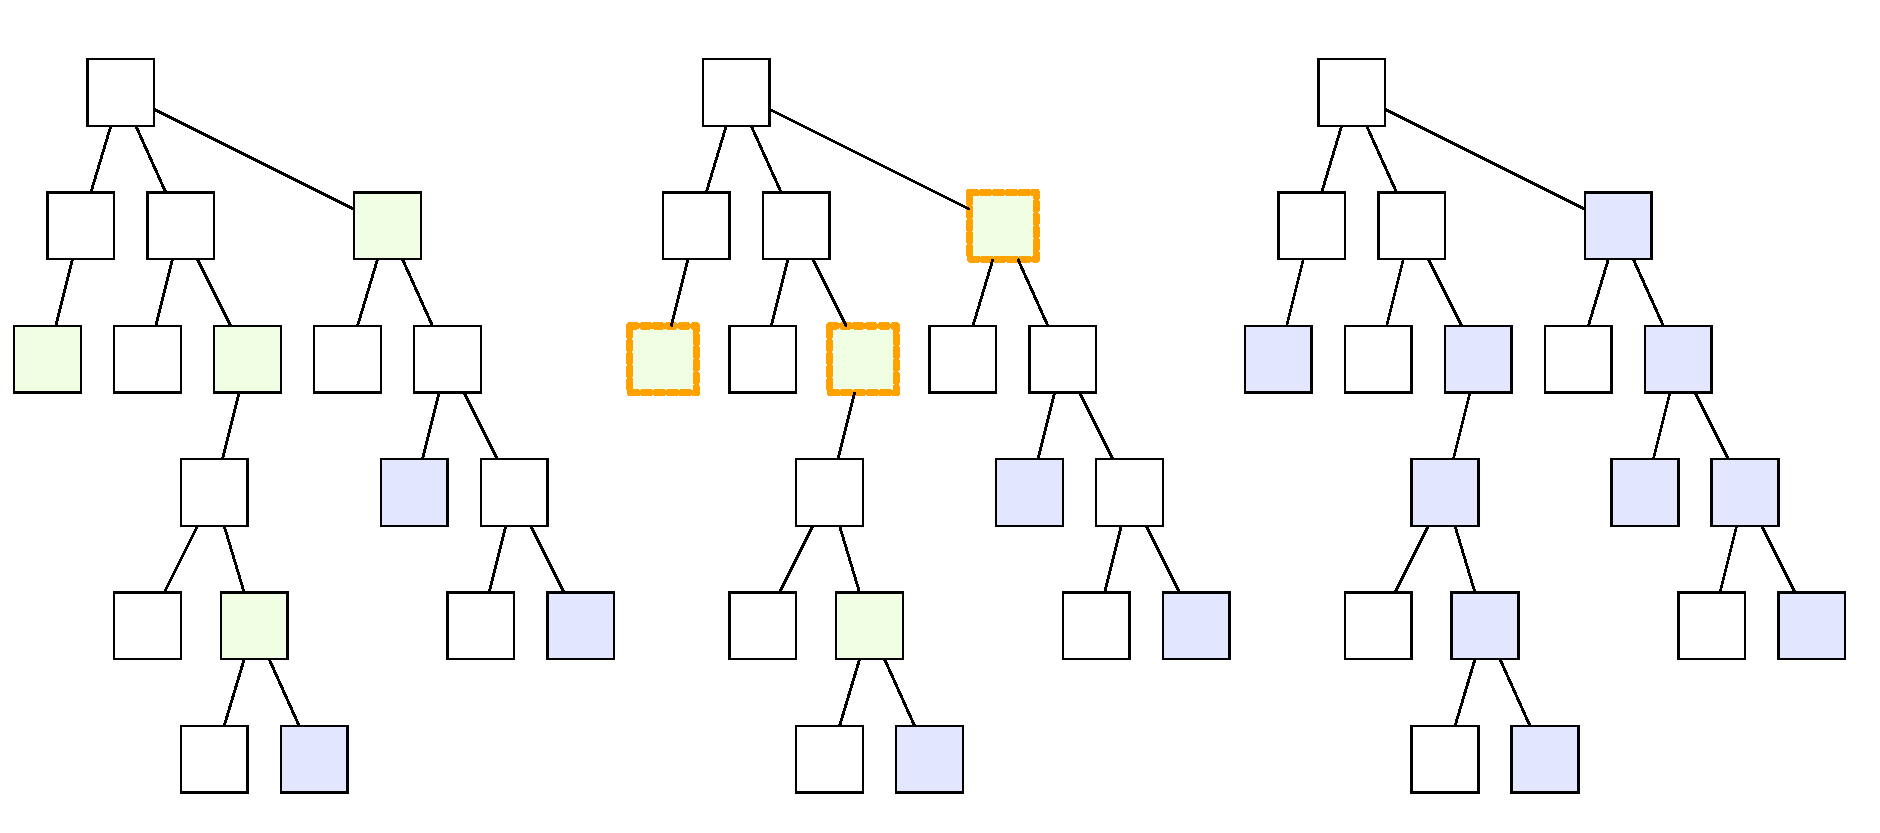
\includegraphics[width=\linewidth]{./ast_with_changes_large.pdf}
 \caption{An example of how the change set is built: the left AST shows in green the list of all trees that should be regenerated, but the blue trees have changed as well. In the middle graph, we see the trees that were identified as top-level trees. The rightmost AST shows all trees that need to be regenerated.}
 \label{figure:ast_with_changes_large}
\end{figure}

Once we have identified all top-level tree changes, we start generating source code for them. 

\subsection{Code Generation}

The AST does -- by its very nature -- not contain all the information that is necessary to fully reconstruct its original textual representation. Also, syntactic sugar of the programming language is typically not represented in the AST; only the desugared representation is preserved. An example for this are Scala's \src{for} comprehensions. Because they are equivalent with function calls to \src{map, filter, flatMap,} and \src{foreach}, there is no need to create additional tree classes for them. This means that the two statements in the following listing have the same representation in the AST.

\begin{lstlisting}
val v1 = List(1,2,3) map (i => i * 2)
val v2 = for(i <- List(1,2,3)) yield i * 2
\end{lstlisting}

Other things that are not mentioned explicitly in the AST are parenthesis, commas and many other tokens. In the context of source generation, we will call them layout elements, or just \textit{layout}. 

If we were only interested in a semantically equivalent program, we could simply pretty print the AST to generate the source code. A purely AST based pretty printer would unknowingly convert the user's \src{for} comprehensions from above into the \src{map} form. No user of a refactoring tool would accept this, and this is also not the only problem: because comments in the source code are generally considered whitespace by parsers, they are not represented in the AST and get lost during pretty printing (see \cite{RetainingComments} for a detailed treatment of this particular problem). It is clear that we need a more refined technique.

The original source code is always available to the refactoring tool, and with the position information on the trees, we have a means to look up the original source code for a tree.

Other refactoring tools (e.g. the C++ Development Tooling for Eclipse \cite{CdtOopsla} or the Ruby Development Tools \cite{RubyOopsla}) have used various approaches to solve this problem (XX ref to old doku). For some cases -- for example in a rename refactoring -- it might even be acceptable to pretty print the code as long as only very small regions of the program change. This approach can be problematic -- for example with the Extract Method refactoring, where arbitrary large parts of the program are moved around. A tool can handle this situation by cut-and-pasting the body of the extracted method. This is not feasible for us because we need a generic way to handle all kinds of unforseeable changes to the source code.

\subsubsection{Preserving Layout}

Our approach is based on using two different kinds of source printers: one that pretty prints code  and another one that reuses the existing code where possible. The \textit{pretty printer} simply prints the code with a default layout and is used for trees that were introduced during the transformation. The \textit{reusing printer} takes the existing layout with the help of the trees's position information and also makes sure all needed layout elements are present. How this is done will be explained in more detail later.

The source generation algorithm then alternates between these two printers during the code generation process.

Now we just need to know how we can reuse the existing layout. What we need is a way to decide how all these layout elements can be associated to their enclosing trees. If we take a look at the following listing, we can see several occurences of whitespace and other layout, like the three comments and the braces.

\begin{lstlisting}
package p //TODO
// myclass
class MyClass(a: Int /* the int */) {
}
\end{lstlisting}

Because no rules of the programming language dictate how the layout is associated with the other parts of the program, we have to guess how to divide it and associate it with its surrounding trees. Often this can be done by taking the types of the adjacent trees into consideration and then divide the layout according to some rules and regular expressions. 

For example, one rule says that the layout between two enclosing value definitions is split by a comma, or by newline if there is no comma present. So when the values are part of an argument list, they will get comma-separated, and if they are definitions, the layout will be split at the end of the line, so that the first value will get all layout that follows on its line. Comments can be handled with the same rules as well: a comment on a preceding and otherwise empty line is associated with the following tree.

Let us take a look at a concrete example. \figref{figure:ast_with_layout} shows the AST of the previous listing and how the layout elements have been associated with the left and right sides of a tree. Note that the \src{class} and \src{package} keywords are also considered layout, this is because they are not represented in the AST with their own tree and position information.

\begin{figure}
 \centering
 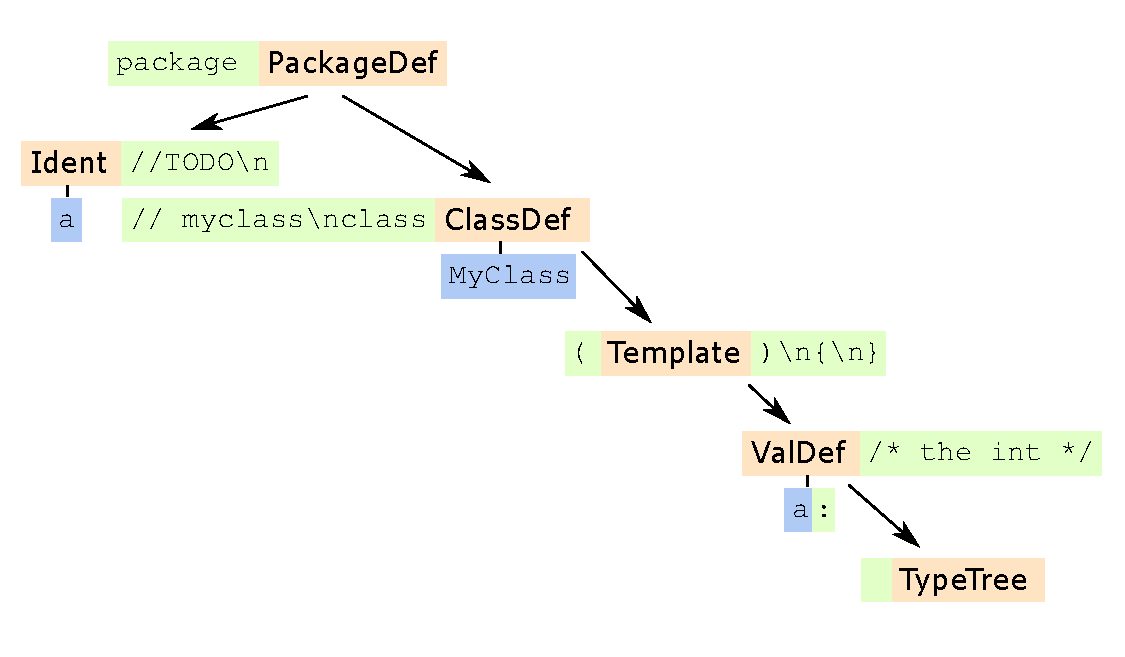
\includegraphics[width=0.8\linewidth]{ast_with_layout.pdf}
 \caption{An example of how layout can be associated with trees: the apricot colored boxes represent the trees and the green ones their associated layout. The blue parts are not real AST nodes but names; they are treated like trees in the source generation.}
 \label{figure:ast_with_layout}
\end{figure}

Once we have identified the layout that belongs to a tree, we can use it during the source generation. For example, it should be clear now that when we would delete the \src{ValDef} parameter in the above AST, then the comment would be removed along with it.

Another issue that concerns both the pretty and the reusing printer is the indentation of the code. When a new statement in a block of other statements is inserted, we want it to have the same indentation as its siblings. For this, the printers also keep track of the currently desired indentation as specified by the parent tree. 

Whether we can reuse existing code or have to invoke the pretty printed needs to be decided for each tree in the AST. This gives us the following definition of the various source printers:

\begin{lstlisting}
trait AbstractPrinter {
  def print(t: Tree, ind: Indentation): Fragment
}

trait PrettyPrinter extends AbstractPrinter {
  def print %\ldots%
}

trait ReusingPrinter extends AbstractPrinter {
  def print %\ldots%
}

trait SourceGenerator extends PrettyPrinter with ReusingPrinter {
  override def print(t: Tree, i: Indentation): Fragment = {
    if(t.hasExistingCode)
      super[ReusingPrinter].print(t, i)
    else if(t.hasNoCode)
      super[PrettyPrinter].print(t, i)
    else
      EmptyFragment
  }
%\ldots%
\end{lstlisting}

\subsubsection{Fragments and Layout}

The result of a printing operation is not a plain string but an instance of \src{Fragment}. A fragment contains a leading, center, and trailing layout. A layout is simply a wrapper around a string or a part of the source file with some additional helper methods. For example, in \figref{figure:ast_with_layout}, all the apricot and blue colored boxes are fragments and the green ones are instances of \src{Layout}.

The fragments and layouts are created in the printers, where they pattern match on the tree and recursively print the children of a tree. This is an excerpt from the pretty printer:

\begin{lstlisting}
def print(t: Tree, ind: Indentation) = t match {
  case PackageDef(pid, stats) =>
    Layout("package ") ++ 
      printTree(pid, after = newline) ++ 
      printTrees(stats, separator = newline)
%\ldots%
\end{lstlisting}

The \src{++} operation on the layout and the fragments simply concatenate their operands, again yielding a fragment. So far, we could also have just used plain Strings and concatenate them with \src{+}, except that using strings weakens the typesystem because every object can be concatenated to a String using the implicit \src{toString} method.

\subsubsection{Reusing Layout}

The printers also have to take care that all the necessary layout is printed when needed. This can become difficult when layout is reused. Imagine the following scenario: We create a new \src{Block} (a \src{Block} tree wraps a list of other statements) and insert several statements into it. The pretty printer separates each statement in a block with a newline, so the code to pretty print a block could look like this:

\begin{lstlisting}
case Block(stats) =>
  Layout("{"+newline) ++ 
    printTree(stats, separator = newline) ++ 
    Layout(newline+"}")
\end{lstlisting}

This works fine as long as the statements are not reused trees that might already have a leading or trailing newline in their associated layout. If this is the case, we could get too many blank lines between our statements. 

To solve this, the pretty printer could print the block's children one by one and then check if the newline is already present or needs to be inserted. This is tedious to do in every place where a layout element is inserted, so we need a more generic way to handle such cases, and this is where the \src{Requisites} come into play. Instead of specifying the layout directly, the printers simply declare that there needs to be a newline present in the surrounding layout:

\begin{lstlisting}
case Block(stats) =>
  Requisite("{"+newline) ++ 
    printTree(stats, separator = Requisite(newline)) ++ 
    Requisite(newline+"}")
\end{lstlisting}

Now during the concatenation of fragments and layout objects with \src{++}, it is checked whether a certain requisite is already satisfied. The layout is only generated when it is nedeed.

This leads us to the following three interfaces (the \src{++} operators and some other methods have been omitted) that are used to represent the source code in the printers:

\begin{lstlisting}
trait Layout {
  def asText: String
}

trait Requisite {  
  def isRequired(l: Layout, r: Layout): Boolean
  def apply(l: Layout, r: Layout): Layout
}

trait Fragment {
  def leading:  Layout
  def center:   Layout
  def trailing: Layout
  
  def pre: Requisite
  def post: Requisite
  
  def asText: String
}
\end{lstlisting}

Using implicit conversions (XX anhang), short aliases for the print methods and Scala's named and defaul arguments, this allows us to write the code for the two printers in a very concise way. Pattern matching gives us the ability to easily handle special cases and variations, as can be seen from the \src{Bind} matches below:

\begin{lstlisting}
trait PrettyPrinter  {
  
  def print %\ldots%  

    case Alternative(trees) =>
      p(trees, separator = " | ")
      
    case Star(elem) =>
      p(elem) ++ Layout("*")
      
    case Bind(name, body: Typed) =>
      Layout(name.toString) ++ p(body, before = ": ")

    case Bind(name, body: Bind) =>
      Layout(name.toString) ++ p(body, before = " @ \\(", after = "\\)")
      
    case Bind(name, body) =>
      Layout(name.toString) ++ p(body, before = " @ ")
    %\ldots%
}
\end{lstlisting}

\subsection{Using the Source Generator}

For users of the code generation, there are several methods to transform a tree back into source code. The \src{createChanges} method of the \src{SourceGenerator} trait creates the change objects from a list of trees by first narrowing down the changed trees and then generating the code for them:

\begin{lstlisting}
def createChanges(ts: List[Tree]): List[Change]
\end{lstlisting}

The result is a list of change objects that describe which parts in a file are to be replaced:

\begin{lstlisting}
case class Change(file: AbstractFile, from: Int, to: Int, text: String)
\end{lstlisting}

This is the preferred method for IDEs that operate with change objects. The \src{Change} object contains a useful function that applies a list of changes to a source code string:

\begin{lstlisting}
def applyChanges(ch: List[Change], source: String): String
\end{lstlisting}

Alternatively, if one just wants to generate the source code from a tree, the \src{createFragment} method can also be invoked directly. 

\begin{lstlisting}
def createFragment(t: Tree): Fragment
\end{lstlisting}


\chapter{Implemented Refactorings} \label{chapter:implemented-refactorings}

The previous chapter explained the internals of the Scala Refactoring library; in this chapter, we shall take a look at the refactorings that have so far been implemented on top of the library. 

The three components of the refactoring library -- analysis, transformation, and source generation -- can be used independently from each other, but they also have dependencies expressed through self type annotations (see \vref{section:self-type-annotation}). 

The \src{Refactoring} trait combines the library with their dependencies and can be used as an entry point by library users.

\begin{lstlisting}
trait Refactoring extends 
  Selections with 
  TreeTransformations with 
  SilentTracing with 
  SourceGenerator with 
  PimpedTrees {
  %\ldots%
}
\end{lstlisting}

Performing a refactoring is not a single-step process: when the user invokes a refactoring, the first step is to check whether the refactoring can be applied -- for example, to perform a renaming, a name has to be selected. We call this the \textit{prepare} step. This step usually has a result, which is used in a configuration dialog to parameterize the refactoring. In our renaming example, this is the new name. Using the information from the preparation step and the configured parameters, the refactoring can then be \textit{performed}. This yields either a list of changes to be applied or it can also fail. See  \figref{figure:refactoring-sequence} for a visualization.

These steps are represented by the abstract class \src{MultiStageRefactoring}, which is subclassed by all concrete refactoring implementations:
\needspace{15\baselineskip}
\begin{lstlisting}
abstract class MultiStageRefactoring extends Refactoring {
  
  type PreparationResult
  
  case class PreparationError(cause: String)

  def prepare(s: Selection): Either[PreparationError, PreparationResult]

  type RefactoringParameters
  
  case class RefactoringError(cause: String)
  
  def perform(selection: Selection, prepared: PreparationResult, params: RefactoringParameters)
    : Either[RefactoringError, List[Change]]
}
\end{lstlisting}

The reason why the selection and the preparation results need to be passed to \src{perform} is to keep it stateless. This makes it much easier for an IDE to let the user go backwards and forwards in its wizard, testing different configurations.

The remainder of this chapter introduces each refactoring and explains the current implementation for the Eclipse Scala IDE with examples. 

\section{Rename}

Renaming is one of the most used refactorings among Eclipse using Java programmers (see \cite{RefactoringStudy}, \cite{RefactoringInEclipse}). Choosing good names is a very basic and yet important task for a programmer if he wants to write readable code. During the evolution of a program, the roles of the classes, methods and variables change. Having an automated refactoring for renaming considerably reduces the cost of keeping these names in sync with their functionality.

\subsection{Features}

This implementation supports renaming of all identifiers that occur in the program -- for example, local values and variables, method definitions and parameters, class fields, variable bindings in pattern matches, classes, objects, traits, packages, and types parameters.

The IDE implementation distinguishes between two different modes: inline renaming as shown in \figref{figure:rename-screenshot-1} and the traditional dialog based implementation in \figref{figure:rename-screenshot-2}. Inline renaming is implemented using Eclipse's linked mode user interface \cite{LinkedUI}.

\begin{figure}
  \centering
  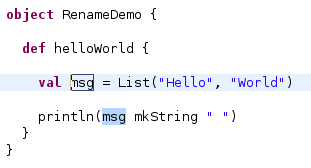
\includegraphics[width=0.5\linewidth]{rename_screenshot_1.png}
  \caption{The Rename refactoring in the inline mode: the selected name along with all references can be renamed without the need of a wizard and without previewing the changes.}
  \label{figure:rename-screenshot-1}
\end{figure}

\begin{figure}
  \centering
  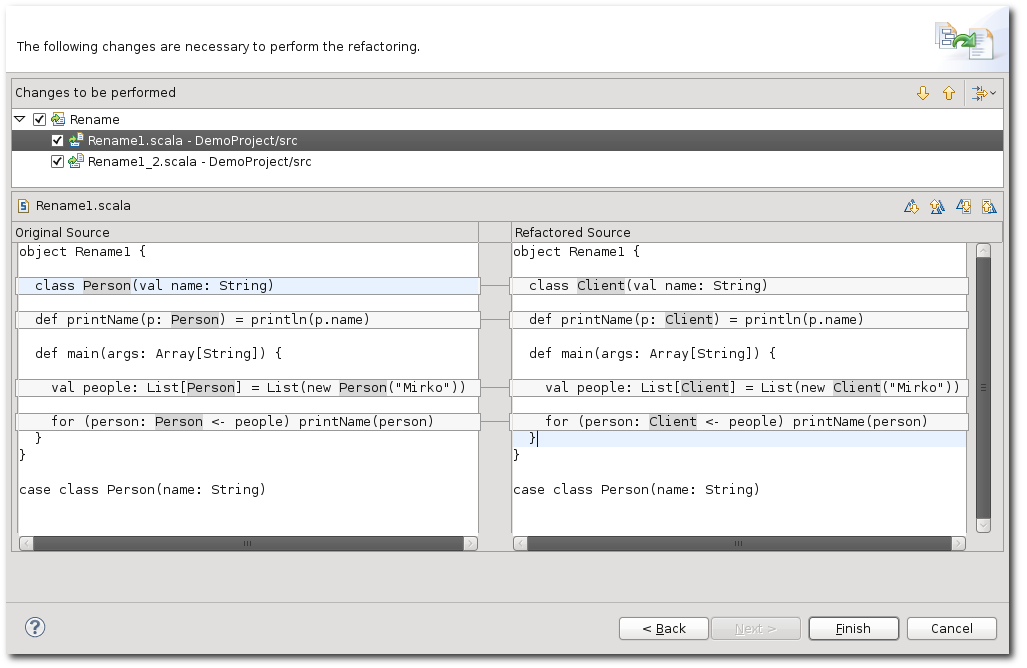
\includegraphics[width=\linewidth]{rename_screenshot_2.png}
  \caption{A classical Rename refactoring: All occurrences of the selected name are changed across all files in the project.}
  \label{figure:rename-screenshot-2}
\end{figure}

Inline renaming is automatically chosen if the identifier that is renamed has only a local scope -- for example, a local variable. All names that can potentially be accessed from other compilation units in the program are renamed with the wizard and show a preview of the changes.

\subsection{Implementation Details}

From the refactoring developer's point of view, the Rename refactoring is a quite different beast than other refactorings. Because renaming does not change the shape of the AST at all, the transformations and source generation steps are trivial. On the other hand, having an accurate index is crucial; the inline rename refactoring uses the index to find the locations of the names and does not use the source generator or tree transformations.

The implementation for the non-inline mode looks as follows:

\begin{lstlisting}
val occurences = index.occurences(prepared.selectedTree.symbol) 
    
val isInTheIndex = filter {
  case t: Tree %$\Rightarrow$% occurences contains t 
}

val renameTree = transform {
  case t: ImportSelectorTree %$\Rightarrow$% 
    mkRenamedImportTree(t, params.newName)
  case s: SymTree %$\Rightarrow$% 
    mkRenamedSymTree(s, params.newName)
  case t: TypeTree %$\Rightarrow$% 
    mkRenamedTypeTree(t, params.newName, prepared.selectedTree.symbol)
}

val rename = topdown(isInTheIndex &> renameTree |> id)

val renamedTrees = occurences flatMap (rename(_))
\end{lstlisting}

The \src{renameTree} transformation handles different kinds of trees but delegates to the \src{TreeFactory} to create the renamed trees. The \src{rename} transformation traverses the trees and renames the trees that are in the index, or keeps the original trees otherwise. This transformation is then applied to all trees returned by the index.

Why do we have to traverse the trees, would it not suffice to call \src{occurrences flatMap (renameTree(\_))} directly? No, this will not work for recursive method calls, where the method definition also has a child tree that has to be renamed.

\subsection{Limitations}

There is currently one limitation with the Rename refactoring: named parameters will not be renamed because they are not represented in the AST.

\section{Organize Imports}

It can be debated whether Organize Imports really deserves the label Refactoring, because it does not change the structure of your code; but neither does the Rename refactoring. But Organize Imports is definitely useful, therefore we chose to include it under the refactorings.

During the lifetime of a compilation unit, external dependencies can change and new import statements are added and old ones are removed. Organize imports reorders and simplifies these statements.

\subsection{Features}

Organize imports is the only implemented refactoring that does not need a configuration. The current implementation of Organize Imports performs these three steps:

\begin{description}
  \item[Sort] the statements alphabetically by their full name.
\begin{multicols}{2}
\begin{lstlisting}
import java.lang.{String, Object}
import java.io.File
import collection.mutable.ListBuffer
\end{lstlisting}
\begin{lstlisting}
import collection.mutable.ListBuffer
import java.io.File
import java.lang.{String, Object}
\end{lstlisting}
\end{multicols}

  \item[Collapse] multiple distinct imports from the same package into a single statement:
\begin{multicols}{2}
\begin{lstlisting}
import java.lang.String
import java.lang.Object
\end{lstlisting}
\begin{lstlisting}
import java.lang.{Object, String}

\end{lstlisting}
\end{multicols}

  \item[Simplify] the imports: when a wildcard imports the whole package content, individual import from that package are removed, unless they contain renames:
\begin{multicols}{2}
\begin{lstlisting}
import java.io._
import java.lang._
import java.io.FileSet
import java.lang.{String %$\Rightarrow$% S}
\end{lstlisting}
\needspace{\baselineskip}
\begin{lstlisting}
import java.io._
import java.lang.{String %$\Rightarrow$% S, _}


\end{lstlisting}
\end{multicols}
\end{description}

\figref{figure:organize-screenshot-1} shows a screenshot of the refactoring in action.

\begin{figure}
  \centering
  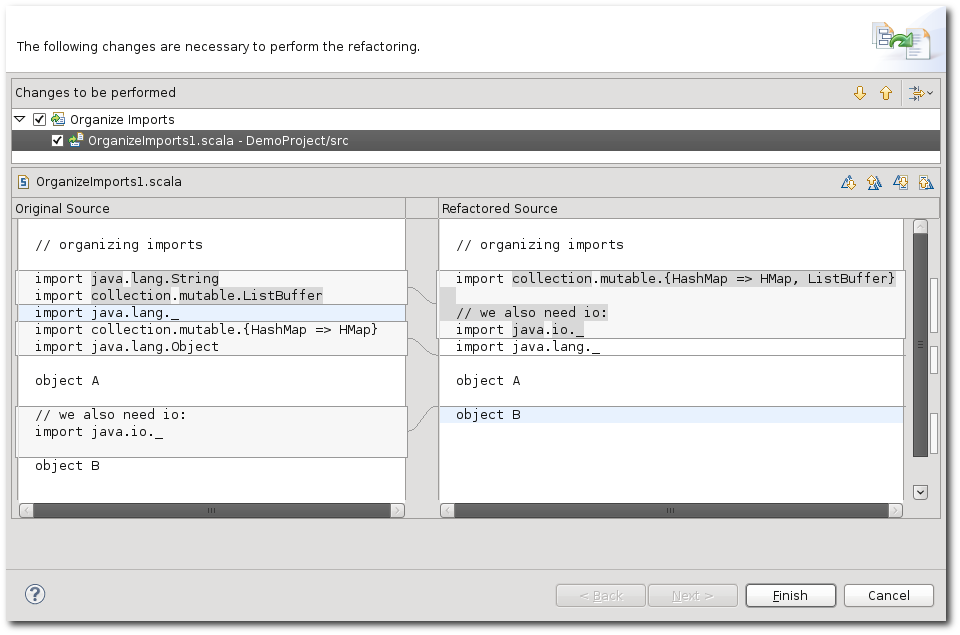
\includegraphics[width=\linewidth]{organize_screenshot_1.png}
  \caption{The Organize Imports refactoring: we can see that the imports that were scattered all over the file are now all at the top in alphabetic order. All superfluous statements are getting removed, and imports from the same package are collapsed.}
  \label{figure:organize-screenshot-1}
\end{figure}

\subsection{Limitations}

The current implementation has some limitations compared to its Java counterpart. The refactoring does not do any dependency analysis, imports that are missing are not added, and unneeded imports are not being removed by Organize Imports. There are more features that could be added in future versions:

\paragraph{Save Action} In Eclipse, actions can be performed automatically when a file is saved. Enabling Organize Imports to automatically organize the imports might be useful.

\paragraph{Introduce Import} In Scala, just as in Java, members from other packages do not have to be imported, they can also be used with their fully qualified name. Organize Imports could be extended to replace these fully qualified names with an import statement. 

\paragraph{Expand Wildcards} Once the refactoring does analyze the actually needed dependencies of the compilation unit, the refactoring might also replace all wildcard imports with just the necessary imports. This would also match the JDT's current behavior.

\paragraph{Shorten Import Paths} In contrast to Java, packages in Scala can be nested (see Appendix~\vref{section:package-nesting}). Organize Imports could take advantage of this and shorten the imported names. For example, the following import on the left could be simplified to the one on the right:

\begin{multicols}{2}
\begin{lstlisting}
package scala.tools.refactoring
package common

import scala.tools.refactoring.analysis.Index
\end{lstlisting}
\needspace{\baselineskip}
\begin{lstlisting}
package scala.tools.refactoring
package common

import analysis.Index
\end{lstlisting}
\end{multicols}

\section{Extract Local}

Extract Local Variable, also known as \textit{Introduce Explaining Variable}, should according to Fowler \cite{FowlerRefactoring} be used whenever ``you have a complicated expression''; and the proposed fix is to 

\begin{quotation}
put the result of the expression, or parts of the expression, in a temporary variable with a name that explains the purpose.
\end{quotation}

In Scala, another reason why one would want to introduce new local variables is because existing Java debuggers are easier to use when one can step over single lines and examine the resulting values.

\subsection{Features}

From a selected expression, the Extract Local refactoring will create a new value in the closest scope and replace the selected expression with a reference to that value. Just as the rename refactoring in a local scope, Extract Local also uses Eclipse's linked mode to avoid distracting the user with dialogs (see \figref{figure:extract-local-screenshot-1} for a screenshot).

\begin{figure}
  \centering
  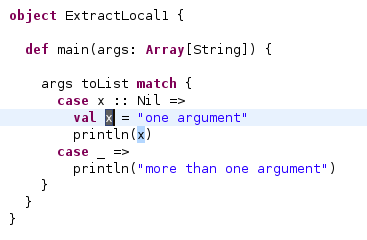
\includegraphics[width=0.5\linewidth]{extract_local_screenshot_1.png}
  \caption{The Extract Local refactoring also uses the linked mode, making extracting a local variable much faster than with a wizard.}
  \label{figure:extract-local-screenshot-1}
\end{figure}


The following listings show a few examples of the refactoring, on the left is the original code with the selection in blue, and on the right is the refactored code (line breaks were added by the author).

\begin{multicols}{2}
\begin{lstlisting}
def main(args: Array[String]) {

  println("Detecting OS..")
  val props = System.getProperties
  


  if(%\bluebox{props.get("os.name") == "Linux"}%) {
    println("We're on Linux!")
  } else
    println("We're not on Linux!")
}
\end{lstlisting}
\begin{lstlisting}
def main(args: Array[String]) {

  println("Detecting OS..")
  val props = System.getProperties
  val %\bluebox{isLinux}% = 
    props.get("os.name") == "Linux"
  
  if(%\bluebox{isLinux}%) {
    println("We're on Linux!")
  } else
    println("We're not on Linux!")
}
\end{lstlisting}
\end{multicols}

\needspace{5\baselineskip}
\begin{multicols}{2}
\begin{lstlisting}
if(props.get("os.name") == "Linux") {

  println(%\bluebox{"We're on Linux!"}%)
} else
  println("We're not on Linux!")
\end{lstlisting}
\begin{lstlisting}
if(props.get("os.name") == "Linux") {
  val %\bluebox{msg}% = "We're on Linux!"
  println(%\bluebox{msg}%)
} else
  println("We're not on Linux!")
\end{lstlisting}
\end{multicols}

A more interesting examples shows what happens if there are no curly braces around the scope:

\begin{multicols}{2}
\begin{lstlisting}
if(props.get("os.name") == "Linux") {
  println("We're on Linux!")
} else

  println(%\bluebox{"We're not on Linux!"}%)

\end{lstlisting}
\begin{lstlisting}
if(props.get("os.name") == "Linux") {
  println("We're on Linux!")
} else {
  val %\bluebox{msg}% = "We're not on Linux!"
  println(%\bluebox{msg}%)
}
\end{lstlisting}
\end{multicols}

We can extract all kinds of expressions -- for example, a part of a chain of expressions:

\begin{multicols}{2}
\begin{lstlisting}
val l = List(1,2,3)

%\bluebox{l filter (\_ \% 2 == 0)}% mkString ", "
\end{lstlisting}
\begin{lstlisting}
val l = List(1,2,3) 
val %\bluebox{filtered}% = l filter (_ %\%% 2 == 0)
%\bluebox{filtered}% mkString ", "
\end{lstlisting}
\end{multicols}

In the examples so far, we have only extracted expressions that resulted in a non-function value. Extract Local also lets you extract a method, which is turned into a partially applied function:

\begin{multicols}{2}
\begin{lstlisting}
val l = List(1,2,3)
%\bluebox{l filter}% (_ %\%% 2 == 0) mkString ", "

\end{lstlisting}
\begin{lstlisting}
val l = List(1,2,3) 
val %\bluebox{filterList}% = l filter _
%\bluebox{filterList}%(_ %\%% 2 == 0) mkString ", "
\end{lstlisting}
\end{multicols}

In the last example, we show how the extraction behaves inside single-expression statements:

\begin{multicols}{2}
\begin{lstlisting}
val l = List(1,2,3)
l filter (i %$\Rightarrow$% %\bluebox{i \% 2}% == 0) mkString ", "



\end{lstlisting}
\begin{lstlisting}
val l = List(1,2,3) 
l filter (i %$\Rightarrow$% {
  val %\bluebox{x}% = i %\%% 2 
  %\bluebox{x}%== 0
}) mkString ", "
\end{lstlisting}
\end{multicols}

\subsection{Implementation Details}

On the first glance, extracting a local variable seems to be trivial, but when braces are missing, the source generation has to work hard to create them where necessary. An additional difficulty coming from Scala's AST is that \src{Block} trees around a scope are only created when there are multiple statements present. To illustrate this, the following three listings show their respective AST.

\begin{multicols}{3}

\begin{lstlisting}
def m() = 42



\end{lstlisting}
\begin{center}
  $\Downarrow$
\end{center}
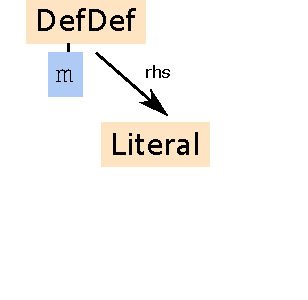
\includegraphics[width=0.9\linewidth]{defdef_without_block.pdf}

\columnbreak

\begin{lstlisting}
def m() = { 
  42
}

\end{lstlisting}

\begin{center}
  $\Downarrow$
\end{center}
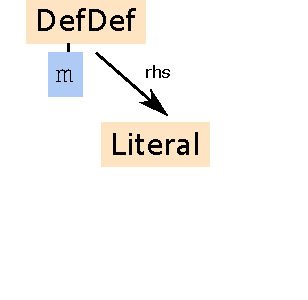
\includegraphics[width=0.9\linewidth]{defdef_without_block.pdf}

\columnbreak

\begin{lstlisting}
def m() = { 
  42
  42
}
\end{lstlisting}

\begin{center}
  $\Downarrow$
\end{center}
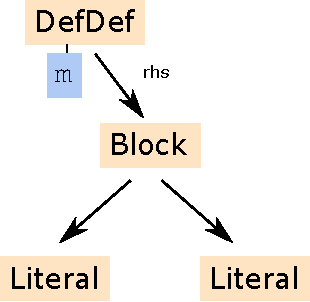
\includegraphics[width=0.9\linewidth]{defdef_with_block.pdf}
\end{multicols}

We can see that the AST in the middle looks just like the first one, even though the literal is surrounded with curly braces. Adding a second statement obviously forces the parser to surround them with a \src{Block}. When we extract a local variable, the refactoring generates a surrounding \src{Block} tree if needed, and the source generators have then to figure out whether they need to print new curly braces.
\newpage
The Extract Local transformation is implemented as follows:

\begin{lstlisting}
val findInsertionPoint = predicate((t: Tree) %$\Rightarrow$% t == insertionPoint)

def replaceTree(from: Tree, to: Tree) = 
  topdown(matchingChildren(predicate((t: Tree) %$\Rightarrow$% t == from) &> constant(to)))

val insertNewVal = transform {

  case t @ CaseDef(_, _, NoBlock(body)) %$\Rightarrow$%
    t copy (body = mkBlock(newVal :: body :: Nil)) replaces t
    
  case t @ Try(NoBlock(block), _, _) %$\Rightarrow$%
    t copy (block = mkBlock(newVal :: block :: Nil)) replaces t
    
  case t @ DefDef(_, _, _, _, _, NoBlock(rhs)) %$\Rightarrow$%
    t copy (rhs = mkBlock(newVal :: rhs :: Nil)) replaces t
    
  %\ldots%
}

val extractLocal = 
  topdown(
    matchingChildren(
      findInsertionPoint &> 
      replaceTree(selectedExpression, extractedValueReference) &>
      insertNewVal))
\end{lstlisting}

\subsection{Limitations}

Curly braces are not always placed ideally -- for example, the refactoring generates code like 

\begin{lstlisting}
(i %$\Rightarrow$% {
  %\ldots%
})
\end{lstlisting}

when it could just generate the code in the simpler form:

\begin{lstlisting}
{i %$\Rightarrow$%
  %\ldots%
}
\end{lstlisting}

\section{Inline Local}

The Inline Local -- also known as Inline Temp -- refactoring is the dual to Extract Local. It can be used to eliminate a local values by replacing all references to the local value by its right hand side.

Restricting the refactoring to \src{vals} only makes the refactoring easier to implement than its Java counterpart, where local variables can be reassigned. Still, inlining a local value can change the semantics of a program if the computation of the value has side-effects.

\figref{figure:inline-local-screenshot-1} shows a screenshot of the refactoring in the Scala IDE for Eclipse.

\begin{figure}
  \centering
  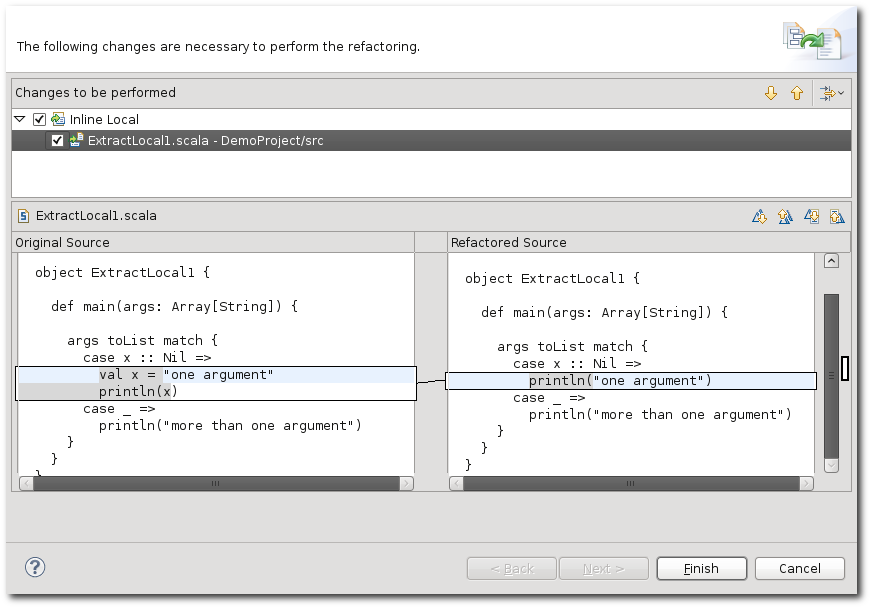
\includegraphics[width=\linewidth]{inline_local_screenshot_1.png}
  \caption{The Inline Local refactoring lets us undo the extracted local refactoring from \figref{figure:extract-local-screenshot-1}.}
  \label{figure:inline-local-screenshot-1}
\end{figure}

\subsection{Examples}

Inlining a local value is in most cases trivial, but there are a few cases where it gets more complicated. Scala allows the programmer to omit the \src{.} when calling methods in certain cases:

\needspace{8\baselineskip}
\begin{lstlisting}
scala> Console println("Hello World")
Hello World

scala> List(1,2,3) filter (_ > 1)
res1: List[Int] = List(2, 3)

scala> 42 toString
res2: java.lang.String = 42
\end{lstlisting}

Things get more complicated when such calls are chained:

\begin{lstlisting}
scala> List(1,2,3) filter (_ > 1) partition (_ %\%% 2 == 0)
res3: (List[Int], List[Int]) = (List(2),List(3))

scala> 42 toString + " is the answer"
<console>:6: error: too many arguments for method toString: ()java.lang.String

scala> (42 toString) + " is the answer"
res5: java.lang.String = 42 is the answer
\end{lstlisting}

This means that when a value is inlined, it might become necessary to add parentheses around the inlined expression, as the following examples shows:

\begin{multicols}{2}
\begin{lstlisting}
class Extr2 {
  def m {
    %\bluebox{val five = 5 toString}%;
    println(five)
    five + " is the answer"
  }
}
\end{lstlisting}
\begin{lstlisting}
class Extr2 {
  def m {

    println(5 toString)
    (5 toString) + " is the answer"
  }
}
\end{lstlisting}
\end{multicols}

This is not done by the Inline Local implementation but by the source generator; another benefit that comes from separating the source generation from the refactorings.

\subsection{Implementation Details}

The Inline Local refactoring implementation is straight forward and is assembled from two transformations: one to remove the value and another one that replaces the references to the value with its original right hand side.

The implementation for the first transformation looks as follows:

\needspace{13\baselineskip}
\begin{lstlisting}
val removeSelectedValue = {
      
  def replaceSelectedValue(ts: List[Tree]) = {
    ts replaceSequence (List(selectedValue), Nil)
  }
  
  transform {
    case tpl @ Template(_, _, stats) if stats contains selectedValue =>
      tpl.copy(body = replaceSelectedValue(stats)) replaces tpl
    case block @ BlockExtractor(stats) if stats contains selectedValue =>
      mkBlock(replaceSelectedValue(stats)) replaces block
  }
}
\end{lstlisting}

The selected value can either be contained in a block, or directly in a class template's body. To replace the reference, we first have to find out with what we want to replace it. If the value is bound to a method as follows:

\begin{lstlisting}
val inlineThis = someList filter _
\end{lstlisting}

We the \src{\_} to be removed, this is why we cannot just take the value's right hand side. The replace transformation then simply replaces all trees that reference the value:

\begin{lstlisting}
val replaceReferenceWithRhs = {
      
  val references = index references selectedValue.symbol
  
  val replacement = selectedValue.rhs match {
    // inlining `list.filter _` should not include the `_`
    case Function(vparams, Apply(fun, args)) if vparams forall (_.symbol.isSynthetic) => fun
    case t => t
  }
  
  transform {
    case t if references contains t => replacement
  }
}
\end{lstlisting}

Combining these two transformations leads to the Inline Local refactoring:
\needspace{7\baselineskip}
\begin{lstlisting}
val inlineLocal = 
  topdown(
    matchingChildren(
      removeSelectedValue &> 
      topdown(
        matchingChildren(
          replaceReferenceWithRhs))))
\end{lstlisting}


\section{Extract Method}

Also among the most used refactorings by Java programmers is Extract Method. Extract Method is another key refactoring in making code more readable: if there is some code that can be grouped together, turn it into a method, and give it a meaningful name. The refactoring takes care of passing and returning the necessary parameters.

Martin Fowler once called Extract Method the refactoring's Rubicon \cite{FowlerRubicon}: 

\begin{quotation}
if you can do Extract Method, it probably means you can go on more refactorings [because it] requires some serious work. You have to analyze the method, find any temporary variables, then figure out what to do with them.
\end{quotation} 

\subsection{Features}

There exist several variations of the refactoring depending on how the selected code interacts with surrounding local variables. In the case where no local variables are used, the refactoring is trivial, we can just move the code into its own method and insert a call at the origin. 

When local variables are used, they need to be passed into the extracted method; the problematic case arises when local variables are re-assigned or declared inside and used outside of the extracted code. In this case, the respective variable has to be returned from the created method and the call to the created method becomes an assignment to the variable. 

In Java, this scheme works as long as no more than one variable requires such special treatment. In Scala, we are also restricted by a single return value, but in contrast to Java, Scala has tuples and syntactic sugar for tuple creation and deconstruction, as shown in \figref{figure:tuple-deconstruction}. This allows us to perform the refactoring in Scala where it would not (easily) be possible with similar code in Java.

\begin{figure}
\begin{lstlisting}
def parse(source: String): (Int, String) = {
  %\ldots%
  (intResult, restSource)
}

val (parsedInt, restSource) = parse("5$")
\end{lstlisting}

\caption{An example of Scala tuples. The function \src{parseInt} has the type $String => (Int, String)$ (which is syntactic sugar for $String => Tuple2[Int, String]$). Line~3 shows how such a tuple can be returned; and the last line how it is deconstructed into the two variables \src{parsedInt} and \src{restSource}.}
\label{figure:tuple-deconstruction}
\end{figure}

Scala has other features like first class functions that allow variations of the refactoring, as described in \cite{ScalaRefactoring}. One more thing to mention is the choice of method placement: Scala allows methods to be defined inside other methods, which could also be an option for an Extract Method refactoring implementation.

\subsection{Implementation Details}

Extracting a method is done in several smaller steps:

\begin{description}
  \item[Create the Method] we want to extract. This includes determining all the inbound and outbound dependencies to construct the method signature.
  \item[Replace Extracted Statements] with a call to the newly created method. If the method returns values, we have to assign them to new local values.
  \item[Insert the Method] somewhere in the surrounding class body.
\end{description}

The transformations that are used for Extract Method have already been described in Section~\vref{subsection:tree-transformations}. A screenshot of the refactoring can be seen in \figref{figure:extract-method-screenshot-1}.

\begin{figure}
  \centering
  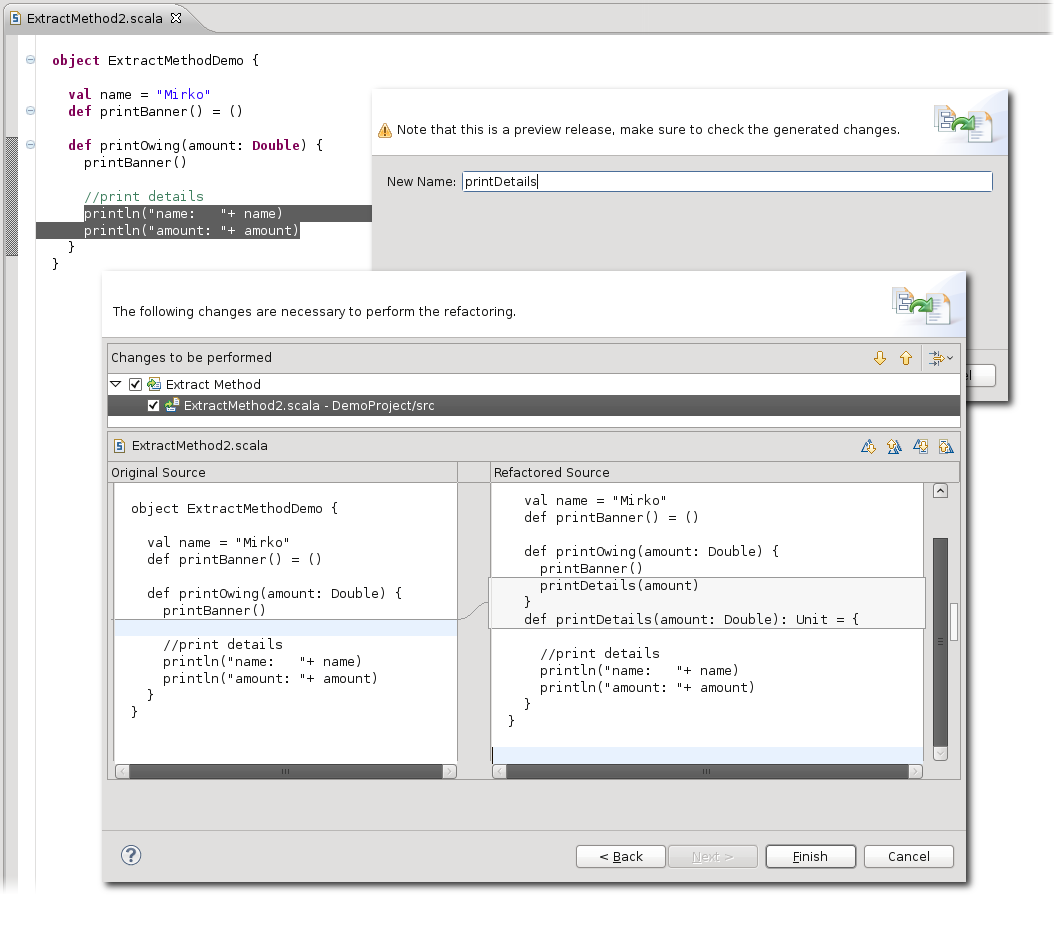
\includegraphics[width=\linewidth]{extract_method_screenshot_1.png}
  \caption{The Extract Method refactoring: starting with a text selection, the user has to provide a name for the extracted method. The proposed changes are displayed to the user and can then be applied.}
  \label{figure:extract-method-screenshot-1}
\end{figure}

\subsection{Examples}

To start, let us extract a statement that uses local variables and defines a variable that is used later in the program:

\needspace{6\baselineskip}
\begin{lstlisting}
def main(args: Array[String]) {
  println("Hello World!")
  //create a message:
   %\bluebox{val msg = args mkString ", "}%
  println(msg)
}
\end{lstlisting}

Applying the Extract Method refactoring results in a new method that takes an array as parameter and returns the created string.

\needspace{10\baselineskip}
\begin{lstlisting}
def main(args: Array[String]) {
  println("Hello World!")
  val msg = makeString(args)
  println(msg)
}
private def makeString(args: Array[String]): String = {
  //create a message:
  val msg = args mkString ", "
  msg
}
\end{lstlisting}

\subsubsection{Returning Multiple Values}

Using tuples to return values, we can return multiple values from an extracted method. The next two listings show an example:

\needspace{6\baselineskip}
\begin{lstlisting}    
def main(args: Array[String]) {
  val start =  0
  %\bluebox{val end   = 10}%
  %\bluebox{val sum = start to end reduceLeft ((x, y) => x + y)}%
  println("The sum from %\%%d to %\%%d is %\%%d".format(start, end, sum))
}
\end{lstlisting}

\needspace{10\baselineskip}
\begin{lstlisting}        
def main(args: Array[String]) {
  val start =  0
  val (end, sum) = calculateSum(start)
  println("The sum from %\%%d to %\%%d is %\%%d".format(start, end, sum))
}
private def calculateSum(start: Int): (Int, Int) = {
  val end   = 10
  val sum = start to end reduceLeft ((x, y) => x + y)
  (end, sum)
}
\end{lstlisting}

\subsubsection{Higher Order Functions}

Extract Method can also create a higher order function, as shown below:

\needspace{12\baselineskip}
\begin{lstlisting}  
def main() {
  
  val sumList: Seq[Int] => Int = _ reduceLeft (_+_)
  val prodList: Seq[Int] => Int = _ reduceLeft (_*_)
  
  val values = 1 to 10 toList
  
  %\bluebox{val     sum = sumList(values)   // the sum}%
  %\bluebox{val product = prodList(values)}%  // the product

  println("The sum from 1 to 10 is "+ sum +"; the product is "+ product)
}
\end{lstlisting}

We can now extract the calculation of the \src{sum} and the \src{product} values. Both values are returned because they are used later in the print statement (line breaks were added manually):

\needspace{17\baselineskip}
\begin{lstlisting}
def main() {
  
  val sumList: Seq[Int] => Int = _ reduceLeft (_+_)
  val prodList: Seq[Int] => Int = _ reduceLeft (_*_)
  
  val values = 1 to 10 toList
  val (sum, product) = sumAndProd(sumList, prodList, values)

  println("The sum from 1 to 10 is "+ sum +"; the product is "+ product)
}
private def sumAndProd(sumList: (Seq[Int]) => Int, 
                        prodList: (Seq[Int]) => Int, 
                        values: List[Int]): (Int, Int) = {
  val     sum = sumList(values)   // the sum
  val product = prodList(values)  // the product
  (sum, product)
}
\end{lstlisting}

\subsubsection{Arbitrary Expressions}

In our examples so far, we have only extracted statements from blocks. But we can also extract single expressions from within other expressions. The following example extracts the condition of an if-expression:

\needspace{8\baselineskip}
\begin{lstlisting}
def main(args: Array[String]) {

  println("Detecting OS..")
  
  if(%\bluebox{System.getProperties.get("os.name") == "Linux"}%) {
    println("We're on Linux!")
  }
}
\end{lstlisting}
\needspace{11\baselineskip}
\begin{lstlisting}
def main(args: Array[String]) {

  println("Detecting OS..")
  
  if(isLinux) {
    println("We're on Linux!")
  }
}
private def isLinux: Boolean = {
  System.getProperties.get("os.name") == "Linux"
}
\end{lstlisting}

\subsection{Limitations}

\begin{figure}
  \centering
  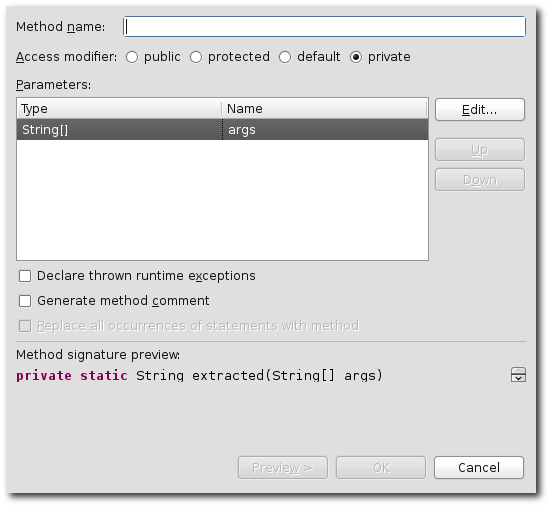
\includegraphics[width=0.6\linewidth]{extract_method_java_screenshot_1.png}
  \caption{Eclipse JDT's Extract Method Refactoring can be highly customized.}
  \label{figure:extract-method-java-screenshot-1}
\end{figure}


Compared to Eclipse's Extract Method for Java (see \figref{figure:extract-method-java-screenshot-1}), our version offers far less features -- for example, one cannot reorder the parameters, nor rename them. Allowing the user to choose where the extracted method should be placed also has not been implemented yet, and the visibility of the extracted method is always set to private.

Also, the generated code is not always as simple as it could be. Consider the following example:

\needspace{5\baselineskip}
\begin{lstlisting}
private def makeString(args: Array[String]): String = {
  //create a message:
  val msg = args mkString ", "
  msg
}
\end{lstlisting}

The local value \src{msg} could be inlined to get this simplified extracted method:

\needspace{5\baselineskip}
\begin{lstlisting}
private def makeString(args: Array[String]): String = {
  //create a message:
  args mkString ", "

}
\end{lstlisting}

\chapter{Tool Integration} \label{chapter:tool-integration}

In this chapter, we're going to look at how the implemented refactorings can be integrated into other software and how the current integration into the Scala IDE for Eclipse looks like.

\section{Dependencies}

The refactoring library depends only on the Scala compiler -- no third party libraries are used. But it also does not contain any user interface; for a seamless integration, this needs to be implemented by the integrating tool.

For a performant integration into IDEs, the refactoring implementations do not instantiate their own compiler to parse and type check the code. This is typically already being done by the IDE and would only lead to duplicate effort and significantly slow down the refactoring process.

To access the compilation units of a project, the \src{Refactoring} trait -- from which all implementations inherit -- has an abstract member of a compiler instance:

\begin{lstlisting}
trait Refactoring extends %\ldots% {
  val global: scala.tools.nsc.interactive.Global
  %\ldots% 
}
\end{lstlisting}

So in order to instantiate a refactoring implementation, a reference to the compiler has to be provided. How this is done for the automated tests is described in Chapter~\vref{chapter:testing}.

As explained at the beginning of Chapter~\vref{chapter:implemented-refactorings}, a refactoring is performed in several steps; \figref{figure:refactoring-sequence} visualizes the interaction between the user, the IDE and the refactoring library. The prepare and perform methods as well as the required parameters are part of the \src{MutliStageRefactoring} abstract class (see \figref{figure:package-layout}).

\begin{figure}
  \centering
  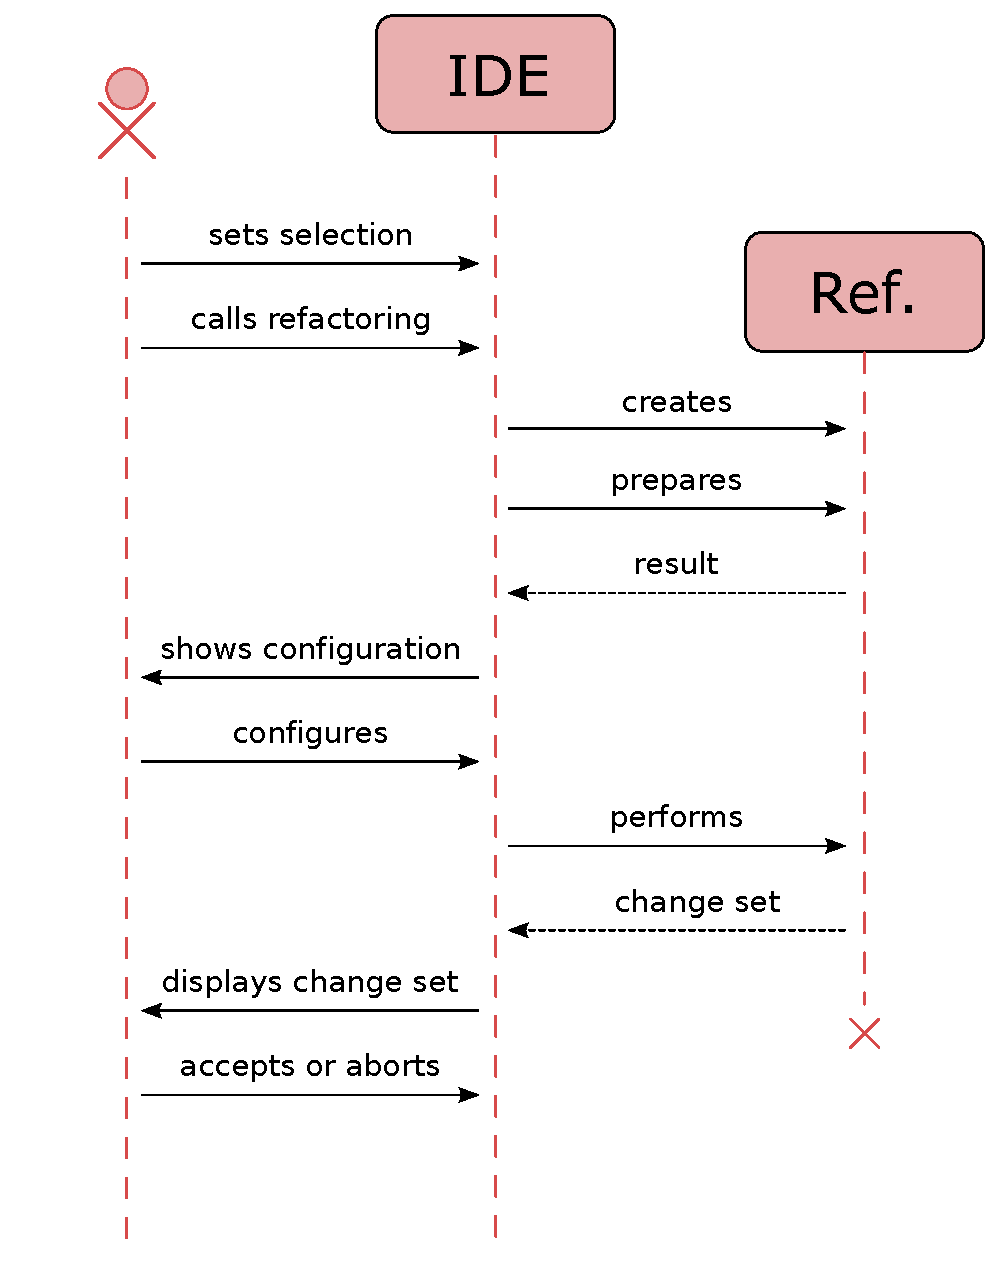
\includegraphics[width=0.9\linewidth]{refactoring-sequence.pdf}
  \caption{The simplified (error conditions are not shown) interaction that happens when a refactoring is called.}
  \label{figure:refactoring-sequence}
\end{figure}

\begin{figure}
  \centering
  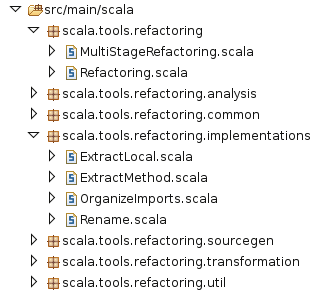
\includegraphics[width=0.5\linewidth]{package-layout.png}
  \caption{The package layout of the library, showing the base classes and the implemented refactorings.}
  \label{figure:package-layout}
\end{figure}

\section{Integrating the Library}

\begin{figure}
  \centering
  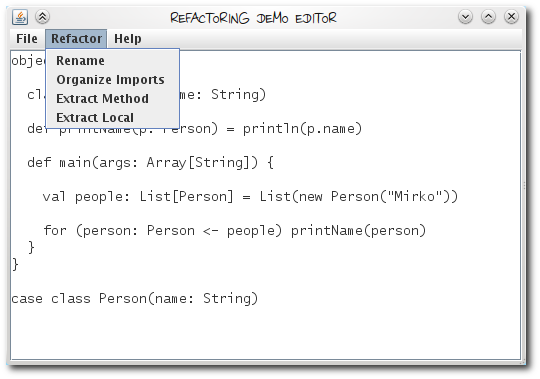
\includegraphics[width=0.7\linewidth]{refactoring-editor.png}
  \caption{The Refactoring Editor: A simple Swing editor that can open files and invoke the refactorings.}
  \label{figure:refactoring-editor}
\end{figure}

How the refactorings can be integrated will be shown on a concrete example: the Refactoring Editor shown in \figref{figure:refactoring-editor}. We show the detailed instructions for the \src{Rename} refactoring only, but others can be integrated analog. The following code is all performed in an action listener. First we have to instantiate the refactoring:

\begin{lstlisting}
val refactoring = new Rename with CompilerProvider with GlobalIndexes {
  val ast = treeFrom(editor.getText)
  val index = GlobalIndex(ast)
}
\end{lstlisting}

The compiler in this example is provided by the \src{CompilerProvider} trait, which also offers the \src{treeFrom} method to turn a \src{String} into a \src{Tree} instance. The Rename refactoring further needs an index of the whole program; we mix in the \src{GlobalIndexes} trait that allows us to construct an index from the AST (more on the index can be found in Section~\vref{section:analysis}).

Most of the refactorings need a selection to work. The \src{Selection} trait is implemented in two variations: \src{FileSelection} and \src{TreeSelection}. Depending on where the selection comes from, one or the other is easier to use. We create a \src{FileSelection} from the editor's selection:

\begin{lstlisting}
val selection: refactoring.Selection = {
  val file = refactoring.ast.pos.source.file
  val from = editor.getSelectionStart
  val to = editor.getSelectionEnd
  new refactoring.FileSelection(file, from, to)
}
\end{lstlisting}

Having a selection, we can now invoke the first refactoring step: the \src{prepare} method. Calling \src{prepare} returns \src{Either[PreparationError, PreparationResult]}, so we have to extract the result, or abort if an error occurred (a typical error cause is an unsuitable selection).

\begin{lstlisting}
val preparationResult = refactoring.prepare(selection) match {
  case Left(refactoring.PreparationError(error)) => 
    showError(error)
    return
  case Right(r) => r
}
\end{lstlisting}

The preparation result's concrete type depends on the chosen refactoring. In the case of Rename, it simply contains the tree that we want to rename. Now to perform the refactoring, we need to pass the required parameters -- the new name. The \src{askName} function of our editor opens a dialog to enter a new name.

\needspace{6\baselineskip}
\begin{lstlisting}
val refactoringParameters = {
  val selectedName = preparationResult.selectedTree.symbol.nameString
  askNewName(selectedName)
}
\end{lstlisting}

Performing the refactoring is very similar to preparing it, except that we pass more parameters and get back a list of changes on success:

\begin{lstlisting}
val changes: List[Change] = 
  refactoring.perform(selection, preparationResult, refactoringParameters) match {
    case Left(refactoring.RefactoringError(error)) => 
      showError(error)
      return
    case Right(r) => r
  }
\end{lstlisting}

In our editor, we simply apply the changes to the file, using the \src{Change.applyChanges} method. In a real editor, the user should get a chance to see the proposed changes before they are applied.

This is all that is needed to integrate the refactorings into an IDE or other editor. Most refactorings are even simpler than rename and need no configuration at all -- for example, Organize Imports or Inline Local.

Next we shall see how the refactorings have been integrated with Eclipse and the Scala IDE for Eclipse.

\section{Scala IDE for Eclipse Integration}

The Eclipse integration is of course more complex than our previous example with the Refactoring Editor. Eclipse's Java Development Tools provides a rich set of refactorings; the core of this -- the Eclipse Language Toolkit \cite{LTK} -- can be used independently of the JDT and provides common functionality -- for example, wizards that guide the user through the refactoring process, edit and change objects that represent the refactoring's outcome, a viewer to visualize the patch. The LTK also takes care of applying the changes to the source code and undo management. 

\subsection{Integrating with Eclipse LTK}

We will now take a look at how the Refactoring library has been integrated into the Scala IDE for Eclipse. The diagram in \figref{figure:eclipse-integration} gives on overview over the main classes. 

\begin{figure}
  \centering
  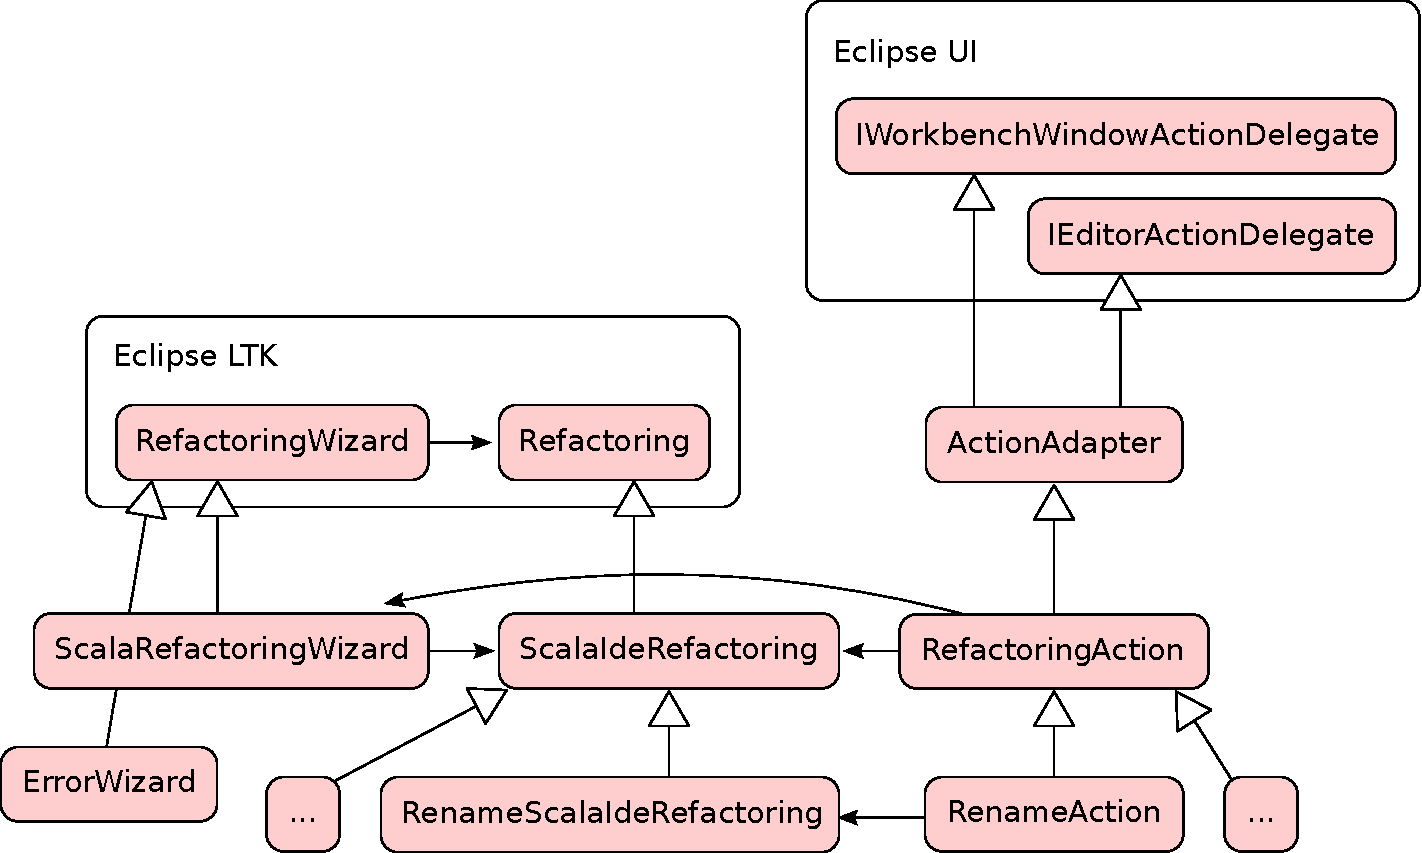
\includegraphics[width=\linewidth]{eclipse-integration.pdf}
  \caption{An overview over the integration in the Scala IDE for Eclipse; the classes that are not in boxes are part of the Scala IDE integration. The classes with ellipsis stand for the other refactorings that are implemented in the same way.}
  \label{figure:eclipse-integration}
\end{figure}

\begin{description}
  \item[ActionAdapter] unifies and simplifies the integration into Eclipse's menu bar and context menus. It provides default implementations for unused methods.
  
  \item[RefactoringAction] is the abstract driver of a refactoring execution: it is the entry point when a refactoring is executed and manages the wizards.

  \item[ScalaIdeRefactoring] serves as a bridge between the LTK and a refactoring in the library; it connects the LTK's refactoring with the library's refactorings by creating the change objects for Eclipse (these are not the same as the \src{Change} objects in the library) and checks the initial and final conditions of a refactoring, i.e. it displays the errors that can be returned by \src{prepare} and \src{perform}.
  
  \item[ScalaRefactoringWizard] wraps the \src{ScalaIdeRefactoring} in a wizard and adds pages -- for example, one page contains an input field for a new name -- from the refactoring to the wizard.
    
  \item[RenameAction] implements the \src{RefactoringAction} and contains all refactoring specific code. It instantiates the corresponding IDE refactoring -- \src{RenameScalaIdeRefactoring} -- and provides it to the generic \src{RefactoringAction}. The other refactorings are implemented analog by their respective actions.
  
  \item[RenameScalaIdeRefactoring] Adapts the Rename Refactoring from the library to the \src{ScalaIdeRefactoring} interface. An example of the \src{ExtractMethodScalaIdeRefactoring} will be shown later.
\end{description}

All these actions are hooked up to the Eclipse menus in the Scala IDE's \src{plugin.xml}.

Another member of the IDE integration is \src{EditorHelpers}. It contains additional methods that adapt some of the often used Eclipse resources to be more Scala friendly -- working with \src{Option} instead of \src{null} and higher order utility functions:

\begin{lstlisting}
object EditorHelpers {

  def activeWorkbenchWindow: Option[IWorkbenchWindow] = %\ldots%

  def activePage(w: IWorkbenchWindow): Option[IWorkbenchPage] = %\ldots%

  def activeEditor(p: IWorkbenchPage): Option[IEditorPart] = %\ldots%

  def textEditor(e: IEditorPart): Option[ScalaSourceFileEditor] = %\ldots%

  def withCurrentEditor[T](block: ScalaSourceFileEditor => Option[T]): Option[T] = %\ldots%

  def withCurrentScalaSourceFile[T](block: ScalaSourceFile => T): Option[T] = %\ldots%
}
\end{lstlisting}

\subsection{Interfacing with the Scala IDE}

As we have mentioned several times, the refactoring library needs to be given an instance of the compiler. In the Scala IDE integration, the compiler can be accessed through the \src{ScalaSourceFile}, which mixes in the \src{ScalaCompilationUnit} trait that offers the following method:

\begin{lstlisting}
trait ScalaCompilationUnit extends %\ldots%
  def withCompilerResult[T](op: ScalaPresentationCompiler.CompilerResultHolder => T): T
  %\ldots%
}
object ScalaPresentationCompiler {
  
  trait CompilerResultHolder {
    val compiler : ScalaPresentationCompiler
    val sourceFile : SourceFile
    val body : compiler.Tree
    val problems : List[IProblem]
  }
  %\ldots%
}
\end{lstlisting}

This gives us access to the underlying compiler and the parsed and type-checked tree. In the integration code, this can then be used as follows:

\begin{lstlisting}
file withCompilerResult(crh =>  %\ldots%)
\end{lstlisting}

\subsection{A Concrete Example}

To wrap up this chapter, let us take a look at a  concrete \src{ScalaIdeRefactoring} and \src{RefactoringAction} implementation. The \src{ExtractMethodAction} inherits from the \src{RefactoringAction} template method and has to implement the \src{createRefactoring} method which returns a \src{ScalaIdeRefactoring} instance:

\begin{lstlisting}
class ExtractMethodAction extends RefactoringAction {
  def createRefactoring(start: Int, end: Int, file: ScalaSourceFile) = 
    Some(new ExtractMethodScalaIdeRefactoring(start, end, file))
}
\end{lstlisting}

The \src{ExtractMethodScalaIdeRefactoring} class then adapts the library's Extract Method refactoring implementation. All the non-refactoring specific code, like calling \src{perform}, is done in \src{ScalaIdeRefactoring}.

\newpage
\begin{lstlisting}
class ExtractMethodScalaIdeRefactoring(start: Int, end: Int, file: ScalaSourceFile) 
    extends ScalaIdeRefactoring("Extract Method") {
  
  var name = ""
  
  val refactoring = file withCompilerResult { crh => 
    new ExtractMethod with GlobalIndexes with NameValidation {
      val global = crh.compiler
      val index = GlobalIndex(global.unitOfFile(crh.sourceFile.file).body)
    }
  }

  lazy val selection = createSelection(file, start, end)

  def initialCheck = refactoring.prepare(selection)
  
  def refactoringParameters = name
  
  override def getPages = 
    new NewNameWizardPage(
      s => name = s, 
      refactoring.isValidIdentifier, 
      defaultName = "extractedMethod",
      helpId = "refactoring_extract_method") :: Nil 
}
\end{lstlisting}

The \src{NewNameWizardPage} is an SWT page that asks the user for a new name (see \figref{figure:extract-local-screenshot-1} for a screenshot). The closure passed as the first parameter is called whenever the name changes, so we can update our reference. The second parameter is a function of type $String \Rightarrow Boolean$ which is used to validate the entered name. Our name-updating closure is only called when the name passes the validation. There's also a default name for the extracted method's name and a \src{helpId} parameter that is used to hook up the online help with this wizard.

The actions for refactorings that use the inline mode -- Extract Local and Rename (Local) -- override some of the \src{ScalaIdeRefactoring}'s methods to bypass the wizard and set up the linked mode user interface directly.

\subsection{Adding New Refactorings}

Integrating a new refactoring with the Scala Eclipse plug-in can be done in three steps:

\begin{enumerate}
  \item Subclass \src{ScalaIdeRefactoring} and implement the necessary methods, analog to the existing IDE refactoring implementations. Organize Imports can serve as an example for a refactoring that does not need any configuration. If configuration is necessary, Extract Method or Rename can be the adapted.
  \item Create a \src{RefactoringAction} subclass that instantiates the previously created IDE refactoring.
  \item Add the new \src{RefactoringAction} to the plugin xml. The current implementations also show how shortcuts can be registered.
\end{enumerate}

With the existing refactoring implementations as a guideline, adding a new refactoring to the Scala IDE for Eclipse should be trivial.

\chapter{Testing} \label{chapter:testing}

The necessity of automated testing in modern software projects bears no repetition. Especially with a project that is so intrinsically dependent on another component -- the Scala compiler -- and its internals, having a strong suite of integration tests is essential. 

The following chapter shows how the refactoring integration tests are implemented with the goal to provide a guide for creating new tests.

\section{Compiling Test Code}

When the refactoring implementations are used, the IDE or more generally the invoking tool provides access to the compiler. The refactoring themselves do not posses the ability to analyze the code. In the tests, we therefore also have to provide a compiler that parses and type-checks our test code.

Because instantiating and initializing the compiler is a rather expensive operation compared to running a single test, one compiler instance is shared among all the tests. The \src{CompilerProvider} trait shown below gives access to this instance and includes functionality to turn a string into a fully typed \src{Tree} instance and to add a file in the form of a string to the compiler:

\begin{lstlisting}
trait TreeCreationMethods {
  
  val global: Global
    
  def treeFrom(src: String): global.Tree = %\ldots%
  
  def addToCompiler(name: String, src: String): AbstractFile = %\ldots%
}

trait CompilerProvider extends TreeCreationMethods {

  val global = CompilerInstance.compiler
}
\end{lstlisting}

Sharing a compiler instance is not without problems: because all the compilation units end up in the same compiler, this might result in conflicts. But this can easily be avoided by putting the individual test cases into their own package.

\section{Creating a Project Layout}

Now that we have a compiler, we need a way for our tests to represent Scala source files and combine them to a project-like structure. Thanks to Scala's support for raw strings, we can embed the Scala test code directly in our test cases and do not have to store them in external files or concatenate strings together. So in our test cases we can construct an AST from a string like this:

\begin{lstlisting}
val tree: global.Tree = treeFrom("""
  object Main {
    def main(args: Array[String]) {
      println("Hello World!")
    }
  }
""")
\end{lstlisting}

The \src{FileSet} class can be used to represent a Scala test project. It has an implicit conversion (see Appendix \vref{section:implicit-conversions}) method that adds the \src{becomes} method to \src{String} so it can be used as follows:

\begin{lstlisting}
val project = new FileSet {
  """
    Content of this source file.
  """ becomes
  """
    Expected test result for this file.
  """;

  "a second source file" becomes " %\ldots% "
}
\end{lstlisting}

The \src{FileSet} class also contains a method \src{applyRefactoring} that takes a function of type $FileSet \Rightarrow List[Change]$ which \src{FileSet} uses to turn itself into a list of changes. The list of changes is then applied to the sources and their result compared to the expected results (the parameter to \src{becomes}) using the standard JUnit asserts.

\src{FileSet} class is a member of \src{TestHelper}, which extends the \src{Refactoring} trait with the compiler provider and contains some test related helper functions:

\needspace{6\baselineskip}
\begin{lstlisting}
trait TestHelper extends Refactoring with CompilerProvider {
  abstract class FileSet(val name: String) {
    %\ldots%
  }
  def findMarkedNodes(src: String, tree: global.Tree): Option[FileSelection] = %\ldots%
}
\end{lstlisting}


\section{Implementation}

Taking a look at a test for the \src{Organize Imports} refactoring, the result looks as follows:
\needspace{15\baselineskip}
\begin{lstlisting}
@Test
def sortImportsByName = new FileSet {
  """
    import scala.collection.mutable.ListBuffer
    import java.lang.Object

    object Main
  """ becomes
  """
    import java.lang.Object
    import scala.collection.mutable.ListBuffer

    object Main
  """
} applyRefactoring %\textbf{organize}%
\end{lstlisting}

The \src{organize} function simply instantiates the concrete refactoring and performs it, returning the list of changes the refactoring generated. Organize Imports is a very simple refactoring because it needs neither a selection from the user nor any other configuration. A test case for the Rename refactoring can be seen in the following listing:

\begin{lstlisting}
@Test
def renameSelfType = new FileSet {
  """
  trait /*(*/T1/*)*/

  trait T3 {
    self: T1 %$\Rightarrow$%

  }""" becomes
  """
  trait /*(*/Trait/*)*/

  trait T3 {
    self: Trait %$\Rightarrow$%

  }"""
} applyRefactoring %\textbf{renameTo}%("Trait")
\end{lstlisting}

The selection is indicated by the two comments \src{/*(*/} and \src{/*)*/}. The comments remain in the source code, this is why we also see them in the expected result. 

Now we also need a way to pass the new method's name. With the help of Scala's multiple argument lists and partial application of functions, the \src{renameTo} function can be implemented like this:

\begin{lstlisting}
def renameTo(name: String)(pro: FileSet): List[Change] = %\ldots%
\end{lstlisting}

Now the first argument -- the new name -- is applied during the test setup, and the resulting function is then passed to the \src{applyRefactoring} just like before.

\chapter{Conclusion} \label{chapter:outlook}

In this chapter, we shall review the results of this thesis and take a look at different ways the project could be continued.

\section{Accomplishments}

This thesis explored how Scala programmers can be supported with automated refactoring tools. The following achievements are worth being pointed out: 

\begin{itemize}
  \item We built an IDE independent refactoring library and integrated it into the Scala IDE for Eclipse. The library only depends on the Scala compiler and can thus be easily integrated into other IDEs and tools that manipulate Scala source code. Because the whole interaction and integration is handled by the IDE, the user does not notice that the refactorings are performed by a library. The library is currently used by the Scala IDE for Eclipse \cite{EclipseScalaIDE} and the integration is planned for the Emacs based ENSIME Scala IDE \cite{Ensime}.

  \item The following refactorings have been implemented so far: Rename, Extract Method, Extract Local, Inline Local, and Organize Imports.

  \item Creating a new refactoring does not require intimate knowledge of all parts of the library. The main task when writing a new refactoring is creating a transformation that can be applied to the Scala abstract syntax tree. To analyze the program, and index of the program symbols can be built an queried. The different parts of the library can also be used for other code manipulation tasks. For example, one project \cite{RichardEmberson} that manipulates Scala ASTs  is using the library's code generation to turn these manipulations back into source code.

  \item Refactoring transformations can easily be composed from and combined with other transformations. This allows us to build refactoring transformations from simpler, more fundamental transformations. Several different strategies can be used to apply transformations to the program.

  \item Code generation is completely hidden from the refactoring implementor. Code generation automatically detects changes in the AST and generates the code while retaining the existing formatting and comments.
\end{itemize}

The integration into the Scala IDE for Eclipse and other integrations coming up seem to indicate that the project was a success and that it is feasible to create refactoring infrastructure that is IDE independent and can be shared by several projects.

\section{Future Work}

The results of this thesis could be continued in various ways:

\begin{itemize}
  \item Creating new refactorings benefits all the IDEs that integrate the library. At the moment, only a handful of refactorings have been implemented, but a lot of work has been spent on the underlying library components. It would be interesting to see if larger refactorings can be built from the implemented simple refactoring transformations. For example, renaming the parameters during Extract Method could be implemented by applying the rename transformation to the extracted method. There are other refactorings that build on simpler ones: Form Template Method uses Extract Method. For a more detailed list, see \cite{Refactor}.

  \item One could also take the idea of user created refactorings one step further and create a graphical representation of the transformations and let the user assemble and apply them to his code. This feature could take inspiration from IntelliJ IDEA's Structural Search and Replace \cite{SSR}.

  \item Instead of creating new refactoring implementations, the existing ones could be integrated into other IDEs. For example, the NetBeans based IDE \cite{NetBeansJScalaIDE} also uses the Scala compiler, so an integration should easily be possible.

  \item The existing IDE integration could be enhanced. For example, by cross language refactorings, so that a rename in Scala would also rename the necessary Java parts of the program (see e.g. \cite{EclipseCrossLanguageRefactoring}). Alternatively, the existing integration could be improved. For example by giving the refactoring user more configuration possibilities.

  \item Not directly a continuation of this project but also interesting would be to study refactorings from functional programming languages and port them to Scala, implemented using this library. 
\end{itemize}

These ideas all assume that the library in its current state is feature complete and free of bugs, which is unlikely. So whatever course is taken, the library itself will also need to be enhanced. 

\section{Acknowledgments}

First I would like to thank my supervisor, Professor Peter Sommerlad, for his support during the thesis and for giving me a free hand in realizing my own ideas. Our weekly meetings ensured that I stayed on track and helped me manage this huge project.

Many thanks also to Miles Sabin who was always there to help me when I had any trouble with the Scala IDE and for supporting me from the beginning. 

Miguel Garcia from EPFL provided me with the Scala listings style definition and provided insightful comments on my documentation.

Many thanks to everyone from the Scala team and in the Scala community who encouraged me and provided feedback. 

A special thanks goes to Richard Emberson who uncovered many bugs in the implementation and always patiently waited for a fix.

\appendix

\chapter{Project Environment} \label{chapter:project-environment}

The project's website is located at \url{www.scala-refactoring.org}. The Git repository, wiki and issue tracker are all hosted by \textit{Assembla} and can be reached from the website. The Scala IDE for Eclipse is located at \url{www.scala-ide.org}.

The library is also published to the Scala community's central Maven repository on \url{www.scala-tools.org}, under the \src{org.scala-refactoring} group and the  \src{org.scala-refactoring.library} artifact identifier.

\section{Tools}

The following tools were used to manage and produce the almost 15'000 lines of code (including the documentation) the project contains:

\begin{description}
  \item[Scala IDE for Eclipse] is an obvious choice. A custom build was used that included the refactoring integration until it was included in the main distribution.
  \item[Eclipse Galileo] with the \textbf{Vi} plug-in.
  \item[Git] to manage the source code of the various projects and to connect to EPFL's \textbf{Subversion} repository.
  \item[Maven and Tycho] to manage the build process, which was a huge improvement compared to the older \textbf{Ant} based build.
  \item[Hudson] continuously built the project and creates update-sites for the builds.
  \item[Trac] was initially used on the project server before everything was moved to an \textbf{Assembla} space.
  \item[\LaTeXe] to create this document, along with KDE's \textbf{Kile} editor.
  \item[Inkscape and Graphviz] to create all the graphics.
\end{description}

\section{Time Report}

The mandatory work load for this thesis was 810 hours; distributed over the 21 weeks, this makes about 39 hours per week. %unterschiedlich wegen konferenzen.

\section{Project Plan}

The two project plans on the following two pages show the originally planned and the actual work that has been done. A few comments on these plans:

\begin{itemize}
  \item The original plan did not cover the whole project duration, instead it was agreed that we would assess the situation after half of the project's duration to determine the direction for the second half. 
  \item We noticed that the original plan was too ambitious, so many planned implementations could not be done. Instead, the whole source generation part had to be rewritten (see \vref{subsection:comparison-with-the-term-project} for more details on why this was necessary).
  \item The original plan contained the Scala IDE integration as one of the first tasks, but this was subsequently moved to the end because of some larger restructurings in the Scala IDE (changes of build systems). All implemented refactorings are now part of the nightly build and are going to be included in the next release.
\end{itemize}



\newpage
\thispagestyle{empty}
\begin{center}
  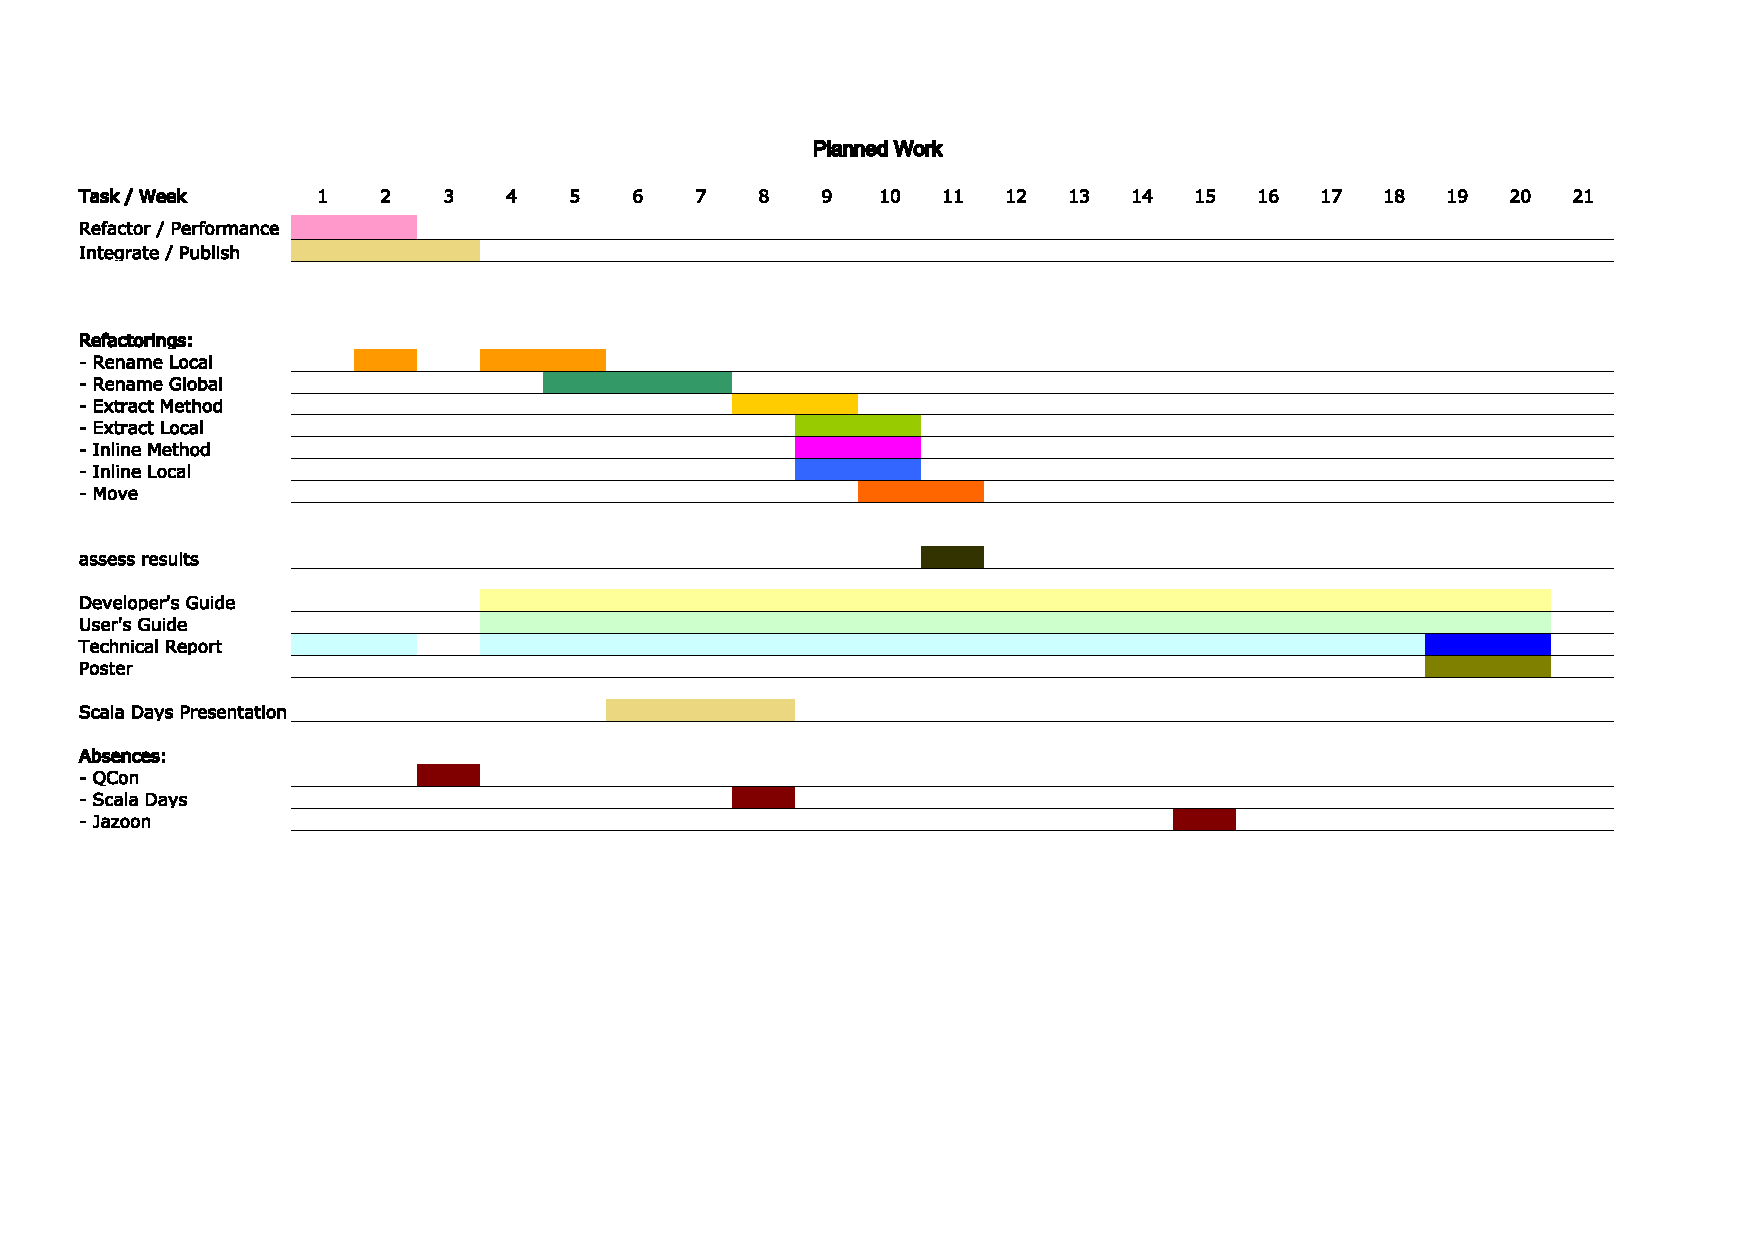
\includegraphics[width=1.7\linewidth,angle=90]{project_plan_1.pdf}
\end{center}

\newpage
\thispagestyle{empty}
\begin{center}
  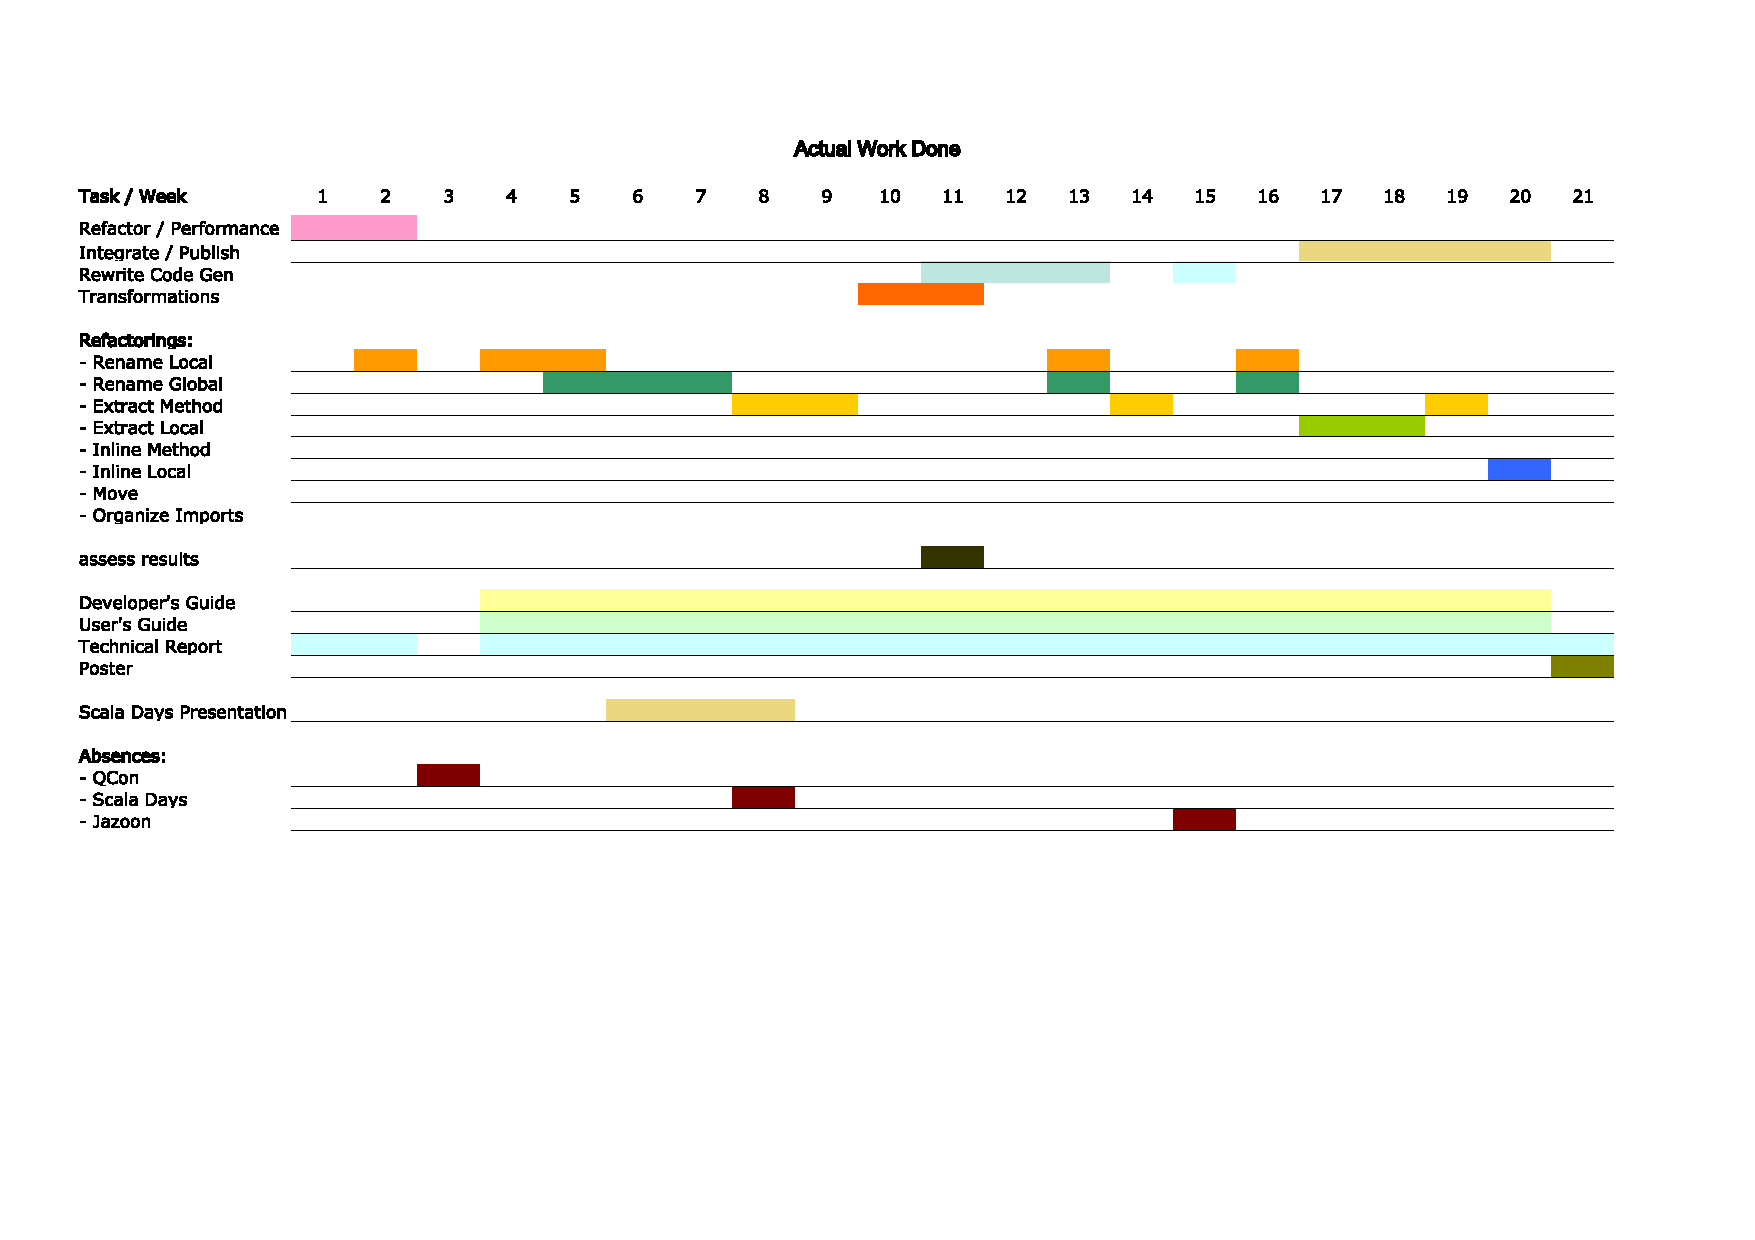
\includegraphics[width=1.7\linewidth,angle=90]{project_plan_2.pdf}
\end{center}


\chapter{User Guide} \label{chapter:user-guide}

This appendix describes the implemented refactorings from the user's perspective. We show how the refactorings can be invoked, what features and limitations they have.

The refactorings are all accessible from the Refactoring menu and with various shortcuts:

\begin{center}
  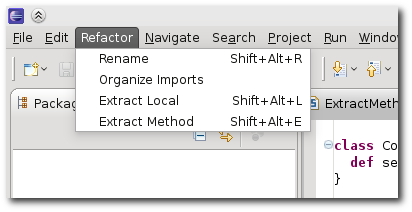
\includegraphics[width=0.6\linewidth]{refactoring-menu-screenshot.png}
\end{center}

The contents of this user guide are also included in the Scala IDE for Eclipse's online help.

\section{Rename}

The Rename refactoring can be used to rename all names defined in a Scala program. This includes for example: methods, classes, objects, local variables, method parameters, type parameters. To perform the refactoring, the name has to be selected -- placing the cursor on the name also suffices -- and then the refactoring can be invoked.

If the name that is renamed is only accessible in the source file -- for example, a local variable, or a method inside another method -- then the refactoring is invoked in the inline mode, which links all occurrences in the source file and changes them as you type:

\begin{center}
  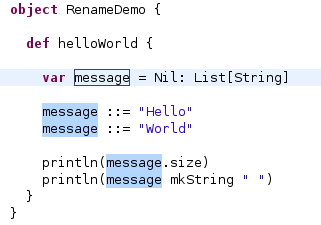
\includegraphics[width=0.5\linewidth]{rename_screenshot_3.png}
\end{center}

If the name is accessible from other source files, the renaming is done in the wizard and the changes can be previewed:

\begin{center}
  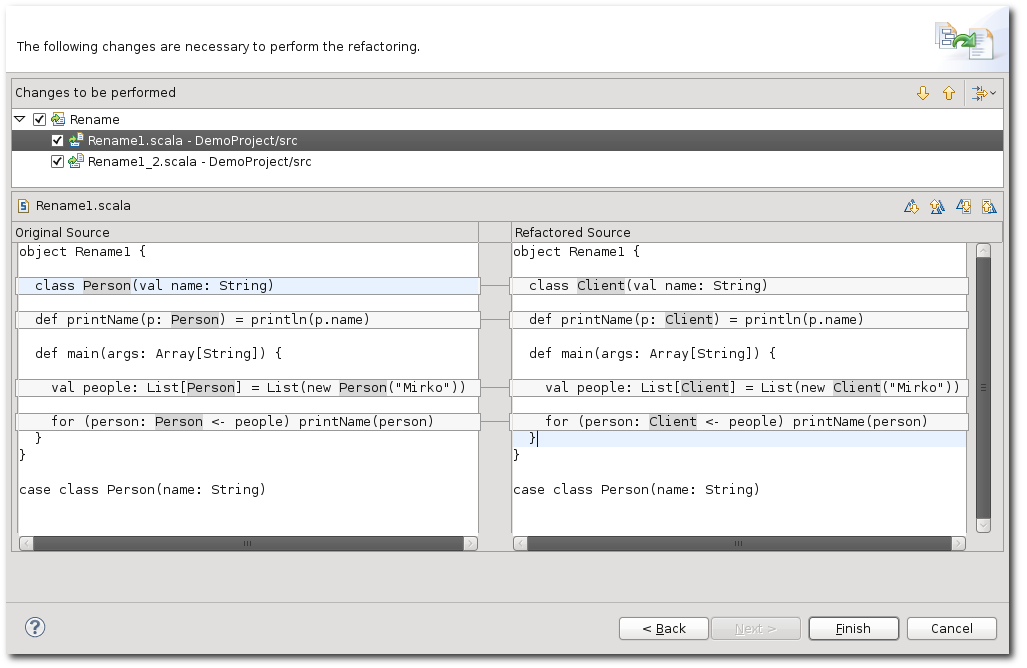
\includegraphics[width=\linewidth]{rename_screenshot_2.png}
\end{center}

When the new name is entered in the wizard, it is checked if the name is valid and not already in use.

\subsection{Limitations}

When renaming a top-level type in a file where the source file has the same name as the type, the file is currently not renamed. 

Scala 2.8 introduced named parameters, but because of how they are represented internally, they are not being renamed at the moment, leading to compile errors.

\section{Organize Imports}

Organize Imports cleans up the import statements in the current file. It does however not remove any unused imports nor imports that are needed for the program to compile. The refactoring does the following to the imports:

\begin{description}
  \item[Sorts] the statements alphabetically by their full name.
  \item[Collapses] multiple distinct imports from the same package into a single statement.
  \item[Simplifies] the imports: when a wildcard imports the whole package content, individual import from that package are removed, unless they contain renames.
\end{description}

The following screenshot shows the changes Organize Imports proposes:

\begin{center}
  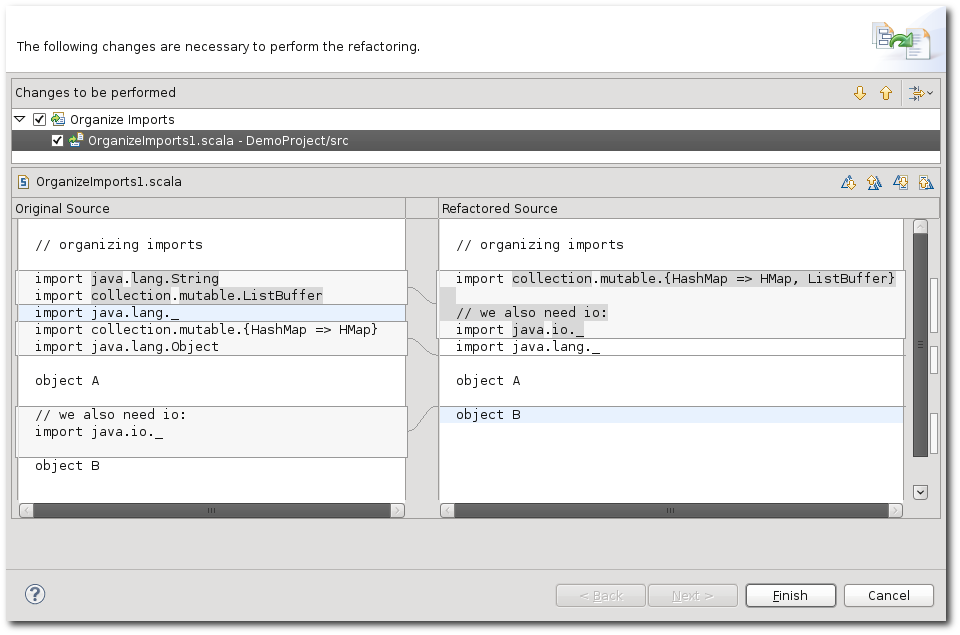
\includegraphics[width=\linewidth]{organize_screenshot_1.png}
\end{center}

\subsection{Limitations}

The current implementation has some limitations compared to its Java counterpart. The refactoring does not do any dependency analysis, imports that are missing are not added, and unneeded imports are not being removed by Organize Imports. 

\section{Extract Local}

Extract Local allows you to introduce a new local variable from an expression: the value is initialized with the selected expression and the original  expression is replaced with a reference to the new value. 

The refactoring is also known as Introduce Explaining Variable, because it allows the programmer to simplify long expressions by splitting them into several smaller ones and making the code more readable. 

Selecting an expression like in the following screenshot:

\begin{center}
  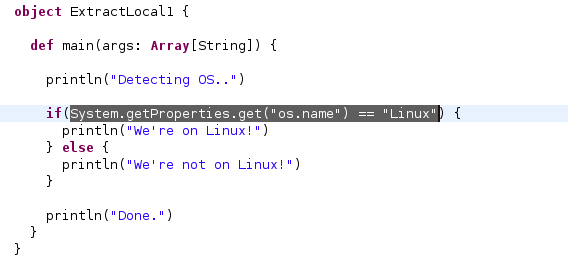
\includegraphics[width=0.8\linewidth]{extract_local_screenshot_2.png}
\end{center}

and then executing the refactoring creates a new local variable and lets you change the name in Eclipse's linked mode:

\begin{center}
  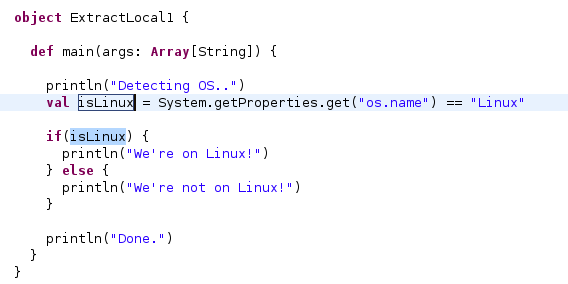
\includegraphics[width=0.8\linewidth]{extract_local_screenshot_3.png}
\end{center}

Extracting new local values can also be useful for debugging to see the intermediate results of a computation.

\section{Inline Local}

The Inline Local refactoring lets you remove unneeded local values. Selecting a value and invoking the refactoring will replace all references to the value with the value's right hand side.

Note that when there are side-effects in the evaluation of the value, the refactoring might change you program's behavior. Only local \src{vals} can be inlined, \src{vars} are not supported.

The following screenshot shows the refactoring in action:

\begin{center}
  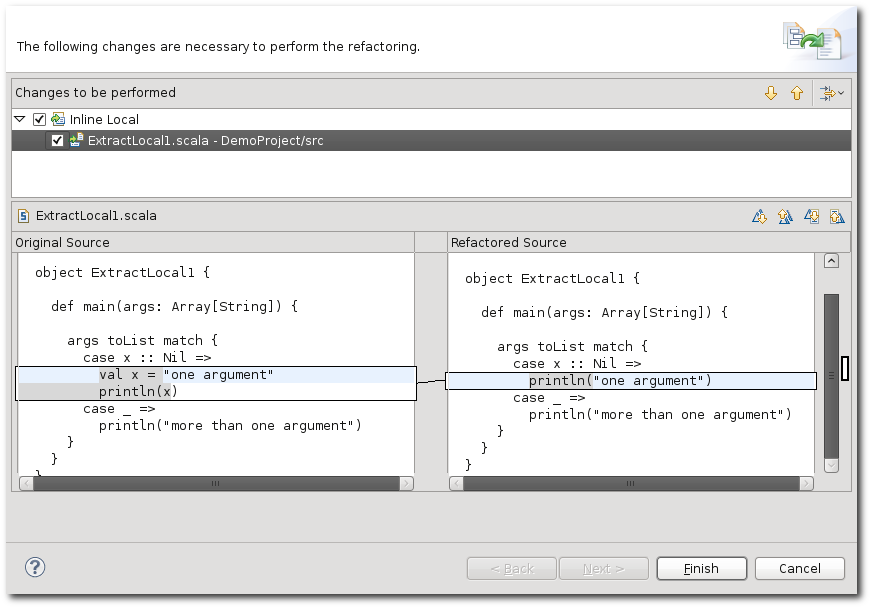
\includegraphics[width=\linewidth]{inline_local_screenshot_1.png}
\end{center}

\section{Extract Method}

The Extract Method refactoring lets you extract one or many expressions into a new private method. The refactoring takes care of passing all necessary parameters to the method and returns all values that are needed.

To invoke the refactoring, a selection inside of a method has to be made. The refactoring wizard will then ask for a new name and show a preview of the changes:

\begin{center}
  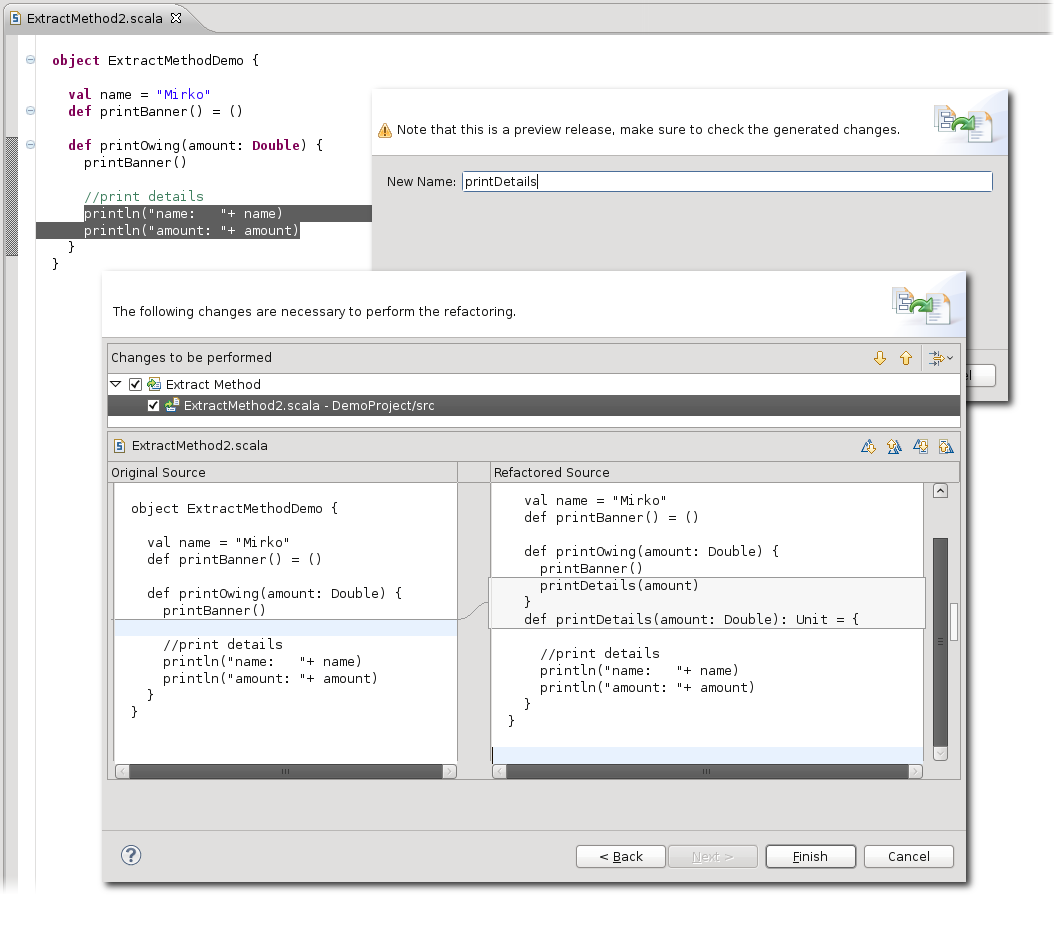
\includegraphics[width=\linewidth]{extract_method_screenshot_1.png}
\end{center}

\subsection{Limitations}

Compared to Eclipse's Extract Method for Java, the Scala version currently lacks many features -- for example, one cannot reorder the parameters, nor rename them. Allowing the user to choose where the extracted method should be placed also has not been implemented yet, and the visibility of the extracted method is always set to private.

\chapter{Developer How-To} \label{chapter:developer-how-to}

This appendix provides an introduction for developers that are interested in developing new refactorings. We will create a new refactoring step-by-step and point to the relevant sections in the main documentation for details and background information. 

%Why should anybody want to write a refactoring? IDEs usually provide a variety of general refactorings and code generators, but maybe a framework or project specific automated refactoring that no IDE offers would be helpful. 

Before we start, we should clarify that when we write about \textit{refactoring}, this includes all program transformations that affect the source code, so a transformation that just creates new code -- e.g. adds a method to a class -- can be implemented as well.

\section{Introduction}

A refactoring is essentially a transformation of the program in its abstract syntax tree form. Because our Scala programs are stored in plain text files, the transformed syntax tree has to be converted back to text -- and this without losing all our pretty formatting. 

One of the design goals of the Scala Refactoring library was to separate these two concerns as good as possible, so that the implementor of a refactoring can concentrate on transforming trees and let the library handle all the code generation for him (for more information on how the code generation works, see Section~\vref{section:source-generation}). 

To make it easier for those who already know the Scala compiler's abstract syntax tree (AST), the refactorings are completely based on this AST instead of introducing a new program representation (the Scala AST is documented in Appendix~\vref{chapter:scala-ast}). 

\section{The Example}

In Scala, the compiler generates getters and setters for us; this is great for the common case where the value is just set or retrieved. If one needs to do more -- for example validate the new value, Scala allows to write explicit getters and setters. The following listing shows the original code:

\needspace{3\baselineskip}
\begin{lstlisting}
class Person(val name: String, var age: Int) {
  def debug = name +" is "+ age +" years old."
}
\end{lstlisting}

and the same with explicit getters and setters (remember that in Scala \src{person.age = 42} is the same as \src{person.age\_=(42)}):

\needspace{5\baselineskip}
\begin{lstlisting}
class Person(name: String, private var _age: Int) {
  def debug = name +" is "+ age +" years old."
  def age = _age
  def age_=(age: Int) = _age = age
}
\end{lstlisting}

Now let us automated this! In this example, we will concentrate on the refactoring implementation only; how the integration into the IDE or an other tool could look like is explained in Chapter~\vref{chapter:tool-integration}.

To keep our example as simple as possible, the refactoring will only take two parameters: a string that represents the source code and an integer for the current caret position -- that is, the selected value or variable for which the refactoring should create explicit getters and setters. The result of this operation is another string that represents the refactoring program. 

The refactoring will have to perform the following operations:

\begin{enumerate}
  \item Find out which value the user selected.
  \item Find the class that the selected value belongs to.
  \item Create a private field for the selected value.
  \item Create the getter and the setter. The setter is only needed when the selected value is mutable.
  \item Transform the AST to include the new methods and changed field.
  \item Turn the changed AST back into source code.
\end{enumerate}

\section{Implementing It}

Refactoring implementations subclass from \src{scala.tools.refactoring.Refactoring}, which has an abstract member \src{global: scala.tools.nsc.interactive.Global} -- an instance of the compiler that is typically provided by the IDE. Because we are not implementing this example in an IDE setting, we can mix in the \src{scala.tools.refactoring.util.CompilerProvider} trait which instantiates a compiler for us.

So far, our code looks as follows:

\begin{lstlisting}
class GenerateGettersAndSettersRefactoring(sourceCode: String, caretPosition: Int) 
    extends Refactoring with CompilerProvider {
  
  import global._
  
  def refactor(): String = { %\ldots% }
}
\end{lstlisting}

In the remainder of the example, we will complete the \src{refactor} method. The first thing we need to do is to turn the \src{sourceCode} string into an AST. The \src{treeFrom} method mixed in from \src{CompilerProvider} can do this:

\begin{lstlisting}
    val ast: Tree = treeFrom(sourceCode)
\end{lstlisting}

The \src{ast} value now holds a reference to the root element of the AST. Next we want a way to find out on which \src{val} (or \src{var}) the caret is positioned, and we need to know the corresponding template (the body of the class), where we later want to insert the getters and setters. From the source file and the caret position, we can create a \src{Selection} object which contains methods to find selected trees:
    
\begin{lstlisting}
    val selection = new FileSelection(ast.pos.source.file, caretPosition, caretPosition+1)
    
    val selectedValue = selection.findSelectedOfType[ValDef].getOrElse {
      return "No val/var selected."
    }
    
    val template = selection.findSelectedOfType[Template].getOrElse {
      return "No enclosing class found."
    }

    val createSetter = selectedValue.symbol.isMutable
\end{lstlisting}

Now that we know more about the selected value, we can start creating the new trees that we are going to insert into the AST. The new private field is created by prefixing the existing one with \src{\_}. We also need to adjust the modifiers of the field:

\begin{lstlisting}
    val privateName = "_"+ publicName
    
    val privateFieldMods = if(createSetter) {
      Modifiers(Flags.PARAMACCESSOR).
        withPosition (Flags.PRIVATE, NoPosition).
        withPosition (Tokens.VAR, NoPosition)
    } else {
      Modifiers(Flags.PARAMACCESSOR)
    }
      
    val privateField = selectedValue copy (mods = privateFieldMods, name = privateName)
\end{lstlisting}

The \src{withPosition} calls make sure that the field gets \src{private var} modifiers. Modifiers serve two purposes here: they describe the role of the tree -- \textsc{\src{paramaccessor}} -- and the modifiers that need to be present in the source code -- \textsc{\src{private}} and \textsc{\src{var}}.

The getter and setter trees are simple method definitions (see Appendix~\vref{chapter:scala-ast} for more information on the AST classes):

\begin{lstlisting}
    val getter = DefDef(
        mods = Modifiers(Flags.METHOD) withPosition (Flags.METHOD, NoPosition), 
        name = publicName, 
        tparams = Nil, 
        vparamss = List(Nil), 
        tpt = EmptyTree, 
        rhs = Block(
                Ident(privateName) :: Nil, EmptyTree))
    
    val setter = DefDef(
        mods = Modifiers(Flags.METHOD) withPosition (Flags.METHOD, NoPosition), 
        name = publicName +"_=",
        tparams = Nil,
        vparamss = List(List(ValDef(Modifiers(Flags.PARAM), publicName, 
                               TypeTree(selectedValue.tpt.tpe), EmptyTree))), 
        tpt = EmptyTree,
        rhs = Block(
                Assign(
                  Ident(privateName),
                  Ident(publicName)) :: Nil, EmptyTree))
\end{lstlisting}

The \src{vparamss} argument is a list of lists, because of Scala's multiple argument lists. Note that we use the selected value's type tree for the formal parameter's \src{ValDef}. In general, one does not have to specify any types in the modified trees except when they should be printed in the source code.

The \src{rhs} of the setter is simply an assignment with the private name on the left and the public name on the right. Both \src{rhs} are wrapped in a \src{Block} to make sure the source generator prints curly brackets around the method.

Now that we have all the trees, we need to insert them into our existing AST. Modifying ASTs is done with \textit{transformations} (see Section~\vref{section:transformation}). A transformation is basically a function that takes a tree and returns an \src{Option[Tree]}. This transformation is then applied to all trees in the AST. 
\newpage
The \src{transform} function creates a transformation from a partial function and is used as follows:

\begin{lstlisting}
    val insertGetterSettersTransformation = transform {
        
      // only apply the transformation to the selected template
      case tpl: Template if tpl == template => 
      
        // find the selected value in the class body and replace it with our privateField
        val classParameters = tpl.body.map { 
          case t: ValDef if t == selectedValue => privateField setPos t.pos
          case t => t 
        }
      
        // only create a setter when we have a `var`
        val body = if(createSetter)  
          getter :: setter :: classParameters
        else
          getter :: classParameters
        
        tpl.copy(body = body) setPos tpl.pos
    }
\end{lstlisting}

Note the \src{setPos} calls: Whenever a new tree should replace an existing one -- that is, be inserted at the same position and taking over the original tree's comments -- we give it the original tree's position.

We now have a generic transformation, but it has not been applied to our AST yet. There exist different strategies on how to do this, for our transformation we traverse the tree top-down (or pre-order) and try to apply \src{insertGetterSettersTransformation} to all subtrees. If the transformation can be applied, the modified tree replaces the original one; otherwise the original tree is retained.

\begin{lstlisting}
    val transformedAst = topdown(
                           matchingChildren(
                             insertGetterSettersTransformation)) apply ast
\end{lstlisting}
    
The AST can now be transformed into a list of change objects -- i.e a patch -- that can then be applied to the source code:

\begin{lstlisting}
    val changes = refactor(transformedAst.toList)
    
    Change.applyChanges(changes, sourceCode)
\end{lstlisting}

\section{The Result}

Applying the refactoring to both attributes of our original example:

\begin{lstlisting}
class Person(val name: String, var age: Int) {
  def debug = name +" is "+ age +" years old."
}
\end{lstlisting}

yields the following result:

\needspace{12\baselineskip}
\begin{lstlisting}
class Person(_name: String, private var _age: Int) {
  def age = {
    _age
  }
  def age_=(age: Int) = {
    _age = age
  }
  def name = {
    _name
  }
  def debug = name +" is "+ age +" years old."
}
\end{lstlisting}

This concludes our example of an automated refactoring implementation. All we had to do was to create some trees and write a transformation that applied our changes to the AST; turning the AST back into source code happened almost automatically.

The implementation of this refactoring can be found in the \src{implementations} package of the library. To see how other refactorings were implemented, continue reading Chapter~\vref{chapter:implemented-refactorings}. To learn more about the internals of the library, take a look at Chapter~\vref{chapter:refactoring-library}.

\chapter{Scala AST}

This chapter describes the individual tree classes that are used in the Scala compiler. It starts with the root class \src{Tree}, some of the more interesting traits and abstract classes and then describes all concrete trees. Scala constructs -- syntactic sugar -- that are not represented as trees like parallel assignment and for-comprehensions are described in the last section.

On the right of the tree class' name are its ancestor classes and traits. All concrete trees are case classes, their parameters are listed below the class name.

\newcommand{\member} [2] {\hfill \begin{footnotesize}\src{#1} \newline \vspace{5pt} \src{#2}\end{footnotesize}\vspace{5pt}}

\section{Base Classes and Traits}

(A nice picture that shows the inheritance relations of the trees and traits)

\paragraph{Tree} \hfill \newline

\noindent The \src{Tree} class is the root of all other trees in the AST. It provides some common functionality for all other trees, for example the position (\src{\textit{pos}: Position}), the type (\src{\textit{tpe}: Type}), and the symbol (\src{\textit{symbol}: Symbol}). Not all subtrees have symbols or types, so these attributes might return \src{null}.

More operations of the \src{Tree} class are defined in \src{TreeOps}.

\paragraph{SymTree} \hfill \begin{footnotesize}\src{Tree}\end{footnotesize} \newline

\noindent The \src{SymTree} trait is extended by all trees that can have a symbol, but it returns \src{NoSymbol} by default.

\paragraph{DefTree} \hfill \begin{footnotesize}\src{SymTree <: Tree}\end{footnotesize} \newline

\noindent The \src{DefTree} class is extended by all trees that define or introduce a new entity into the program. Each \src{DefTree} also has a name and introduces a symbol.

\paragraph{RefTree} \hfill \begin{footnotesize}\src{SymTree <: Tree}\end{footnotesize} \newline

\noindent \src{RefTrees} are references to \src{DefTrees}. They also have a name and their symbol is the same as their corresponding \src{DefTree's}.

\paragraph{Symbol}

\paragraph{Position}

\paragraph{Name}

\section{Concrete Trees}

\paragraph{EmptyTree} \hfill \begin{footnotesize}\src{TermTree <: Tree}\end{footnotesize} \newline

\noindent An object that can stand in for most other trees, it has no position, no type and no symbol. For \src{ValDefs}, the equivalnt is the \src{emptyValDef} object.

\paragraph{PackageDef} \member{MemberDef <: DefTree <: SymTree <: Tree}{\textit{pid}: RefTree, \textit{stats}: List[Tree]}

\noindent Describes a package clause with a package identifier and a list of statements. The package identifier is either an instance of \src{Ident} for a package like \src{package a} or \src{Select} for a package name like \src{package a.b}. A compilation unit root is always a package, even if there is no explicit package declaration. In this case, the identifier is simply \src{<empty>}. According to the Scala Language Specification, the two different notations are equal:

\begin{multicols}{2}
\begin{lstlisting}
package a
package b.c
  
  
\end{lstlisting}

\begin{lstlisting}
package a {
  package b.c {
  }
}
\end{lstlisting}
\end{multicols}


If there exists a top level package definition, its position does not necessarily enclose the whole source file, everything that lies before the \src{package} keyword or after the last statement in the package is not contained in the position. In a package that contains no explicit package declaration and only one statement, the package definition has the same start and end position as the statement, but a different point.

\paragraph{ClassDef} \member{ImplDef <: MemberDef <: DefTree <: SymTree <: Tree}{\textit{mods}: Modifiers, \textit{name}: Name, \textit{tparams}: List[TypeDef], \textit{impl}: Template}

\noindent The definition for all kinds of classes and traits (objects are defined in \src{ModuleDef}). The definition contains all modifiers, the name and the type parameters. The class' constructor arguments, super classes and its body are all defined in the impl \src{Template}.

Modifiers are a set of \src{abstract, final, sealed, private, protected, trait, case}. The \src{class} keyword is not contained in the modifiers. If the class is anonymous (can be queried with \src{isAnonymousClass} on the class' symbol), the name is of the form \src{\$anon}.

\paragraph{ModuleDef} \member{ImplDef <: MemberDef <: DefTree <: SymTree <: Tree}{\textit{mods}: Modifiers, \textit{name}: Name, \textit{impl}: Template}

\noindent The definition of a singleton object, similar to the \src{ClassDef} except that a module does not take type parameters. 

\paragraph{Template} \member{SymTree <: Tree}{\textit{parents}: List[Tree], \textit{self}: ValDef, \textit{body}: List[Tree]}

\noindent The implementation of either a \src{ModuleDef} or \src{ClassDef}; also contains early definitions, super types, the self type annotation, and the statements in the class body. In the case of a \src{ClassDef}, it also contains the class's constructor parameters.

The following example illustrates into what constructor parameters and super constructor calls are desugared:

\begin{multicols}{2}
\begin{lstlisting}
class B(i: Int) extends A(i)





\end{lstlisting}

\begin{lstlisting}
class B extends A with ScalaObject {
  <paramaccessor> private[this] val i: Int = _
  def this(i: Int): B = {
    B.super.this(i)
  }
}
\end{lstlisting}
\end{multicols}

To identify the parameters from the list of body statements, we can check the modifiers of all \src{ValDefs} for the \src{PARAMACCESSOR} and \src{CASEACCESSOR} flags. In the same way, values and types from the early definition are identified by their \src{PRESUPER} flag. To check whether a value or type belongs to the early definitions, the compiler's \src{treeInfo.isEarlyDef} method can be used.

The super call parameters can be identified as follows: find the constructor \src{DefDef} (\src{symbol.isConstructor} is \src{true}) and then check its body \src{Block} for the following pattern: \src{Apply(Select(Super(\_, \_), \_), args)}. Because only super classes and not traits can have constructor arguments, there can be at most one such super call.

If the self type is not specified, it is the \src{emptyValDef} object. Otherwise, there are several different kinds of self type annotations:

\begin{multicols}{2}
\begin{lstlisting}
trait Trait {
}
trait ATrait {
  self =>
}
trait BTrait {
  self: ATrait =>
}
trait CTrait {
  self: BTrait with ATrait =>
}
\end{lstlisting}
\begin{lstlisting}
abstract trait Trait extends scala.AnyRef {
}
abstract trait ATrait extends scala.AnyRef { 
  self: ATrait => 
}
abstract trait BTrait extends scala.AnyRef {
  self: BTrait with ATrait =>
}
abstract trait CTrait extends scala.AnyRef {
  self: CTrait with BTrait with ATrait =>
}
\end{lstlisting}
\end{multicols}

We see that a self type annotation automatically intersects the current trait type with all explicitly named types. Extracting the exact positions of all type names is not trivial and involves searching the value's position for the occurences of the names.

It is also allowed to use \src{this} for the self type's name. This introduces no alias and the name of the \src{ValDef} is just \src{\_}.

\paragraph{ValDef} \member{ValOrDefDef <: MemberDef <: DefTree <: SymTree <: Tree}{\textit{mods}: Modifiers, \textit{name}: Name, \textit{tpt}: Tree, \textit{rhs}: Tree}

\noindent Value definitions are all definitions of \src{vals}, \src{vars} (identified by the \src{MUTABLE} flag) and parameters (identified by the \src{PARAM} flag).

The modifiers also contain the other properties a value can have: \src{override, abstract, final, implicit, lazy, private, protected}. Whether a modifier is applicable depends on the context where a value is used. A value can also be synthetic, i.e. compiler-generated (identified by the \src{SYNTHETIC} flag) -- for example in the following two equivalent statements, a synthetic value is passed to \src{println}:

\begin{lstlisting}
List(1, 2) foreach println
List(1, 2) foreach (println _)
\end{lstlisting}

Even though the value is compiler generated, it sometimes still has a name. In these examples, it is \src{x}, which is the name of \src{println}'s formal parameter. Sometimes, a name of the form \src{x\$1} is used.

Note that not every \src{val} in the source code is necessarily also represented by a \src{ValDef}. The following listing shows how the abstract value in the trait on the left is actually represented by the compiler:

\begin{multicols}{2}
\begin{lstlisting}
trait A {
  val a: Int
}
\end{lstlisting}
\begin{lstlisting}
abstract trait A extends scala.AnyRef {
  <stable> <accessor> def a: Int
}
\end{lstlisting}
\end{multicols}

In general, values are always private to the class. For external access, stable accessors are generated, as the following listing illustrates.

\begin{multicols}{2}
\begin{lstlisting}
class A {
  val a = 42

}
\end{lstlisting}
\begin{lstlisting}
class A extends Object with ScalaObject {
  private[this] val a: Int = 42;
  <stable> <accessor> def a: Int = A.this.a
}
\end{lstlisting}
\end{multicols}

Several methods defined on \src{Symbol} can be used to cross-reference between the getters, setters and their underlying value. The \src{accessed} method on a getter or setter symbol returns the underlying value's symbol. To get the corresponding setter or getter from a value, the methods \src{getter} and \src{setter} can be used.

\paragraph{DefDef} \member{ValOrDefDef <: MemberDef <: DefTree <: SymTree <: Tree}{\textit{mods}: Modifiers, \textit{name}: Name, \textit{tparams}: List[TypeDef], \textit{vparamss}: List[List[ValDef]], \textit{tpt}: Tree, \textit{rhs}: Tree}

\noindent The \src{DefDef} trees represent method definitions. Methods can have modifiers that further describe the implementation or constrain its visibility. Every method also has a name, but note that symbolic names are stored in their ASCII form, to get the original name, the symbol's \src{nameString} method can be used.

In contrast to a \src{ValDef}, a method can be parametrized with types and may have several argument lists. Each argument is represented by a \src{ValDef}.

Abstract methods have the \src{DEFERRED} flag and an \src{EmptyTree} right hand side child.

Finding methods in sub- or super classes requires the use of their \src{symbols}. Super classes can be found via the \src{ancestors} method on the class' symbol. Going into the other direction of the inheritance hierarchy is more expensive. To find all subclasses of a class $C$ one has to collect all other classes in the universe and test each's ancestors for the presence of $C$. Once the class hierarchy is assembled, the definition symbol's \src{overriddenSymbol} method can be used on each class in the hierarchy to gather all overrides.

\paragraph{TypeDef} \member{MemberDef <: DefTree <: SymTree <: Tree}{\textit{mods}: Modifiers, \textit{name}: Name, \textit{tparams}: List[TypeDef], \textit{rhs}: Tree}

\noindent \src{TypeDef} trees are definitions of types. The following listing shows three occurences -- \src{A, B, C} -- of \src{TypeDefs}:

\begin{lstlisting}
class Types {
  type A = Int
  type B >: Nothing <: AnyRef
  def d[C] ...
}
\end{lstlisting}

Just as the other member definitions trees (\src{ValDef} and \src{DefDef}), type definitions can have modifiers.

\paragraph{LabelDef} \member{DefTree <: SymTree  <: Tree $\wedge$ TermTree <: Tree}{name: Name, params: List[Ident], rhs: Tree}

\noindent %TODO

\paragraph{Import} \member{SymTree <: Tree}{\textit{expr}: Tree, \textit{selectors}: List[ImportSelector]}

\noindent An import statement imports one or many names -- the selectors -- from a package or object \src{expr}. An \src{ImportSelector} has two name-position pairs, the first one stands for the imported name and the second one is an optional renaming. Wildcard imports are also represented with an \src{ImportSelector}.

Import trees can also be comma separated, in this case, only the first import includes the \src{import} keyword in its position.

\paragraph{Block} \member{TermTree <: Tree}{\textit{stats}: List[Tree], \textit{expr}: Tree}

\noindent A \src{Block} encloses a list of statements in \src{\{ \ldots \}} and returns the value of its \src{expr} child. \src{Block} trees are only generated when neede, e.g. the right hand side of a \src{DefDef} with a single expression is not a \src{Block} but the expression itself, even when the expression is enclosed in \src{\{ \ldots \}}.

The \src{expr} is usually the last line of a block, with regards to their positions, but this is not always the case. For example, when creating an anonymous class, the class is introduced with a compiler generated name and then instantiated:

\begin{multicols}{2}
\begin{lstlisting}
val a = new {
}




\end{lstlisting}
\begin{lstlisting}
val a: java.lang.Object = {
  final class $anon extends scala.AnyRef {
    %\ldots%
  }
  new $anon()
}
\end{lstlisting}
\end{multicols}

\paragraph{CaseDef} \member{Tree}{\textit{pat}: Tree, \textit{guard}: Tree, \textit{body}: Tree}

\paragraph{Alternative} \member{TermTree <: Tree}{\textit{trees}: List[Tree]}

\paragraph{Star} \member{TermTree <: Tree}{\textit{elem}: Tree}

\paragraph{Bind} \member{DefTree <: SymTree <: Tree}{\textit{name}: Name, \textit{body}: Tree}

\paragraph{UnApply} \member{TermTree <: Tree}{\textit{fun}: Tree, \textit{args}: List[Tree]}

\paragraph{ArrayValue} \member{TermTree <: Tree}{\textit{elemtpt}: Tree, \textit{elems}: List[Tree]}

\paragraph{Function} \member{TermTree <: Tree $\wedge$ SymTree <: Tree}{vparams: List[ValDef], body: Tree}

\noindent The \src{Function} tree contains a single list of parameters and a body for the implementation. The following listing shows various usages of the \src{Function} tree and how their desugared function trees look like.

\begin{multicols}{2}
\begin{lstlisting}
list foreach println


list foreach (println _)


list foreach (i => println(i))
list foreach ((i: Int) => println(i))
list foreach {
  case i => println(i)
}
\end{lstlisting}
\begin{lstlisting}
list foreach ({
  ((x: Any) => println(x))
})
list foreach ({
  ((x: Any) => println(x))
})
list foreach (((i: Int) => println(i)))
list foreach (((i: Int) => println(i)))
list foreach (((x0$1: Int) => x0$1 match {
  case (i @ _) => println(i)
}))
\end{lstlisting}
\end{multicols}

In the first two examples, the functions are encapsulated in an additional \src{Block} (hence the curly braces). When the function parameter is not given a name explicitly, the compiler generates one and marks it with the \src{SYNTHETIC} flag. In the last of the examples, we can see that the pattern matching on the parameter is made explicit in the AST.

\paragraph{Assign} \member{TermTree <: Tree}{\textit{lhs}: Tree, \textit{rhs}: Tree}

\paragraph{If} \member{TermTree <: Tree}{\textit{cond}: Tree, \textit{thenp}: Tree, \textit{elsep}: Tree}

\noindent An \src{If} expression consists of three parts: the condition, the then part and the else part. If the else part is omitted, the literal \src{()} of type \src{Unit} is generated and the type of the conditional is set to an upper bound of \src{Unit} and the type of the then expression, usually \src{Any}.

\src{else if} terms are implemented using nested if conditionals. We can see this in the following listing.

\begin{multicols}{2}
\begin{lstlisting}
if (a)
  b
else if (c)
  d
else
  e

\end{lstlisting}
\begin{lstlisting}
if (a)
  b
else
  if (c)
    d
  else
    e
\end{lstlisting}
\end{multicols}

Note that the \src{if} used in pattern matching guards is not an \src{If} tree but a member of a \src{CaseDef} tree.

\paragraph{Match} \member{TermTree <: Tree}{\textit{selector}: Tree, \textit{cases}: List[CaseDef]}

\paragraph{Return} \member{TermTree <: Tree $\wedge$ SymTree <: Tree}{\textit{expr}: Tree}

\noindent The \src{Return} tree contains an expression that consitutes the return value. For \src{return} statements without an expression, the compiler generates a \src{()} literal.

\paragraph{Try} \member{TermTree <: Tree}{\textit{block}: Tree, \textit{catches}: List[CaseDef], \textit{finalizer}: Tree}

\paragraph{Throw} \member{TermTree <: Tree}{\textit{expr}: Tree}

\paragraph{New} \member{TermTree <: Tree}{\textit{tpt}: Tree}

\noindent The \src{New} tree represents \src{new} statements, the \src{tpt} member is the type that is being instantiated.

\paragraph{Typed} \member{TermTree <: Tree}{\textit{expr}: Tree, \textit{tpt}: Tree}

\paragraph{TypeApply} \member{GenericApply <: TermTree <: Tree}{\textit{fun}: Tree, \textit{args}: List[Tree]}

\paragraph{Apply} \member{GenericApply <: TermTree <: Tree}{\textit{fun}: Tree, \textit{args}: List[Tree]}

\paragraph{ApplyDynamic} \member{TermTree <: Tree $\wedge$ SymTree <: Tree}{\textit{qual}: Tree, \textit{args}: List[Tree]}

\paragraph{Super} \member{TermTree <: Tree $\wedge$ SymTree <: Tree}{\textit{qual}: Name, \textit{mix}: Name}

\paragraph{This} \member{TermTree <: Tree $\wedge$ SymTree <: Tree}{\textit{qual}: Name}

\paragraph{Select} \member{RefTree <: Symtree <: Tree}{\textit{qualifier}: Tree, \textit{name}: Name}

\noindent The \src{Select} tree occurs on places that select a name from a qualifier, e.g. in method calls. Note that the typer fully qualifies references as illustrated in the following listing.

\begin{multicols}{2}
\begin{lstlisting}
class A {
  val a = %\ldots%
  val b = a
}
\end{lstlisting}
\begin{lstlisting}  
class A {
  val a = %\ldots%
  val b = A.this.a
}
\end{lstlisting}
\end{multicols}

As usual, these generated trees then have an \src{OffsetPosition}.

\paragraph{Ident} \member{RefTree <: Symtree <: Tree}{\textit{name}: Name}

\noindent Holds a \src{Name}, which can be generated (check with \src{symbol.isSynthetic}) by the compiler. Note that the name is in its ASCII form; the printed name can be found via the tree's symbol.

\paragraph{Literal} \member{TermTree <: Tree}{value: Constant}

\noindent All literals are represented by \src{Literal} trees. All possible kinds of constants can be seen in the \src{Constant} trait.

\paragraph{TypeTree} \member{AbsTypeTree <: TypTree <: Tree}{\textit{original}: Tree}

\noindent From the Scala compiler's documentation: 

\begin{quote}
A synthetic term holding an arbitrary type. Not to be confused with with TypTree, the trait for trees that are only used for type trees. TypeTrees are inserted in several places, but most notably in \src{RefCheck}, where the arbitrary type trees are all replaced by TypeTrees.\end{quote}

The original type tree is still accessible via the \src{TypeTree}'s \src{original} member. Note that the standard tree \src{Traverser} and \src{Transformer} visitors do not traverse into the \src{original} subtree.

\paragraph{SingletonTypeTree} \member{TypTree <: Tree}{\textit{ref}: Tree}

\paragraph{SelectFromTypeTree} \member{TypTree <: Tree $\wedge$ RefTree <: SymTree <: Tree}{\textit{qualifier}: Tree, \textit{name}: Name}

\paragraph{CompoundTypeTree} \member{TypTree <: Tree}{\textit{templ}: Template}

\paragraph{AppliedTypeTree} \member{TypTree <: Tree}{\textit{tpt}: Tree, \textit{args}: List[Tree]}

\paragraph{TypeBoundsTree} \member{TypTree <: Tree}{\textit{lo}: Tree, \textit{hi}: Tree}

\noindent Whenever a type is constrained to lower or upper bounds, \src{TypeBoundsTree} represents these bounds. If one of the bounds is omitted, the compiler inserts \src{Nothing} respectively \src{Any} for the missing lower or upper bound. This is illustrated in the following example.

\begin{multicols}{2}
\begin{lstlisting}
type B >: Nothing <: AnyRef
type C >: String
type D <: AnyRef
\end{lstlisting}
\begin{lstlisting}  
type B >: Nothing <: AnyRef
type C >: String <: Any
type D >: Nothing <: AnyRef
\end{lstlisting}
\end{multicols}


\paragraph{ExistentialTypeTree} \member{TypTree <: Tree}{\textit{tpt}: Tree, \textit{whereClauses}: List[Tree]}

\section{Others}

\paragraph{For Comprehensions}

\paragraph{Multiple Assignment}








\chapter{Advanced Scala Features} \label{chapter:advanced-scala-features}

This documentation does not contain an introduction to the Scala language, so an understanding of the basic concepts is assumed. This appendix explains some of the more advanced features and patterns of Scala that are used during the explanations in this thesis.

\section{Path Dependent Types} \label{section:path-dependent-types}

Path dependent types are best explained with an example (taken from Programming Scala \cite{ProgrammingScala}). We have an \src{Animal} class with an abstract type member called \src{SuitableFood} which is then defined in the subclasses to a suitable type.
\begin{lstlisting}
abstract class Food

abstract class Animal {
  type SuitableFood <: Food
  def eat(food: SuitableFood)
}

class Grass extends Food
class Cow extends Animal {
  type SuitableFood = Grass
  def eat(food: Grass) {}
}

class DogFood extends Food
class Dog extends Animal {
  type SuitableFood = DogFood
  def eat(food: DogFood) {}
}
\end{lstlisting}

This now prevents us from feeding the wrong kind of food to our animals:

\needspace{11\baselineskip}
\begin{lstlisting}
scala> val bessy = new Cow
bessy: Cow = Cow@3fb01949

scala> val lassie = new Dog
lassie: Dog = Dog@46c9220

scala> lassie eat (new bessy.SuitableFood)
<console>:14: error: type mismatch;
 found   : Grass
 required: DogFood
       lassie eat (new bessy.SuitableFood)
\end{lstlisting}

In the context of the Scala compiler, all instances of \src{Tree} are dependent on the compiler -- that is, impossible to mix trees from different compiler instances.

\begin{lstlisting}
trait Trees {
  %\ldots%
  abstract class Tree extends Product {
  %\ldots%
}
\end{lstlisting}

The Scala Refactoring library follows this design, all functionality that operates on compiler dependent types is in traits that have a compiler instance as an abstract member, like for example in the \src{AbstractPrinter} or the \src{Indexes}:

\begin{lstlisting}
trait AbstractPrinter {
  val global: scala.tools.nsc.interactive.Global
  import global._
  %\ldots%
}

trait Indexes {
  val global: scala.tools.nsc.interactive.Global
  %\ldots%
}
\end{lstlisting}

The user of the refactoring library then has to provide this abstract member and all implemented traits share the same instance. In the automated tests, this is done by the \src{CompilerProvider} trait.

\section{Stackable Traits} \label{section:stackable-traits}

Stackable traits are related to the decorator design pattern, except that they do not decorate objects at run-time but traits at compile-time. Let us take a look at an example. Assume that we have a trait that allows us to log events and an implementation that logs to the standard output:

\begin{lstlisting}
trait Logging {
  def log(severity: Int, msg: String): Unit
}

class ConsoleLogger extends Logging {
  def log(severity: Int, msg: String) = {
    println("%\%%d: %\%%s" format (severity, msg))
  }
}
\end{lstlisting}

Now we want to have a logger that only logs events of a certain severity, or one that filters the messages. We could subclass \src{ConsoleLogger}, but there are potentially many concrete loggers, and we want the user of the logger to be able to combine these features as he likes. This is where stackable traits are useful. Stackable traits use the \src{abstract override} modifier to override an abstract method and are allowed to call \src{super} in the implementation, even though the super method is not implemented.

\begin{lstlisting}
trait LogOnlyErrors extends Logging {
  abstract override def log(severity: Int, msg: String) {
    if(severity >= 3)
      super.log(severity, msg)
  }
}
\end{lstlisting}

When we instantiate a \src{new ConsoleLogger with LogOnlyErrors}, the abstract override method in \src{LogOnlyErrors} overrides the \src{log} method in \src{ConsoleLogger}. We can also create more such stackable traits and combine them.

\begin{lstlisting}
trait TreatAllAsErrors extends Logging {
  abstract override def log(severity: Int, msg: String) {
    super.log(3, msg)
  }
}
\end{lstlisting}

Because of Scala's trait linearization, the order of the stackable traits is significant and allows further combinations, as shown below.

\begin{lstlisting}
scala> val logger = new ConsoleLogger with TreatAllAsErrors with LogOnlyErrors  
logger: ConsoleLogger with TreatAllAsErrors with LogOnlyErrors = $anon$1@8aee908

scala> logger.log(1, "Something insignificant happened.")

scala> logger.log(4, "A critical error, severity 4!")
3: A critical error, severity 4!

scala> val logger2 = new ConsoleLogger with LogOnlyErrors with TreatAllAsErrors
logger2: ConsoleLogger with LogOnlyErrors with TreatAllAsErrors = $anon$1@2a788315

scala> logger2.log(1, "Something insignificant happened.")
3: Something insignificant happened.

scala> logger2.log(1, "A critical error, severity 4!")
3: A critical error, severity 4!
\end{lstlisting}

\section{Implicit Conversions} \label{section:implicit-conversions}

Implicit conversions (also known as the \textit{pimp my library} pattern) can be used to (seemingly) add new methods to an existing class. Assume that we are working with currencies and have a class to represent Swiss francs:

\begin{lstlisting}
class SwissFrancs(private val amount: Int) {
  def + (other: SwissFrancs) = new SwissFrancs(amount + other.amount)
  override def toString = "CHF "+ amount
}
\end{lstlisting}

Thanks to Scala's support for methods with operator names, we can add instances of Swiss francs using \src{+}, but we still have to construct them verbosely. With an implicit conversion, we can add a \src{francs} method to \src{Int} that makes for a very readable syntax:

\begin{lstlisting}
implicit def intToSwissFrancs(i: Int) = new Object { def francs = new SwissFrancs(i) }

scala> 5.francs + 10.francs
res1:  SwissFrancs = CHF 15
\end{lstlisting}

This is also how Scala enriches Java's built-in types or why we can form tuples from any two objects using $\rightarrow$:

\begin{lstlisting}
class ArrowAssoc[A](x: A) {
  %\ldots%
  def %$\rightarrow$% [B](y: B): Tuple2[A, B] = Tuple2(x, y)
}

implicit def any2ArrowAssoc[A](x: A): ArrowAssoc[A] = new ArrowAssoc(x)

scala> "answer" %$\rightarrow$% 42
res2:  (java.lang.String, Int) = (answer,42)
\end{lstlisting}

\section{Self Type Annotation} \label{section:self-type-annotation}

Scala allows the programmer to specify an alias for \src{this} inside the current class. This is often useful to access the outer instance from an inner class where \src{this} is already bound to the inner class. 

\begin{lstlisting}
class OuterClass(val name: String) {
  outerclass =>

  class Inner {
    println("I'm the inner class of "+ outerclass.name)
  }
}
\end{lstlisting}

The self type annotation allows us to annotate this self type with additional types and are a way to describe dependencies the class or trait has. For example, if we have a class that uses some kind of service interface, we can specify the service interface with a self type annotation:

\begin{lstlisting}
trait Service {
  def callWebservice %\ldots%
}

class ServiceUser {
  self: Service =>

  callWebservice %\ldots%
}

val myService = new ServiceUser with SomeServiceImplementation
\end{lstlisting}

The user of \src{ServiceUser} than has to instantiate it with a suitable implementation of \src{Service} to make the program compile. In most cases, one could also just let \src{ServiceUser} inherit from \src{Service}, but using a self type annotation is conceptually cleared than inheritance.


\section{Package Nesting} \label{section:package-nesting}

It is a common misconception that Java supports nested packages; they are only nested in the file system, but the language itself has no notation of nested packages. In Scala on the other hand, packages can be nested. The following two listings represent different compilation units:

\needspace{4\baselineskip}
\begin{lstlisting}
package com.mycompany.project
package pd

class Student
\end{lstlisting}

\begin{lstlisting}
package com.mycompany.project
package ui

import pd.Student
\end{lstlisting}

Note how the import statement does not have to specify the fully qualified name but can simply import \src{pd.Student} because both compilation units are in the \src{com.mycompany. project} package.

\chapter{License} \label{chapter:scala-license}

The project is licensed under the Scala license:

\begin{verbatim}

Copyright (c) 2002-2010 EPFL, Lausanne, unless otherwise specified.
All rights reserved.

This software was developed by the Programming Methods Laboratory of the
Swiss Federal Institute of Technology (EPFL), Lausanne, Switzerland.

Permission to use, copy, modify, and distribute this software in source
or binary form for any purpose with or without fee is hereby granted,
provided that the following conditions are met:

   1. Redistributions of source code must retain the above copyright
      notice, this list of conditions and the following disclaimer.

   2. Redistributions in binary form must reproduce the above copyright
      notice, this list of conditions and the following disclaimer in the
      documentation and/or other materials provided with the distribution.

   3. Neither the name of the EPFL nor the names of its contributors
      may be used to endorse or promote products derived from this
      software without specific prior written permission.


THIS SOFTWARE IS PROVIDED BY THE REGENTS AND CONTRIBUTORS ``AS IS'' AND
ANY EXPRESS OR IMPLIED WARRANTIES, INCLUDING, BUT NOT LIMITED TO, THE
IMPLIED WARRANTIES OF MERCHANTABILITY AND FITNESS FOR A PARTICULAR PURPOSE
ARE DISCLAIMED. IN NO EVENT SHALL THE REGENTS OR CONTRIBUTORS BE LIABLE
FOR ANY DIRECT, INDIRECT, INCIDENTAL, SPECIAL, EXEMPLARY, OR CONSEQUENTIAL
DAMAGES (INCLUDING, BUT NOT LIMITED TO, PROCUREMENT OF SUBSTITUTE GOODS OR
SERVICES; LOSS OF USE, DATA, OR PROFITS; OR BUSINESS INTERRUPTION) HOWEVER
CAUSED AND ON ANY THEORY OF LIABILITY, WHETHER IN CONTRACT, STRICT
LIABILITY, OR TORT (INCLUDING NEGLIGENCE OR OTHERWISE) ARISING IN ANY WAY
OUT OF THE USE OF THIS SOFTWARE, EVEN IF ADVISED OF THE POSSIBILITY OF
SUCH DAMAGE.
\end{verbatim} 

\clearpage
\bib

\end{document}


